
% ----------------------------------------------------------------------
%                   LATEX TEMPLATE FOR PhD THESIS
% ----------------------------------------------------------------------

% based on Harish Bhanderi's PhD/MPhil template, then Uni Cambridge
% http://www-h.eng.cam.ac.uk/help/tpl/textprocessing/ThesisStyle/
% corrected and extended in 2007 by Jakob Suckale, then MPI-CBG PhD programme
% and made available through OpenWetWare.org - the free biology wiki


%: Style file for Latex
% Most style definitions are in the external file PhDthesisPSnPDF.
% In this template package, it can be found in ./Latex/Classes/
%\documentclass[twoside,11pt]{Latex/Classes/PhDthesisPSnPDF}
\documentclass[twoside,12pt]{Latex/Classes/PhDthesisPSnPDF}
%\documentclass[oneside,12pt]{Latex/Classes/PhDthesisPSnPDF}
\usepackage{enumitem}
\usepackage{amsmath,amsthm}
\usepackage{graphics,epsfig,subfigure}
\usepackage{algorithm,algorithmic}
\usepackage{verbatim}
\usepackage{epstopdf}
\usepackage{pgfplots}
\usepackage{lscape}
\usepackage{wrapfig}
\usepackage{rotating}
\usepackage{float}
\usepackage{lscape}
\newcommand{\Hsection}[1]{\vspace{0.5\baselineskip}\par\noindent\textit{#1}~\textbf{---}~}

%: Macro file for Latex
% Macros help you summarise frequently repeated Latex commands.
% Here, they are placed in an external file /Latex/Macros/MacroFile1.tex
% An macro that you may use frequently is the figuremacro (see introduction.tex)
% This file contains macros that can be called up from connected TeX files
% It helps to summarise repeated code, e.g. figure insertion (see below).

% insert a centered figure with caption and description
% parameters 1:filename, 2:title, 3:description and label
\newcommand{\figuremacro}[3]{
	\begin{figure}[htbp]
		\centering
		\includegraphics[width=1\textwidth]{#1}
		\caption[#2]{\textbf{#2} - #3}
		\label{#1}
	\end{figure}
}

% insert a centered figure with caption and description AND WIDTH
% parameters 1:filename, 2:title, 3:description and label, 4: textwidth
% textwidth 1 means as text, 0.5 means half the width of the text
\newcommand{\figuremacroW}[4]{
	\begin{figure}[htbp]
		\centering
		\includegraphics[width=#4\textwidth]{#1}
		\caption[#2]{\textbf{#2} - #3}
		\label{#1}
	\end{figure}
}

% inserts a figure with wrapped around text; only suitable for NARROW figs
% o is for outside on a double paged document; others: l, r, i(inside)
% text and figure will each be half of the document width
% note: long captions often crash with adjacent content; take care
% in general: above 2 macro produce more reliable layout
\newcommand{\figuremacroN}[3]{
	\begin{wrapfigure}{o}{0.5\textwidth}
		\centering
		\includegraphics[width=0.48\textwidth]{#1}
		\caption[#2]{{\small\textbf{#2} - #3}}
		\label{#1}
	\end{wrapfigure}
}

% predefined commands by Harish
\newcommand{\PdfPsText}[2]{
  \ifpdf
     #1
  \else
     #2
  \fi
}

\newcommand{\IncludeGraphicsH}[3]{
  \PdfPsText{\includegraphics[height=#2]{#1}}{\includegraphics[bb = #3, height=#2]{#1}}
}

\newcommand{\IncludeGraphicsW}[3]{
  \PdfPsText{\includegraphics[width=#2]{#1}}{\includegraphics[bb = #3, width=#2]{#1}}
}

\newcommand{\InsertFig}[3]{
  \begin{figure}[!htbp]
    \begin{center}
      \leavevmode
      #1
      \caption{#2}
      \label{#3}
    \end{center}
  \end{figure}
}


%%% Local Variables: 
%%% mode: latex
%%% TeX-master: "~/Documents/LaTeX/CUEDThesisPSnPDF/thesis"
%%% End: 




%: ----------------------------------------------------------------------
%:                  TITLE PAGE: name, degree,..
% ----------------------------------------------------------------------
% below is to generate the title page with crest and author name

%if output to PDF then put the following in PDF header
\ifpdf  
    \pdfinfo { /Title  (PhD and MPhil Thesis Classes)
               /Creator (Junqi Deng)
               /Producer (Junqi Deng)
               /Author (jqdeng@eee.hku.hk)
               /CreationDate (D:YYYYMMDDhhmmss)  %format D:YYYYMMDDhhmmss
               /ModDate (D:YYYYMMDDhhmm)
               /Subject (xyz)
               /Keywords (Automatic Chord Recognition, Deep Learning, Machine Learning, Music Information Retrieval) }
    \pdfcatalog { /PageMode (/UseOutlines)
                  /OpenAction (fitbh)  }
\fi


\title{Large Vocabulary Automatic Chord Estimation from Audio Using Deep Learning Approaches}



% ----------------------------------------------------------------------
% The section below defines www links/email for author and institutions
% They will appear on the title page of the PDF and can be clicked
\ifpdf
  \author{\href{http://www.tangkk.net}{Junqi Deng}}
%  \cityofbirth{born in XYZ} % uncomment this if your university requires this
%  % If city of birth is required, also uncomment 2 sections in PhDthesisPSnPDF
%  % Just search for the "city" and you'll find them.
  \collegeordept{\href{http://www.eee.hku.hk}{Department of Electrical and Electronic Engineering}}
  \university{\href{http://www.hku.hk}{The University of Hong Kong}}

  % The crest is a graphics file of the logo of your research institution.
  % Place it in ./0_frontmatter/figures and specify the width
  \crest{\includegraphics[width=4cm]{logo}}
  
% If you are not creating a PDF then use the following. The default is PDF.
\else
  \author{YourName}
%  \cityofbirth{born in XYZ}
  \collegeordept{CollegeOrDept}
  \university{University}
  \crest{\includegraphics[width=4cm]{logo}}
\fi

%\renewcommand{\submittedtext}{change the default text here if needed}
\degree{Doctor of Philosophy (PhD)}
\degreedate{2016 August}


% ----------------------------------------------------------------------
       
% turn of those nasty overfull and underfull hboxes
\hbadness=10000
\hfuzz=50pt


%: --------------------------------------------------------------
%:                  FRONT MATTER: dedications, abstract,..
% --------------------------------------------------------------

\begin{document}

%\language{english}

% sets line spacing
\setlength{\baselineskip}{24pt}
%\renewcommand\baselinestretch{1.2}
%\baselineskip=18pt plus1pt


%: ----------------------- generate cover page ------------------------

\maketitle  % command to print the title page with above variables


%: ----------------------- cover page back side ------------------------
% Your research institution may require reviewer names, etc.
% This cover back side is required by Dresden Med Fac; uncomment if needed.

\newpage
\vspace{10mm}
1. Reviewer:

\vspace{10mm}
2. Reviewer: 

\vspace{10mm}
3. Reviewer:

\vspace{20mm}
Day of the defense:

\vspace{20mm}
\hspace{50mm}Signature from head of PhD committee:



%: ----------------------- abstract ------------------------

% Your institution may have specific regulations if you need an abstract and where it is to be placed in the document. The default here is just after title.


% Thesis Abstract -----------------------------------------------------


%\begin{abstractslong}    %uncommenting this line, gives a different abstract heading
\begin{abstracts}        %this creates the heading for the abstract page



\end{abstracts}
%\end{abstractlongs}


% ---------------------------------------------------------------------- 


% The original template provides and abstractseparate environment, if your institution requires them to be separate. I think it's easier to print the abstract from the complete thesis by restricting printing to the relevant page.
% \begin{abstractseparate}
%   Being well aware of the chord annotation subjectivity issue, this thesis attests the necessity of large vocabulary with a joint argument of machine musicianship and the Turing test. Built upon this premise, it proposes two deep learning based system frameworks that lead to potential practical solutions to large vocabulary automatic chord estimation.

The first framework separates chord segmentation and classification into two tasks, which is unlike all previous approaches that combine them in one single pass. Several deep learning models are implemented and tested. Under the large vocabulary evaluation, the recurrent neural network model shows great potential in balanced performances across different chords. This framework has shown its advantages over large vocabulary evaluation in the automatic chord estimation task of music information retrieval evaluation exchange 2016.

The second framework incorporates a skewed class distribution sensitive approach. It employs an ``even chance'' scheme to boost the uncommon chords' exposure when training a recurrent neural network sequence decoder. The main drawback of this approach is the low segmentation quality. Nevertheless, it demonstrates the even chance training scheme to be effective for the large vocabulary automatic chord estimation.

Finally, a preliminary study has been conducted for automatic jazz chord estimation. Upon this study, a chord-scale estimation system is built and some semi-automatic or fully automatic jazz improvisation demos are created.

% \end{abstractseparate}


%: ----------------------- tie in front matter ------------------------

\frontmatter
% Thesis Dedictation ---------------------------------------------------

\begin{dedication} %this creates the heading for the dedication page

\textit{To my loved ones}

\end{dedication}

% ----------------------------------------------------------------------
\begin{acknowledgements}

Firstly, thank my supervisor, Professor Ricky Yu-Kwong Kwok, for his kindly and thoughtful support during my PhD study. The works presented in this thesis, to some degree, are out of my pure personal interest in searching for a crossing point of music and computational technology. They can not even be ever started, if I was not given enough trust and encouragement. Throughout these 4 years time, Professor Kwok and I share a lot of constructive and meaningful ideas and views on the dual mission of research and life, which I believe are beneficial in the rest of my life.

I also thank Professor Francis Chi-moon Lau, for his appreciation of my works. In the first two years, we communicate a lot in terms of music expression interfaces. I am deeply impressed by his enthusiasm and sophisticated knowledge in both computer and music. His review and comments on this thesis really make a lot of difference.

Thank Doctor Xiao Hu and Professor Andrew Horner, two of the best music informatics and computer music researchers, for their insightful reviews and comments on this thesis, which really boost it to another level.

I would like to express my deepest gratitude to Qing, for her everlasting supportive and positive point of view towards everything I have done. I truly enjoy those fruitful discussions about songwriting, music industry, and jazz. Her passion about music technology always makes me believe that what I have been doing is worthwhile.

I am indeed grateful to be living in the HKU Graduate House, where I gradually improve my spoken English, perfect my accompaniment skills, and learn jazz. My life would have been dry and bored without my house friends. Thank my songwriting partner, the real piano accompanist Jonathan. He plays wonderful gigs, sing-along sessions, and always allows me to watch and learn from his sophisticated techniques. Thank Yi Eun, the real musician, for his sincere appreciation of my music. Thank Kelvin, the real singer, for one of the best vocals in the world. Thank Tianyin, for her small gifts, Faichuns, and cookings. Thank JT, for training me to be better at ``drinking''. There are a lot more people to thank: Billy and Aimie, Ben and Haidi, Chae Yin, Maggie, Haoyuan, Dinghua, Tewei, Lili, Shengda, Pingyu, the card game group, the dancing group, the music group, the list can go on and on... I am just so reluctant to leave and start a new life.

My sincere thanks also go to my labmates in Chow Yei Ching Building 101. Here I met Ho-Cheung, with whom I share a lot of life stories. I met Bony, Dominic, and Sam. They are always willing to help, welcoming to talk, and passionate to share all kinds of ideas. I would also like to thank Xing. He is one of the best colleagues I have in EEE with signal processing and machine learning background. He makes me feel that I am not alone. Finally, I am always grateful to Xiangyu during the teaching assistant time. He is humble, hardworking, strong-minded and he never gives up.

I also thank Yuheng, my best friend in Guangzhou, to always have my back when I am in trouble.

Lastly, I take this opportunity to thank my wife, my parents and my close relatives. They always help when I am in need and they always understand. I am greatly indebted to them, for not being able to be around, and not always doing what they expected. For everything that I have done wrong, I am deeply sorry.

\newpage
Thank you for all the memories in these years:
\begin{quote}
\centering
\textit{If I should live forever}

\textit{And all my dreams come true}

\textit{My memories of love will be of you}

\textit{--- John Denver}
\end{quote}

\end{acknowledgements}







%: ----------------------- contents ------------------------

\setcounter{secnumdepth}{3} % organisational level that receives a numbers
\setcounter{tocdepth}{3}    % print table of contents for level 3
\tableofcontents            % print the table of contents
% levels are: 0 - chapter, 1 - section, 2 - subsection, 3 - subsection


%: ----------------------- list of figures/tables ------------------------

\listoffigures	% print list of figures

\listoftables  % print list of tables


%: ----------------------- glossary ------------------------

% Tie in external source file for definitions: /0_frontmatter/glossary.tex
% Glossary entries can also be defined in the main text. See glossary.tex
% this file is called up by thesis.tex
% content in this file will be fed into the main document

% Glossary entries are defined with the command \nomenclature{1}{2}
% 1 = Entry name, e.g. abbreviation; 2 = Explanation
% You can place all explanations in this separate file or declare them in the middle of the text. Either way they will be collected in the glossary.

% required to print nomenclature name to page header
\markboth{\MakeUppercase{\nomname}}{\MakeUppercase{\nomname}}

\nomenclature{ACE}{automatic chord estimation}
\nomenclature{LV}{large vocabulary}
\nomenclature{MIR}{music information retrieval}
\nomenclature{MIREX}{music information retrieval exchange}
\nomenclature{ASR}{automatic speech recognition}
\nomenclature{DFT}{discrete Fourier transform}
\nomenclature{STFT}{short-time Fourier transform}
\nomenclature{PCP}{pitch class profile}
\nomenclature{CQT}{constant-Q transform}
\nomenclature{HPCP}{harmonic pitch class profile}
\nomenclature{NNLS}{non-negative least square}
\nomenclature{PCA}{principle component analysis}
\nomenclature{ICA}{independent component analysis}
\nomenclature{MLP}{multi-layer perceptron}
\nomenclature{DBN}{deep belief network}
\nomenclature{RNN}{recurrent neural network}
\nomenclature{BRNN}{bidirectional recurrent neural network}
\nomenclature{DNN}{deep neural network}
\nomenclature{CNN}{convolutional neural network}
\nomenclature{LSTM}{long short-term memory}
\nomenclature{BLSTM}{bidirectional long short-term memory}
\nomenclature{RBM}{restricted Boltzmann machine}
\nomenclature{SGD}{stochastic gradient descent}
\nomenclature{CD}{contrastive divergence}
\nomenclature{PCD}{persistent contrastive divergence}
\nomenclature{HMM}{hidden Markov model}
\nomenclature{CRF}{conditional random field}
\nomenclature{DYBM}{dynamic Bayesian network}
\nomenclature{MLN}{Markov logic network}
\nomenclature{SVM}{support vector machine}
\nomenclature{GMM}{Gaussian mixture model}
\nomenclature{RCO}{relative correct overlap}
\nomenclature{CSR}{chord symbol recall}
\nomenclature{WCSR}{weighted chord symbol recall}
\nomenclature{SQ}{segmentation quality}
\nomenclature{SOSB}{sum of SeventhsBass}

% ----------------------- contents from here ------------------------

% chemicals
%\nomenclature{DAPI}{4',6-diamidino-2-phenylindole; a fluorescent stain that binds strongly to DNA and serves to marks the nucleus in fluorescence microscopy} 
%\nomenclature{DEPC}{diethyl-pyro-carbonate; used to remove RNA-degrading enzymes (RNAases) from water and laboratory utensils}
%\nomenclature{DMSO}{dimethyl sulfoxide; organic solvent, readily passes through skin, cryoprotectant in cell culture}
%\nomenclature{EDTA}{Ethylene-diamine-tetraacetic acid; a chelating (two-pronged) molecule used to sequester most divalent (or trivalent) metal ions, such as calcium (Ca$^{2+}$) and magnesium (Mg$^{2+}$), copper (Cu$^{2+}$), or iron (Fe$^{2+}$ / Fe$^{3+}$)}



 

\begin{multicols}{2} % \begin{multicols}{#columns}[header text][space]
\begin{footnotesize} % scriptsize(7) < footnotesize(8) < small (9) < normal (10)

\printnomenclature[1.5cm] % [] = distance between entry and description
\label{nom} % target name for links to glossary

\end{footnotesize}
\end{multicols}



%: --------------------------------------------------------------
%:                  MAIN DOCUMENT SECTION
% --------------------------------------------------------------

% the main text starts here with the introduction, 1st chapter,...
\mainmatter

\renewcommand{\chaptername}{} % uncomment to print only "1" not "Chapter 1"


%: ----------------------- subdocuments ------------------------

% Parts of the thesis are included below. Rename the files as required.
% But take care that the paths match. You can also change the order of appearance by moving the include commands.


% this file is called up by thesis.tex
% content in this file will be fed into the main document

%: ----------------------- introduction file header -----------------------
\chapter{Introduction}\label{cp:intro}

% ----------------------------------------------------------------------
%: ----------------------- introduction content ----------------------- 
% ----------------------------------------------------------------------



%: ----------------------- HELP: latex document organisation
% the commands below help you to subdivide and organise your thesis
%    \chapter{}       = level 1, top level
%    \section{}       = level 2
%    \subsection{}    = level 3
%    \subsubsection{} = level 4
% note that everything after the percentage sign is hidden from output

This chapter introduces automatic chord estimation (ACE) by defining the problem in Section~\ref{sec:1-problemdef} and motivating it in Section~\ref{sec:1-moti}. Then the thesis structure will be elaborated in Section~\ref{sec:1-outline}, followed by the thesis contributions and the author's list of publications in Section~\ref{sec:1-contribution}.

\section{Problem Definition} \label{sec:1-problemdef}
Automatic chord estimation, or ACE, within the context of this thesis, refers to a task that \textbf{estimates, recognizes, or transcribes the segmented chord sequence from a piece of audio under equal-temperament tonal music constraint} (see Chapter~\ref{cp:background} for more definitions on these musical terms). In this definition, the verbs ``estimate'', ``recognize'' or ``transcribe'' all refer to the same process. This process analyzes the input audio, uncovers the underlying chord progression, and segments the audio in terms of these chords. Besides, ACE also asks for the \textbf{classification of chord and non-chord (i.e., silence, natural sound, environmental noise, etc.) materials}. Figure~\ref{fig:1-acemir} illustrates ACE as a music information retrieval (MIR) task.
\begin{figure}[h]
\centering
\includegraphics[width=0.8\columnwidth]{1/figures/acemir.PNG}
\caption{ACE as an MIR task. An ACE algorithm (\textbf{retrieval}) takes the input audio (\textbf{music}), and generates a piece of segmented chord/no-chord sequence (\textbf{information}) as output.}
\label{fig:1-acemir}
\end{figure}

\section{Motivation for ACE} \label{sec:1-moti}
ACE has been one of the most important problems in MIR. The motivation for ACE research is four-fold, explained as follows:

\subsection{ACE as submodule to other tasks}
ACE could be a subproblem of other tasks such as: cover song identification \cite{bello2007audio,lee2006identifying,serra2010audio}, which makes use of chord sequences similarity; music structural segmentation \cite{bello2005robust}, where structure is cued by repetitions of chord sequences; and genre classification \cite{cheng2008automatic,perez2009genre}, where the chord sequence itself carries genre information. It could also play a critical role in problems such as: audio key detection \cite{papadopoulos2012modeling,pauwels2010integrating}, where the estimated chord sequence could be used to infer the key or key sequence;  and downbeat estimation \cite{papadopoulos2008simultaneous,mauch2010simultaneous}, where the chord boundaries and downbeats sometimes overlap.

\subsection{ACE as chord transcription engine}
For human beings, recognizing and transcribing chords from audio, especially the ability to distinguish among similar chords (e.g., $C7$, $C9$ and $C7/G$), is a way to demonstrate sophisticated musicianship. People with chord transcription abilities have developed the popular chord-lyrics websites such as UltimateGuitar \footnote{\url{ultimate-guitar.com}}, E-chords \footnote{\url{e-chords.com}} and many others \footnote{\url{polygonguitar.blogspot.hk}; \url{chords-haven.blogspot.hk}; \url{azchords.com}} alike, where the chords of millions of songs can be found. To be useful for practical purpose (e.g., song covering, rehearsal, performance, busking), those chords are often captured in great detail, with a very large vocabulary including the suspensions, extensions, inversions and alterations. The annotators try to recover every subtle flavor of the original recordings by means of the handy chord labels. Figure~\ref{fig:1-humanchord} showcases some of the human chord annotation examples from the above mentioned websites.
\begin{figure}[htb]
\centering
\includegraphics[width=1\columnwidth]{1/figures/humanchord.PNG}
\caption{Human chord annotation examples}
\label{fig:1-humanchord}
\end{figure}

However, musical sophistication cannot be easily replicated. As a result, at some point, the need for chord annotations will overwhelm the human annotation workforce. With the ever increasing music production rate \cite{globalmusicreport}, it is foreseeable that the future chord-lyrics services will increasingly rely on the ACE technologies. Consequently, a chord transcription engine powered by large vocabulary ACE (or LVACE) technology will become necessary.
%Regarding one of the ultimate goals in music informatics as building a human-like music intelligence system, LVACE is absolutely a significant part of the machine.

\subsection{ACE as part of artificial musicianship}
Human musicianship requires as least one of the four kinds of trainings: ear training, sight-reading, composition and improvisation (Figure~\ref{fig:1-musictraining}) . MIR researches mostly focus on the ``ear training'' and ``sight-reading''. The ability to transcribe ``chords'' is obviously a result of ``ear training''.
\begin{figure}[htb]
\centering
\includegraphics[width=0.6\columnwidth]{1/figures/musictraining.pdf}
\caption{Musical training v.s. language training}
\label{fig:1-musictraining}
\end{figure}

Ear training, according to the EarMasterPro \footnote{\url{http://www.earmaster.com/}} (as elaborated in Figure~\ref{fig:1-eartraining}), includes several sub-trainings. The ``identification of chords'' is one of them. Therefore, in artificial musicianship, ACE plays an important part of the artificial musical ``ear''.
\begin{figure}[htb]
\centering
\includegraphics[width=0.6\columnwidth]{1/figures/eartraining.pdf}
\caption{Ear training according to the EarMasterPro}
\label{fig:1-eartraining}
\end{figure}

\subsection{ACE inspires scientific researches on human audition and mind}
Last but not the least, ACE research, in an algorithmic level, could shed light on the working mechanism of human's perception towards musical harmony. This similar motivation is shared by many other artificial intelligent researches\cite{lecun1995convolutional,hinton1995wake}, where the explorations of algorithmic or machine learning solutions themselves inspire the scientific researches on the visual perception system within the human brain.

\section{Motivation for LVACE} %FIXME: please write a paragraph to motivate this before going to the next section
% idea:
% 1. to build more sophisticated chord transcription service;  to match human ACE performance
% 2. for ultimate artificial musicianship
Now that the motivation for ACE is clear, the motivation for LVACE could be reduced to the necessity of LV. If an ACE system does not support LV (for example, only \textit{major} and \textit{minor} chords are supported), it misses a lot of harmonic details of the original song's arrangement, thus its output will not be suitable for practical usage such as song covering, rehearsal, or busking. Furthermore, the absence of LV will make the system impossible to pass the Turing test since any human chord annotation expert is able to label chords with a large vocabulary. Therefore:
\begin{itemize}
	\item LV is necessary for a practical chord transcription service.
	\item LV is necessary for an ACE system to pass the Turing test \cite{turing1950computing}.
\end{itemize}

\section{Research Scope} \label{sec:1-scope}
\noindent
It is necessary to firstly define the scope of this study:
\begin{itemize}
	\item What types of large vocabularies will be studied?
	\item What types of music will be studied?
\end{itemize}
In Chapter~\ref{cp:background}, we will introduce several vocabularies, including the \textit{SeventhsBass} vocabulary, which is used by the current standard ACE evaluation. This is regarded as a large vocabulary, as oppose to the one only containing \textit{major} and \textit{minor} triads. The \textit{SeventhsBass} will be the main focused of this thesis.

Besides, pop and rock music will be the main focus of this thesis, because almost all ACE datasets are built around these two genres. In Chapter~\ref{cp:jazz} we try to extend it to jazz, but nevertheless, most of the discussions and conclusions in this thesis are only verified under pop and rock music.

\section{Thesis Structure} \label{sec:1-outline}
This thesis focuses on deep learning solutions to LVACE. The main contributions of this thesis can be found in Chapter~\ref{cp:ghmm},~\ref{cp:endtoend} and \ref{cp:jazz}, where Chapter~\ref{cp:ghmm} and ~\ref{cp:endtoend} are parallel sections presenting two different LVACE solutions, and Chapter~\ref{cp:jazz} takes one of them and build algorithmic music systems for jazz. Concretely:

\Hsection{Chapter~\ref{cp:intro}} is the introduction to the whole thesis. It defines the ACE problem, motivates the LVACE from different perspectives, and sketches the thesis outline and contributions.

\Hsection{Chapter~\ref{cp:background}} is the literature review. The chapter firstly provides the necessary musical fundamentals for a good understanding of ACE. Then it looks back into ACE's history and tries to come up with a storyline of different ACE modules and submodules. Finally it examines various preferences on ACE evaluations, especially the issues and arguments on LVACE evaluation and human annotation subjectivity.

\Hsection{Chapter~\ref{cp:ghmm}} describes an LVACE approach that makes hybrid use of a classical segmentation process and a deep learning based chord labeling process. The chapter explores variations and limitations of this system framework, and gives much analysis of the system behaviors under different settings.
% It addresses the concrete design of the feature extraction and pattern matching modules, where the latter is realized through three deep neural networks. 

\Hsection{Chapter~\ref{cp:endtoend}} describes an LVACE approach where the sequence segmentation and classification are all done by a single recurrent neural network. To accommodate to large vocabulary, a skewed classes oriented training scheme is used. This training scheme is shown to be very effective in improving the system's vocabulary versatility.

\Hsection{Chapter~\ref{cp:jazz}} extends the application of LVACE to jazz music. The chapter firstly introduces the musical fundamentals of jazz. Then it extends the LVACE approaches to jazz, and brings in an extra ``scale'' estimation process to enable the ``chord-scale'' estimation. Combining with two jazz improvisation interfaces, it shows how novice users can make good improvisations out of jazz backings.
%  (see Section~\ref{sec:5-jazzfund} for more details of these musical terms)

\Hsection{Chapter~\ref{cp:conclude}} concludes the thesis with suggestions to possible future directions of ACE and LVACE. At the end of this chapter we speculate on the feasibility of an LVACE system for all chords in all kinds of music.


\section{Contributions and Publications by the Author} \label{sec:1-contribution}
The major contributions of this thesis are mainly on the deep learning methods and skewed class distribution oriented techniques for LVACE. Particularly, this thesis proposes two LVACE approaches:
\begin{enumerate}
\item A hybrid classical segmentation and deep neural nets chord labeling approach;
\item A recurrent neural network sequence decoding with an even chance training scheme approach.
\end{enumerate}
There are also minor contributions in the algorithmic applications of jazz. Particularly, this thesis proposes:
\begin{enumerate}
\item A jazz chord-scale estimation system that augments the LVACE framework with a local scale tracking algorithm.
\item A fully automatic jazz improvisation process that combines the chord-scale estimation system and a note generation process.
\item Two semi-automatic jazz improvisation platforms that enable users to create melodies based on a chord-scale sequence.
\end{enumerate}
\noindent
In correspond to the thesis contributions, the author has published the following articles:
\begin{itemize}
\item Deng, J., Kwok, Y. K., Large Vocabulary Automatic Chord Estimation Using Deep Neural Nets: Design Framework, System Variations and Limitations, arXiv preprint arXiv:1709.07153
\item Deng, J., Kwok, Y. K., Large Vocabulary Automatic Chord Estimation Using Bidirectional Long Short-Term Memory Recurrent Neural Network with Even Chance Training, Journal of New Music Research, 2017
\item Deng, J., Kwok, Y. K., Large Vocabulary Automatic Chord Estimation with an Even Chance Training Scheme, In Proceedings of the 18th International Society for Music Information Retrieval Conference, Suzhou, China, 2017
\item Deng, J., Kwok, Y. K., A Hybrid Gaussian-HMM-Deep-Learning Approach For Automatic Chord Estimation with Very Large Vocabulary, In Proceedings of the 17th International Society for Music Information Retrieval Conference, New York City, USA, 2016
\item Deng, J., Kwok, Y. K., A Chord-scale Approach to Automatic Jazz Improvisation, In Late-breaking/demo Proceedings of the 17th International Society for Music Information Retrieval Conference, New York City, USA, 2016
\item Deng, J., Kwok, Y. K., Automatic Chord Estimation on SeventhsBass Chord Vocabulary Using Deep Neural Network, In Proceedings of the 41st International Conference on Acoustics, Speech, and Signal Processing, Shanghai, China, 2016
%\item Hu, X., Deng, J., Zhao, J., Hu, W., Ngai, E. C. H., Wang, R., ... and Kwok, Y. K., SAfeDJ: A Crowd-Cloud Codesign Approach to Situation-Aware Music Delivery for Drivers. ACM Transactions on Multimedia Computing, Communications, and Applications (TOMM), 12(1s), 21., 2015
\item Deng, J., Lau, F. C. M., and Kwok, Y. K., ArmKeyBoard: A Mobile Keyboard Instrument Based on Chord-Scale System and Tonal Hierarchy. In Proceedings of the 40th International Computer Music Conference, Athens, Greece, 2014.
\item Deng, J., Lau, F. C. M., Ng, H. C., Kwok, Y. K., Chen, H. K., and Liu, Y. H., WIJAM: A Mobile Collaborative Improvisation Platform under Master-Players Paradigm. In Proceedings of the 14th International Conference on New Interfaces for Musical Expression, London, UK., 2014
\end{itemize}





% this file is called up by thesis.tex
% content in this file will be fed into the main document



\chapter{Background and Related Work}\label{cp:background} % top level followed by section, subsection


This chapter is an introduction to the background and related works that support the ACE research in this thesis. Section~\ref{sec:2-fund} gets the readers familiarized with the musical fundamentals that are necessary for understanding ACE. Section~\ref{sec:2-review} examines an exhaustive list of ACE literatures that reveals the evolution and variation of both expert knowledge and machine learning driven ACE approaches in various aspects. This is followed by a review of ACE evaluation methods in Section~\ref{sec:2-eval}. This chapter will be summarized and concluded in Section~\ref{sec:2-summary} with pointers to the current research gaps that lead to the main content of the thesis.


%The discussion of system design and evaluation is bridged by Section~\ref{sec:2-vocab} that details a few arguments surrounding the issue of recognizing large vocabulary. Then the chapter is proceeded with a brief introduction to the system evaluation methods in general, and their applications to different vocabularies (Section~\ref{sec:2-eval}).

%The chapter is concluded with a pointer to the current research gap (Section~\ref{sec:2-gap}), followed by a chapter summary in Section~\ref{sec:2-summary}.

% ----------------------- contents from here ------------------------
\section{Musical Fundamentals} \label{sec:2-fund}
This section introduces a necessary amount of musical concepts, that on one hand serves as the basis for building an ACE system, and on the other hand facilitates the readers' understanding of the theoretical underpinnings.

%The {\it music} in this context is assumed to be {\it Western tonal music}

\subsection{Basic Concepts}
Music can be understood as an organized sound sequence composed of pitches, noise and silence. The art of music lies very much in the design and arrangement of pitches. Therefore it is of principle need to understand the concept of pitch, upon which we can further understand other related concepts that gradually lead to the concept of chord.

\Hsection{Pitch}
{\it Pitch}, by definition \cite{randel1999harvard}, is:
\begin{quote}
The perceived quality of a sound that is chiefly a function of its fundamental frequency - the number of oscillations per second (called *Hertz, abbr. Hz) of the sounding object or of the particles of air excited by it.
\end{quote}
According to this definition, pitch can be understood as a subjective measure of a sound's fundamental frequency. Although subjective, people usually use {\it pitch} to actually refer to the {\it fundamental frequency} itself. In this thesis, unless otherwise clarified, the terms {\it pitch} and {\it fundamental frequency} are used interchangeably. Sometimes {\it pitch} can also be substituted with {\it tone} \cite{randel1999harvard}, which is: ``a sound of definite pitch; a pitch.''

A pitch usually may not only contain its fundamental frequency, but also a {\it harmonic series}, or {\it harmonics}, which is \cite{randel1999harvard}:
\begin{quote}
In acoustics, a series of frequencies, all of which are integral multiples of a single frequency termed the fundamental.
\end{quote}
For example, when a guitar string is pluck, it generates a pitch with harmonics, and this is mainly because of the physical phenomenon of standing wave \cite{helmholtz2009sensations}.

\Hsection{Note}
Pitch and note are closely related. {\it Note}, by definition \cite{randel1999harvard}, is:
\begin{quote}
A symbol used in musical notation to represent the duration of a sound and, when placed upon a staff, to indicate its pitch; more generally (especially in British usage), the pitch itself.
\end{quote}
It is easily understood that {\it note} is a symbol of pitch and its duration, but as a generally acceptable usage, it can also be referred to the pitch itself. With the concept of note, it is not difficult to understand the concept of {\it interval}.

\Hsection{Interval}
{\it Interval}, by definition \cite{randel1999harvard}, is:
\begin{quote}
The relationship between two pitches. For purpose of Western tonal music, intervals are named according to ... the number of semitones (the smallest interval in the Western system) between the two pitches.
\end{quote}
The interval between two pitches is usually measured as the their ratio (i.e., the ratio of their fundamental frequencies).

\Hsection{Equal Temperament}
For any tonal music system, there must be a kind of {\it temperament} that defines the relationship among different pitches that an instrument produces. Well known temperaments include Pythagorean, just intonation, mean-tone, well temperament and equal temperament. Interested reader can refer to \cite{barbour2004tuning} for more information on this topic. Within all these temperaments, an {\it octave} is defined as an interval where the ratio of two pitches is 2:1. %The differences among them are in the slight adjustments of intervals that are smaller than an octave.

The most dominant temperament in modern Western style music, including the modern pop, rock, jazz and many other styles, is {\it equal temperament}, particularly the {\it twelve-tone equal temperament}. In this temperament, an octave contains 12 equally-sized semitones, each has an interval of $\sqrt[12]{2} $.

Within a 12-tone-equal-tempered octave, if we name the first pitch as $C$, then the pitch sequence can be normally named as:
$C$, $C\#/Db$, $D$, $D\#/Eb$, $E$, $F$, $F\#/Gb$, $G$, $G\#/Ab$, $A$, $A\#/Bb$, $B$
where ``/'' means ``or'', $\#$ means with one semitone higher, and $b$ means with one semitone lower. The next pitch of this sequence will be an octave above the original $C$. To differentiate octaves, in scientific pitch notation \cite{tuningstandard} an Arabic number is usually appended to the pitch names, such as $C4$, $A3$, $C5$.

\Hsection{Pitch Class and Octave Equivalence}
``A pitch without reference to the octave or register in which it occurs'' is a {\it pitch class} \cite{randel1999harvard}. Humans are reported to have the ability to perceive pitch class. This perceptual phenomenon is called {\it octave equivalence} \cite{randel1999harvard,boring1942sensation}:

\begin{quote}
The feature of musical perception according to which all pitches separated by one or more perfect octaves are regarded as belonging to the same class or as being in some sense equivalent.
\end{quote}

\Hsection{Tuning}
Now that an equal temperament can be set in terms of any pitch sequence that meets the requirement, there is technically not any hard constraint on pitch frequencies. For example, the note $B5$ can be of $1000\,Hz$, or $2000\,Hz$, or just any number like $23.75892\,Hz$, as long as the sequence is equal-tempered. With random frequency constraint, any two instruments have almost no chance to be in tuned. In order to get instruments ``in tuned'', there shall be some kind of frequency constraint, or ``tuning''. {\it Tuning}, by musical definition \cite{randel1999harvard}, is:
\begin{quote}
The act of adjusting the fundamental sounding frequency or frequencies of an instrument, usually in order to bring it or them into agreement with some predetermined pitch.
\end{quote}
A standard tuning normally adopted in Western tonal music is $A4 = 440\,Hz$, where $A4$ stands for the $A$ note above $C4$ (or the middle $C$), which could be illustrated as the fourth $C$ key on a standard 88-key piano keyboard.

\Hsection{Intervals Within an Octave}
All the music objects considered in this thesis are assumed to be in 12-tone equal temperament, and very close to standard tuning. Therefore it is very useful to study a few common intervals within such temperament system.

\begin{figure}[htb]
\centering
\includegraphics[width=0.8\columnwidth, height=0.1\columnwidth]{2/figures/intervals.PNG}
\caption{Music interval examples}
\label{fig:2-mi}
\end{figure}

Figure~\ref{fig:2-mi} shows a list of intervals and their short notations. All intervals are built upon $C4$, denoted by the note on the extra line below the staff. These intervals are:

\begin{enumerate}[label=(\alph*)]
\item minor second - m2 (1)
\item major second - M2 (2)
\item minor third - m3 (3)
\item major third - M3 (4)
\item perfect fourth - P4 (5)
\item augment fourth - A4 / diminished fifth - D5 / tritone - TT (6)
\item perfect fifth - P5 (7)
\item minor sixth - m6 (8)
\item major sixth - M6 (9)
\item minor seventh - m7 (10)
\item major seventh - M7 (11)
\item perfect octave - P8 (12)
\end{enumerate}
The number of semitones is indicated in the bracket next to the interval name. The interval that contains $0$ semitone is called {\it unison} or {\it perfect unison} (P1), meaning that the two pitches are equal in fundamental frequencies. %These intervals are the basic elements of more complex music structures such as chords and scales. In the following subsection, the concept of chord will be explained based on the understanding of intervals.

\subsection{Chords and Chord Progressions}
This subsection elaborates the concept of chord and chord progression based on the concepts of pitch and interval.
\Hsection{Chord}
{\it Chord} is one of the most important concepts in this thesis, which deals with automatic chord estimation technologies. {\it Chord}, by definition \cite{randel1999harvard}, is:
\begin{quote}
Three or more pitches sounded simultaneously or functioning as if sounded simultaneously; two such pitches are normally referred to as an interval.
\end{quote}
All chords considered in this thesis are under equal temperament. In this sense, a chord can be decomposed into several intervals. As the above dictionary entry further elaborates:
\begin{quote}
In the analysis of tonal music, all chords may be regarded as consisting of or deriving from two or more thirds (whether major or minor) arranged one above another (e.g. G-B-D-F).
\end{quote}

A chord with three pitches is called a {\it triad}, with four pitches a {\it tetrad}. A triad is composed of two intervals, while a tetrad is composed of three. Assuming octave equivalence, Table~\ref{tab:2-chords} presents five frequently used triads and tetrads with examples shown in terms of pitch classes (chord tones).
\begin{table}[htb]
\caption{Chord examples}
\centering
\scriptsize
\begin{tabular}{|c|c|c|c|c|} \hline
Triad/Tetrad & Chord & Short symbol & Stacked intervals & Example in chord tones \\ \hline
Triad & major & maj & M3 + m3 & Cmaj: C-E-G \\ \hline
Triad & minor & min & m3 + M3 & Dmin: D-F-A \\ \hline
Tetrad  & seventh & 7 & M3 + m3 + m3 & E7: E-G\#-B-D \\ \hline
Tetrad & major seventh & maj7 & M3 + m3 + M3 & Fmaj7: F-A-C-E \\ \hline
Tetrad & minor seventh & min7 & m3 + M3 + m3 & Amin7: A-C-E-G \\ \hline
\end{tabular}
\label{tab:2-chords}
\end{table}

Every chord has a {\it root} \cite{randel1999harvard}
\begin{quote}
(A root is,) in tonal harmony, the fundamental or generating pitch of a triad or chord. If the pitches of a chord are arranged as a series of superimposed thirds, the lowest pitch is the root.
\end{quote}
For example, a $Fmaj7$ chord has a root $F$, while $maj7$ is the chord's {\it quality}, which is independent of the root. Root should be distinguished from {\it bass}, which is the ``lowest pitch of any single chord'' \cite{randel1999harvard}. The {\it root} concept has a symbolic meaning, while the {\it bass} concept has a perceptual meaning. Two other important concepts can help clarify their relationship \cite{randel1999harvard}:
\begin{itemize}
\item A chord is in {\it root position}, if its {\it bass} is the same as its {\it root};
\item Otherwise, a chord is an {\it inversion}
\end{itemize}
For example, Figure~\ref{fig:2-cmaj} shows three possible positions of Cmaj chord. The first one satisfies the requirement of a {\it root position}, but the other two do not. The second one starts the chord with $E$ rather than $C$. This is called a {\it first inversion}, since its bass is the first pitch class next to the root in the original chord tone sequence. The third one starts with $G$, and this is called a {\it second inversion}.
\begin{figure}[htb]
\centering
\includegraphics[width=0.4\columnwidth, height=0.1\columnwidth]{2/figures/Cmaj.PNG}
\caption{C, C/E and C/G}
\label{fig:2-cmaj}
\end{figure}
As for major chord, a shorthanded notation omits the ``maj'' and only keeps the root symbol. An inversion is labeled as the original chord symbol concatenated by its bass pitch class, bridged with a slash symbol ``/''. Thus these three instances are labeled $C$, $C/E$ and $C/G$ respectively.

\Hsection{Chord Progression}
A {\it chord progression} or {\it harmonic progression} is \cite{schonberg1989structural}:
\begin{quote}
a series of musical chords, or chord changes that ``aims for a definite goal" of establishing (or contradicting) a tonality founded on a key, root or tonic chord.
\end{quote}
The {\it tonality} here means \cite{randel1999harvard}:
\begin{quote}
In Western music, the organized relationships of tones with reference to a definite center, the tonic, and generally to a community of pitch classes, called a scale, of which the tonic is the principal tone; sometimes also synonymous with {\it key}.
\end{quote}

\Hsection{Key and Scale}
Particularly, a {\it key} is \cite{randel1999harvard}:
\begin{quote}
In tonal music, the pitch relationships that establish a single pitch class as a tonal center or tonic (or key note), with respect to which the remaining pitches have subordinate functions.
\end{quote}
There are {\it major key} and {\it minor key}, characterized by their own {\it major scale} and {\it minor scale}. Defining a {\it whole step} (W) as an interval containing two consecutive semitones, and a {\it half step} (H) as containing one semitone, the two scales can be expressed as two ordered lists:
\begin{equation}
\begin{split}
\mathit{major\,scale=(W,W, H,W,W,W, H)},\\
\mathit{minor\,scale=(W,H,W,W,H,W,W),}
\end{split}
\end{equation}
The keys and scales can be named after the starting pitch class, such as ``C major scale'' and ``D minor scale''; and the keys, ``C major key'' and ``D minor key''.  These seven-pitch scales, containing two half steps separated by five whole steps, are called {\it diatonic scales}, regardless of the starting pitch class. Chord progressions that built upon these scales are decisive clues to the underlying keys. A {\it diatonic chord progression} is a sequence of seven chords built on a diatonic scale. For example, in C major key, a diatonic chord progression can be:
\begin{equation}
\mathit{Cmaj - Dmin - Emin - Fmaj - Gmaj - Amin - Bdim,}
\end{equation}

\Hsection{Short Summary}
For now, we only need to know that a {\it chord progression} is a ``progression'' of chords, or sequence of chords that describes (as musical notation) or decides (as the music itself) the harmonic structure. Figure~\ref{fig:2-chordprogression} illustrates a few sample chord progressions. Note that a minor chord can be shorthand notated as ``m'' (not to be confused with the minor third interval notation).
\begin{figure}[htb]
\centering
\includegraphics[width=0.9\columnwidth, height=0.1\columnwidth]{2/figures/Chord_Progressions.PNG}
\caption{Example chord progressions in key of C, G, D and F}
\label{fig:2-chordprogression}
\end{figure}
Although the use of chords and chord progressions are absolutely essential in all kinds of Western tonal music, the notations of them are mainly prevalent in pop, rock, jazz and many other music styles that belong to a more popular culture.

\subsection{Sheet Music, Lead Sheets and Chord Tabs}
{\it Sheet music} is a form of music notation with symbols to mark all note level and some expression level elements within a piece of music. It is often written or printed on a staff with musical notes. It is very suitable for solo instrumental pieces or orchestration pieces.

Sheet music can also be used to notate the melodies of popular songs by adding chords above and lyrics below the staff. A song with full arrangement will usually be reduced to a piano accompaniment in order to fit into a piece of sheet music.

Jazz music is usually notated on a {\it lead sheet}. It is a type of sheet music with chords, lyrics, and melody. The accompaniment to the melody is ad-lib rendered from the chord symbols by the musician.

Other types of popular songs can also be notated on a lead sheet. But since most people are already so familiar with the melodies before they get access to the sheets, the melody part of the lead sheet can sometime be omitted and become just chords or {\it chord tabs}, usually still with the lyrics. In this thesis such kind of notations are called {\it chord-lyrics}.

Figure~\ref{fig:2-sheetmusic} to ~\ref{fig:2-chordtabs} shows excerpts of sheet music \footnote{www.onlinesheetmusic.com}, lead sheet \footnote{www.sheetmusicdirect.com} and chord-lyrics \footnote{www.traditionalmusic.co.uk} from the same song.

\begin{figure}[htb]
\centering
\includegraphics[width=0.7\columnwidth, height=0.2\columnwidth]{2/figures/sheetmusic.PNG}
\caption{Sheet music - The Girl From Ipanema}
\label{fig:2-sheetmusic}
\end{figure}

\begin{figure}[htb]
\centering
\includegraphics[width=0.6\columnwidth, height=0.3\columnwidth]{2/figures/leadsheet.PNG}
\caption{Lead sheet - The Girl From Ipanema}
\label{fig:2-leadsheet}
\end{figure}

\begin{figure}[htb]
\centering
\includegraphics[width=0.6\columnwidth, height=0.15\columnwidth]{2/figures/chordtabs.PNG}
\caption{Chord-lyrics - The Girl From Ipanema}
\label{fig:2-chordtabs}
\end{figure}

\newpage
\section{Review of ACE Design} \label{sec:2-review}
Automatic chord estimation is an algorithmic process that automates the transcription of chords within a piece of tonal music. This process includes the identification of chord boundaries and the recognition of chord labels. This section reviews the ACE literatures. First of all, the general system framework is introduced in Section~\ref{sec:2-sys}; then various feature extraction and feature learning methods are reviewed and compared in Section~\ref{sec:2-fe} and ~\ref{sec:2-fl}, followed by a reexamination of different pattern recognition techniques in Section~\ref{sec:2-pm} and ~\ref{sec:2-rnnpm}; the issue of chord vocabularies will be raised in Section~\ref{sec:2-vocab}, which focuses on some arguments on large vocabulary and chord inversions.

%a closely related issue - ACE evaluation methods, will be reviewed in Section~\ref{sec:2-eval}; this literature review section will be concluded with a pointer to the current research gap in Section~\ref{sec:2-gap}.

\subsection{General System Framework} \label{sec:2-sys}

\begin{figure}[htb]
\centering
\includegraphics[width=1\columnwidth, height=0.45\columnwidth]{2/figures/sys.pdf}
\caption{General system framework of ACE}
\label{fig:2-sys}
\end{figure}

The general work-flow of an ACE system is depicted in Figure~\ref{fig:2-sys}. Similar to other pattern recognition systems \cite{duda2012pattern}, such as \textit{automatic speech recognition} (ASR) \cite{huang2001spoken}, it contains two big functional modules - feature extraction and pattern matching, both can be trained using ground truth data or powered by expert domain knowledge. Different from the working domains of other applications, it takes a piece of (chordal) tonal music audio as input, and exports a time-segmented chord sequence. The ``tonal musical'' nature of the input-output imposes key constraints to the two functional modules. As a result, the implementations of the two modules have their own characteristics.

In order to better understand ACE, it is beneficial to distinguish between the basic problem settings of ASR and ACE, both being roughly classified as audio-text transcription problems. Table~\ref{tab:2-asrace} presents two fundamental differences between ASR and ACE.
\begin{table}[htb]
\caption{I/O of ASR and ACE}
\centering
\footnotesize
\begin{tabular}{|c|c|c|} \hline
	& ASR & ACE \\ \hline
Audio Input & speech & tonal music \\ \hline
Text Output & word sequence & chord sequence with segmentation \\ \hline
\end{tabular}
\label{tab:2-asrace}
\end{table}
Note how the ``segmentation'' requirement of ACE fundamentally distinguishes the two otherwise similar problems. Meanwhile, the prior knowledge that the chords are often segmented periodically/rhythmically allows a more flexible system design methodology.

% %In the following Section~\ref{sec:2-fe} and~\ref{sec:2-pm} various feature extractions and pattern matching techniques for ACE will be reviewed, and the use of expert knowledge and training data

\subsection{Feature Extraction} \label{sec:2-fe}
At first, the fundamental feature extraction paradigm will be introduced, and then different variants will be reviewed in terms of different practical concerns.

\Hsection{Pitch Class Profile, Chroma and Chromagram}
The first known ACE research is published in 1999 by Fujishima \cite{fujishima1999realtime}. In this work, his ACE algorithm firstly ``transforms a fragment of the input sound stream to a DFT spectrum'', where DFT is {\it discrete-Fourier-transform}. The spectrum is then summarized into a {\it pitch class profile} (PCP), which is ``a twelve dimension vector which represents the intensities of the twelve semitone pitch classes''. PCP is calculated as follows:
\begin{equation}
PCP(p) = \sum_{s.t.\,M(l)=p}{||X(l)||^2},
\end{equation}
where $X(l)$ is the DFT spectrum, and $M(l)$ is a table that maps the linear $N$-point DFT frequencies to the non-linear pitch class frequencies:
\begin{equation}
M(l) = round(12 \times log_2({f_s} \cdot {l\over N})/f_{ref})\,mod\,12,
\end{equation}
where $l=1,2,...,N/2-1$, $f_s$ is the sampling frequency, and $f_{ref}$ is a reference frequency that corresponds to $p=0$. Repeat this process for every consecutive ``fragment'' of the input, it actually becomes a ``{\it short-time-Fourier-transform} (STFT) - PCPs'' feature extraction approach, which will output a sequence of PCPs.

As a matter of fact, Fujishima's PCP is formally discussed much earlier in 1964 by Shepard \cite{shepard1964circularity}, who proposes the concept of {\it chroma}. A chroma ``transforms frequency into octave equivalence classes'', as pointed out by Wakefield \cite{wakefield1999mathematical}, who in the same paper invents the term {\it chromagram} to ``extend the concept of chroma to include the dimension of time''. As a result, one can relate PCP directly to {\it chroma}, and a sequence of PCPs to chromagram.

Consequently, except for a few works that applies wavelet \cite{su2001multi}, or autocorrelation \cite{bello2000techniques,zenz2007automatic} for pitch tracking, the ``STFT-chromagram'' is the dominant feature extraction paradigm that all other following approaches resemble in various degrees.

\Hsection{Musical Concerns}
Each DFT spectrum in STFT is linear spaced in frequency. But as recapped in Section~\ref{sec:2-fund}, musical pitches are arranged in terms of the ratios of their fundamental frequencies. Therefore equal-tempered pitches are arrange linearly only within a log scale. This is illustrated in Figure~\ref{fig:2-pitchplot}.
\begin{figure}[htb]
\centering
\includegraphics[width=1\columnwidth, height=0.8\columnwidth]{2/figures/pitch-plot.eps}
\caption{Relationship between equal temperament note and frequency (note number from C0 to B8, totally 108 notes)}
\label{fig:2-pitchplot}
\end{figure}
Using STFT to transform a musical audio easily leads to over-sampling of high frequency pitches, and under-sampling of low frequency pitches. The reason behind this is that DFT transforms a time-domain signal with a fixed-size window over all frequencies \cite{oppenheim1983signals}, overlooking the fact that low frequency signals occupy longer time period to establish cycles.

A ``music friendly'' variant of DFT is proposed in 1991 by Brown \cite{brown1991calculation}, who uses variable length windows to capture a constant ``Q'' cycles in different frequencies:
\begin{equation}
X(k) = {1\over {N(k)}} \sum_{n=0}^{N(k)-1}{W(k,n)x(n)\exp\{-j2\pi Qn/N(k)\}},
\end{equation}
where $Q$ is a constant, $X(k)$ is the $k^{th}$ constant-Q spectrum bin, $N(k)$ is the $k^{th}$ window size, $W(k,\cdot)$ is the $k^{th}$ window and $x(n)$ is the $n^{th}$ input sample. This process is called \textit{constant-Q transformation} (CQT).

The first ACE system to use this technique is published by Nawab et al. \cite{nawab2001identification}, who use the constant-Q spectra as a pool to peaking picking fundamental frequencies that belong to different chords. Later Bello and Pickens \cite{bello2005robust}, Harte and Sandler \cite{harte2005automatic} start to apply this in a more straightforward chromagram context, where they compute a chroma (Harte and Sandler also name it {\it harmonic pitch class profile} (HPCP)) directly from the constant-Q spectrum as:
\begin{equation}\label{eq:cqt-chroma}
C(b) = \sum_{m=0}^M |X(b+mB)| ,\, b \in [1,B],
\end{equation}
where $C(\cdot)$ is the chroma, $X(\cdot)$ is the constant-Q spectrum and $B$ is the total number of chroma bins. Depending on the value of $B$, the chroma may have different level of pitch resolution. Normal value of $B$ is 36 \cite{bello2005robust,harte2005automatic,oudre2010template,reed2009minimum,weil2009automatic,humphrey2012rethinking,cho2014improved}, corresponding to 3 bins per semitone, but other values such as 48, 96 or even not multiple of 12 are also possible.

To solve a similar problem that CQT does, Mauch \cite{mauch2010automatic} instead proposes a ``log-frequency spectrum'' approach. He starts by noticing that:
\begin{quote}
The main problem in mapping the spectrum to a log-frequency representation is that in the low frequency range several log-frequency bins may fall between two DFT bins, while in high frequency regions the reverse is true.
\end{quote}
Thus his algorithm upsamples the DFT representation first, and then downsamples it again in log-frequency scale. In order to perform the upsampling and downsampling, the algorithm uses two cosine interpolation kernels. The first kernel is:
\begin{equation}
h(f,f_i) = 
\begin{cases}
{1\over 2} cos ({2\pi (f-f_i) \over {f_s/N_F}}) + {1\over 2}, \text{ if } |f_i-f|<f_s/N_F\\
0 \quad\quad\quad\quad\quad\quad\quad\quad\quad\text{otherwise,}
\end{cases}
\end{equation}
where $N_F$ is the DFT frame length and $f_i$ is the $i^{th}$ digital frequency of the original spectrum. $f$ is a sequence of digital frequencies that is spaced 40 times more intensive than $f_i$, or it has $1/40$ of the original DFT's frequency resolution $\delta f$($\delta f=f_s/N_F$). The upsampled spectrum $M_f$ is calculated by:
\begin{equation}
M_f = \sum_{i=0}^{N_F} {h(f,f_i)X_i},
\end{equation}
where $X_i$ is the $i^{th}$ DFT bin. The second kernel is:
\begin{equation}
h_l(f,f_k) = 
\begin{cases}
{1\over 2} cos ({2\pi (f-f_k) \over {\delta f(f)}}) + {1\over 2}, \text{ if } |f_k-f|<\delta f(f)\\
0 \quad\quad\quad\quad\quad\quad\quad\quad\quad\text{otherwise,}
\end{cases}
\end{equation}
where $f_k$ is the $k^{th}$ downsampled digital frequency, and $\delta f(f)$ is a constant-Q function of $f$. Concretely, it is:
\begin{equation}
\delta f(f) = f/Q,
\end{equation}
where in a 36 bins per octave case, as Mauch indicates, $Q=36/ln2 \approx 51.94$. $\delta f(f)$ makes sure that the upsampled spectrum will be mapped to a log-frequency spectrum as the kernel applies to it:
\begin{equation}
Y_k = \sum_f h_l(f,f_k)M_f,
\end{equation}
where $Y_k$ is the final log-frequency spectrum. This approach, albeit not as theoretically sound as constant-Q transform, works very well in practice. Combining two kernels into a single operation, it becomes a linear-log transformation matrix as illustrated in Figure~\ref{fig:2-linearlog}. Note that in many columns there are multiple non-zero entries.
\begin{figure}[htb]
\centering
\includegraphics[width=0.7\columnwidth]{2/figures/linearlog.png}
\caption{Linear-log transformation matrix}
\label{fig:2-linearlog}
\end{figure}

%\Hsection{Tonal Centroid}
As an effort to model the ``intervals'' instead of ``pitch classes'', and to further reduce the feature dimension, Harte et al. propose {\it tonal centroid} \cite{harte2006detecting}, which is inspired by Chew's ``Spiral Array'' \cite{chew2000towards}. It is a point in 6-dimension space, so that when a 12-dimension pitch class is mapped onto it, ``close harmonic relations such as fifths and thirds appear as small Euclidean distances''. Technically sound though, only a few authors explore this feature in their ACE systems \cite{lee2008acoustic,humphrey2012learning}.
 
\Hsection{Noise Removal}
Another concern is that the noise within an audio will get into the chroma. It can be reduced along the time dimension, such as by smoothing with a mean filter \cite{harte2005automatic,humphrey2012rethinking} or median filter \cite{khadkevich2009use,mauch2008discrete}, which applies to the feature across a number frames. Perhaps a more intuitive way to reduce noise from a time perspective is by ``beat-averaging''\cite{bello2005robust,mauch2010approximate}, since the onsets and offsets of chords often coincide with beats \cite{goto1999real}. Moreover, structural information can also be leveraged \cite{mauch2009using,cho2011feature,cho2014improved} to smooth out noise within the audio feature.

Noise can also be alleviated along the frequency dimension in several ways. Catteau et al. \cite{catteau2007probabilistic} subtracts from the original log-frequency spectrum a ``background spectrum'', which is computed by convolving the log-frequency spectrum with an one-octave wide Hamming window. Alternatively, Varewyck et al. \cite{varewyck2008novel} computes the background spectrum by ``filtering the amplitude spectrum with a median filter''. Noticing that the noise often comes from percussive instruments, Reed et al. \cite{reed2009minimum} attempts to remove noise by doing harmonic-percussive separation \cite{ono2008separation}. This method is also adopted in later works such as \cite{ni2012end} and \cite{ueda2010hmm}.

Mauch \cite{mauch2010automatic} puts forward a ``standardization'' process that tries to reshape the spectra along frequency dimension. In this process, every log-frequency spectrum is first subtracted from its ``running mean'' similar to Catteau's background spectrum removal; it is then divided by the ``running standard'' similar to Klapuri's spectral whitening technique \cite{klapuri2006multiple}.

\Hsection{Harmonics Removal}
Harmonics could be considered another type of ``noise'' in chord estimation problem. This is because human auditory system identifies a chord by first identifying fundamental frequencies of all notes being played. Removing harmonics from the signal is to some extent equivalent to recovering the true note activations, or extracting fundamental frequencies.

Lee proposes the {\it enhanced pitch class profile} (EPCP) \cite{lee2006automatic}. In his approach, the DFT spectrum is first transformed to a {\it harmonic product spectrum} (HPS) through the following process:
\begin{equation}
HPS(k) = \prod_{m=0}^M |X(2^mk)|,
\end{equation}
where $X(\cdot)$ is the DFT spectrum. In practice this process performs certain level of harmonics reduction to the original spectrum, resulting in a new spectrum that is more focused on the fundamental frequencies of the activated notes. The EPCP is then computed using equation~\ref{eq:cqt-chroma}.

Similarly, Ryynanen and Klapuri invent another approach \cite{ryynanen2008automatic} with a similar consideration in mind. At the beginning of the feature extraction step, ``the salience, or strength, of each F0 candidate is calculated as a weighted sum of the amplitudes of its harmonic partials in a spectrally whitened signal frame'', where F0 means the fundamental frequency.

A more computation intensive yet theoretically sound approach is the ``approximate note transcription'' approach, which is a non-negative-least-square (NNLS) fitting process put forward by Mauch \cite{mauch2010approximate}. The process tries to fit the best linear combination of a predefined note harmonic series profiles to the log-frequency spectrum. Concretely, the log-spectrum $Y$ can be expressed as:
\begin{equation} \label{eq:2-nnls}
Y \approx Ex,
\end{equation}
where $E$ is a dictionary of note profiles, and $x$ is the note activation variable to be fit. Each entry of $E$ is a sequence of geometrically declining overtone amplitudes \cite{gomez2006tonal_b}:
\begin{equation}
a_k=s^{k-1},\,s\in(0,1),
\end{equation}
where $k$ indicates the $k^{th}$ upper partials. A larger $s$ means a slower decline. Normally $s$ is within $[0.6, 0.9]$. In order to find out an $x$ that minimizes the difference between $Y$ and $Ex$, an NNLS method \cite{lawson1995solving} is used. The output of this process is usually called NNLS chroma.

\Hsection{Tuning Compensation}
Despite standardized as $A4 = 440\,Hz$, the actual tuning of musical pieces differ from this from time to time. This is on one hand because of the difficulty of absolutely adjusting a pitch at a high frequency resolution, and on the other hand some pieces are actually deviating from the standard tuning deliberately. For example, as pointed out by Harte \cite{harte2010towards}, ``many of the Beatles songs deviate from this tuning (the standard tuning)''.

Human auditory system could easily neglect the slight detuning as it easily relates together the pitches whose fundamental frequencies are close. But for a computer system, in an acoustic engineering perspective, the detuning phenomenon needs to be compensated. Sheh and Ellis \cite{sheh2003chord} are among the first to recognize this and use a 24-bin PCP instead of 12-bin to ``give some flexibility in accounting for slight variations in tuning''. Later, Harte \cite{harte2005automatic} introduces a tuning compensation algorithm. This algorithm first quadratic interpolates on each 36-bin constant-Q spectrum, peak-picks them across every semitone, and then adjusts the chromagram bins according to the ``center tuning value'', which is determined as the maximum value of the histogram of the peaks. This algorithm is adopted in subsequent works such as \cite{bello2005robust} and \cite{harte2006detecting}.

Instead of estimating detuning as a ``histogram of peaks'', there is anther solution, first proposed by Dressler and Streich \cite{dressler2007tuning}, that interprets detuning as an angle within $[-\pi,\pi)$, where $\pi$ corresponds to half-semitone. Particularly, Mauch \cite{mauch2010automatic} implements a version of this solution within his ACE system, where the amount of detuning is estimated as:
\begin{equation}\label{eq:2-tuning}
\delta = { {wrap(-\varphi-{2\pi}/3)} \over {2\pi} },
\end{equation}
where $wrap$ is a function wrapping its input to $[-\pi,\pi)$, and $\varphi$ is the phase angle at $2\pi/3$ of the DFT of the time averaged log-frequency spectrogram. The tuning frequency is then computed as:
\begin{equation}
\tau=440\cdot2^{\delta/12},
\end{equation}
and the detuning is thus compensated by interpolating the original $N$-bin spectrogram $Y_i$ at $Y_{i+p}$, where:
\begin{equation}
p = (\log(\tau / 440) / \log(2)) \times N
\end{equation}
This angle based tuning compensation method is adopted in many ACE works such as \cite{papadopoulos2007large}, \cite{papadopoulos2008simultaneous}, \cite{mauch2008discrete}, \cite{reed2009minimum} and \cite{noland2009influences}.

\Hsection{Bass Information}
Human chord annotators sometimes recognize the chord bass before they figure out the chord itself. Therefore it is conceivably justifiable that an ACE system can treat high range and low range pitches differently. This leads to special consideration for bass information, which is first discussed by Yoshioka et al. \cite{yoshioka2004automatic}. Later, Sumi et al. \cite{sumi2008automatic} explore this again by adding a bass probability cue to Yoshioka's model.

Ryynanen and Klapuri \cite{ryynanen2008automatic}, augment the chroma vector to be 24-bin, which contains a 12-bin low-frequency chroma and a 12-bin high-frequency chroma. The bass information in this approach is gathered by an explicit bass line transcription process. Mauch and Dixon \cite{mauch2010approximate,mauch2010simultaneous} look at a 24-dimension chromagram as the concatenation of a bass chromagram and a treble chromagram, where each of them are computed by weighting a NNLS chromagram with different profiles.

\Hsection{Short Summary}
There are a few review articles on ACE feature extractions. Cho et al. \cite{cho2010exploring} explore some common variations in ACE systems, including different pre- and post-filtering techniques mentioned previously. Jiang et al. \cite{jiang2011analyzing} analyze the effect of different chroma feature types on two popular pattern matching techniques. Finally, McVicar et al. \cite{mcvicar2014automatic} give a detailed technical review of most ACE feature extraction techniques, including various noise reduction and harmonic removal methods, up to 2013.

%It is worth noting that, except for \cite{mauch2010approximate}, all the feature extraction approaches overlook the fact that bass information can help distinguishing root position chords from their inversions.

\subsection{Feature Learning} \label{sec:2-fl}
All the above discussed techniques are regarded as ``feature engineering'', in which manually designed features are extracted via handcrafted transformations. However, with various machine learning techniques, these features can actually be learned from the data \cite{bengio2009learning}, and these have been widely applied in numerous pattern recognition fields such as computer vision \cite{hinton2006reducing}, automatic speech recognition and natural language processing \cite{deng2014deep}.

Different from a machine learning classification problem, feature learning targets at the intermediate representations instead of the output labels. Therefore this process can be achieved by many unsupervised learning algorithms such as {\it principle component analysis} (PCA) \cite{jolliffe2002principal}, {\it independent component analysis} (ICA) \cite{hyvarinen2004independent}, and {\it k-means clustering} \cite{macqueen1967some}. It can also be done by deep neural nets such as {\it deep belief network} (DBN) \cite{hinton2006fast} and {\it deep autoencoder} (DAE) \cite{bengio2009learning}. These algorithms normally do no require labeled data. Features can be learned using the unlabeled raw data.

Certainly, supervised learning algorithms are also suitable for this task. These algorithms/models include {\it logistic regression}, {\it support vector machines} and some deep learning models like {\it multilayer perceptrons} (MLP) and {\it recurrent neural network} (RNN). Since these are all discriminative models, they rely on the labeled data to learn, disregarding huge amount of information in the raw data itself. Hence the features they learn should be good for classification purpose, but may not be sensible for generative purpose.

The following will discuss two important deep learning models (or deep neural nets) that are recently used in ACE for feature learning purpose.

\Hsection{Multilayer Perceptron}
Multilayer perceptron or feedforward neural network, is probably the most basic deep learning model that other models are built upon. Note that multilayer perceptron may have a different meaning from feedforward neural network because the classical ``perceptron'' model \cite{rosenblatt1958perceptron} is not the differentiable model (e.g., logistic, tanh, etc.) within a typical feedforward network \cite{rumelhart1988parallel}. But in this thesis, as in many other literatures, MLP is used to stand for a feedforward neural network, in order to avoid a sometimes confusing term {\it deep neural network} (DNN) \cite{deng2014deep}, which may refer to any type of neural network powered by deep learning technologies.

\begin{figure}[htb]
\centering
\includegraphics[width=0.5\columnwidth, height=0.4\columnwidth]{2/figures/dbn-ft.pdf}
\caption{feedforward neural network - multilayer perceptron}
\label{fig:2-dbn-ft}
\end{figure}
Figure~\ref{fig:2-dbn-ft} shows a MLP with three hidden layers. Each layer contain a set of {\it artificial neurons}. Each neuron will carry out the following procedures:
\begin{enumerate}
\item take the sum of their inputs weighted by the incoming connections (optionally, a bias input may also apply);
\item apply a non-linear function on the weighted sum;
\item generate an {\it activation}, which is equal to the output of the above step, to all outgoing connections.
\end{enumerate}
Alternatively, a neuron can be formalized as:
\begin{equation}
Y = \sigma(WX+b),
\end{equation}
where $Y$ is the activation, $X$ is the input, $W$ is the weight vector and $b$ is the bias input. The $\sigma$ function has a wide range of choices \cite{sigtia2014improved} such as {\it logistic function} ($sigmoid$), {\it hyperbolic tangent function} ($tanh$) \cite{lecun2012efficient}, or {\it rectified linear unit} (ReLU) \cite{hahnloser2000digital}. One common point of these non-linear functions is that their output will be closer to 1 with larger input, and closer to 0 otherwise.

Normally a {\it softmax} or {\it normalized exponential} operation is applied to the output layer:
\begin{equation}
y_j = softmax(z_j)={e^{z_j} \over \sum_{k=1}^K e^{z_k}},
\end{equation}
where $z_j$ is the pre-softmax input of the $j^{th}$ neuron. The activation is squashed within $(0,1)$ range, and the sum of all activations is 1. The softmax output $Y(y_1,y_2,...,y_N)$ can be regarded as a posterior probability conditioned on the visible input - $P(Y|X)$.

When training the network, normally the {\it cross entropy} cost function \cite{murphy2012machine} is used:
\begin{equation}\label{eq:2-crossentropy}
cost = -\sum_{j=1}^N g_j\log y_j + (1-g_j)\log(1-y_j),
\end{equation}
where $g_j$ is the ground truth prediction on the $j^{th}$ class, and $y_j$ is the posterior probability of the $j^{th}$ class given the input feature. The network weights can be updated through gradient descent along the direction provided by the differentiation of the cross entropy cost with respect to the weights. Through this process, the error appears at the output layer will ``back-propagate'' to the whole network. Hence this method is called gradient descent with {\it back-propagation} \cite{rumelhart1988learning}.

The most common training practice is called {\it stochastic gradient descent} (SGD). It is an iterative training process. At each iteration a batch of samples are randomly drawn from the training dataset, and then a gradient descent with back-propagation is performed to update the network connections once. This process is repeated until convergence or when the stopping criteria is satisfied.

Another very popular feedforward architecture is the {\it convolutional neural network} (CNN), which is a sparsely connected MLP with weight sharing and layer output pooling operations \cite{lecun1995convolutional}.

\Hsection{Deep Belief Network}
Deep belief network is a generative model that captures the joint probability distribution of several layers of latent variables and the visible variables that they generate. Figure~\ref{fig:2-dbn} illustrates a DBN with three hidden layers, and an extra output layer can be added on top of the last hidden layer with feedforward connections in order to turn it into a discriminative model.
\begin{figure}[htb]
\centering
\includegraphics[width=0.6\columnwidth, height=0.5\columnwidth]{2/figures/dbn.pdf}
\caption{A deep belief network with 3 hidden layers}
\label{fig:2-dbn}
\end{figure}
Note that the top two hidden layers have undirected connections, while the others have top-down directed connections.

A discriminative DBN is trained in two phases. Firstly, it is {\it pre-trained} as a generative mode using unlabeled data. This is an unsupervised training phase that aims at reconstructing the visible input. Then it is {\it fine-tuned} as a discriminative model using labeled data. This is a supervised training phase that on one hand tries to fine-tune the reconstruction weight, and on the other hand aims at label classification.

The generative pre-training process is conducted by training several {\it restricted Boltzmann machines} (RBM) in series \cite{hinton2006fast}. A RBM \cite{smolensky1986information} is an energy based probabilistic model, visualized as an {\it undirected bipartite graph}, that is able to learn a joint distribution of all its nodes. A trained RBM can reconstruct a previously seen input solely by the network connections and the hidden units. In practice, this property makes it suitable for representation transformation.
\begin{figure}[htb]
\centering
\includegraphics[width=0.7\columnwidth, height=0.18\columnwidth]{2/figures/rbm.pdf}
\caption{Restricted Boltzmann machine}
\label{fig:2-rbm}
\end{figure}

Figure~\ref{fig:2-rbm} shows a RBM. The {\it energy} of the network is defined as:
\begin{equation}
-E(v,h) = \sum_i a_iv_i + \sum_j b_jh_j + \sum_i\sum_j v_iw_{i,j}h_j,
\end{equation}
where $v$ stands for the visible units, $h$ stands for the hidden units, $a$ and $b$ are visible and hidden bias. The joint probability of $v$ and $h$ can thus be defined as:
\begin{equation}
P(v,h) = {1\over Z} \sum_h e^{-E(v,h)}.
\end{equation}
which is in proportion to the negative energy. In this equation, $Z$ is a {\it partition function} that sums $e^{-E(v,h)}$ for all possible configurations, so that $P(v,h)$ accumulates to 1. Since all visible units are conditionally independent, we have:
\begin{equation}
P(v|h) = \prod_i P(v_i|h).
\end{equation}
Similarly:
\begin{equation}
P(h|v) = \prod_j P(h_j|v).
\end{equation}
Assuming both units take binary values, each individual unit's activation is normally designed as {\it stochastic binary} \cite{hinton2010practical}, i.e., it takes a binary 1 with a probability of its activation value:
\begin{equation}
\begin{split}
P(h_j=1|v) = \sigma(b_j+\sum_i w_{i,j}v_i) \\
P(v_i=1|h) = \sigma(a_i+\sum_j w_{i,j}h_j).
\end{split}
\end{equation}

Unlike the feedforward neural network, the gradient of RBM's reconstruction error with respect to the weights can be expressed easily as:
\begin{equation}
{\partial \log p(v) \over \partial w_{i,j}} = <v_ih_j>_{data} - <v_ih_j>_{model}
\end{equation}
where ``angle brackets are used to denote expectations under the distribution specified by the subscript that follows'' \cite{hinton2010practical}. But the difficulty of computing this gradient is that $<v_ih_j>_{model}$ is a inherit value of the model itself, which takes a long time to converge.

A practical way to train a RBM is by SGD with {\it contrastive-divergence} \cite{hinton2010practical} (CD) or {\it persistent-contrastive-divergence} (PCD) \cite{tieleman2008training}. Both methods compute an approximation of $<v_ih_j>_{model}$ by taking only a few steps of the {\it Markov chain} of $(v_0\rightarrow h_0\rightarrow v_1\rightarrow h_1\rightarrow...\rightarrow v_t\rightarrow h_t)$, without waiting for convergence.

\begin{figure}[htb]
\centering
\includegraphics[width=0.7\columnwidth, height=0.35\columnwidth]{2/figures/dbn-pt.pdf}
\caption{Deep belief network pre-training phase}
\label{fig:2-dbn-pt}
\end{figure}
Pre-training the DBN in Figure~\ref{fig:2-dbn-pt} takes the following steps:
\begin{enumerate}
\item Regard every adjacent pair of layers as a RBM, and order them bottom-up;
\item Train the first RBM (formed by input layer and hidden layer 1)
\item Transform the input bottom-up by all trained RBMs and train the next RBM;
\item Repeat the previous step until there is no RBM left.
\end{enumerate}
The fine-tuning phase is similar to training a MLP. The network weights are first initialized by the outcome of the pre-training phase, then all weights will be turned into feedforward and the classification cost from the output layer will back-propagate to update the network's feedforward weights.

\Hsection{Feature Learning in ACE}
Hamel and Eck \cite{hamel2010learning} are among the first to introduce feature learning techniques into MIR. Specifically, their task is music genre classification, where a DBN is used to learn features from the raw data. They start by training the DBN as a frame-wise genre classifier, and then take the activation of the last hidden layer as the learned feature. Later, Humphrey et al. \cite{humphrey2013feature} explore the theoretical underpinnings of feature learning in music informatics. Sigtia and Dixon \cite{sigtia2014improved} summarize previous works and introduce more such technologies in the MIR field.

The first feature learning approach in ACE is proposed by Humphrey and Bello \cite{humphrey2012rethinking}, who use a CNN to extract features. Instead of learning an ``intermediate'' feature representation, the CNN outputs a ``probability surface'', which is actually the posterior probabilities of chord classes conditioned on the CNN's ``time-pitch'' constant-Q spectra input. In this work, there is no concept of ``chroma'' involved, but there is ``pitch class'' presented in the constant-Q spectra.

Boulanger et al. \cite{boulanger2013audio} take a DBN based approach similar to Hamel and Eck's. They first perform a PCA to a STFT spectrogram to reduce input dimensionality. Then they train a DBN to predict the output at each frame. Instead of taking these predictions to the pattern matching machine, they use the activation of the last hidden layer as the ``feature''. There is neither concept of ``chroma'' nor ``pitch class'' in this work. The ``pitch class'' is avoided by the PCA preprocessing stage. Later, Zhou and Lerch \cite{zhou2015chord} augment this process with a time-frequency splicing function inserted between the PCA and the DBN in order to exploit similarities of neighboring frames.

Sigtia et al. \cite{sigtia2015audio} use a simple MLP to classify chord labels for each frame. They also take the activation of the last hidden layer as features. But instead of plugging it directly to the pattern matching engine, they perform a ``pre-processing'' stage of mean pooling, similar to the mean-filtering applied to a chromagram.


\subsection{Pattern Matching} \label{sec:2-pm}
The extracted features will become the input of a pattern matching process, which is a mathematical model that describe the relationship between the features and the chord labels (or chords). Assuming the input is a piece of chromagram, then:
\begin{equation}
\mathit{Chords = M(chromagram)},
\end{equation}
where $chords$ contain both chord {\it sequence} and {\it segmentation}, and $M$ is the pattern matching model.

\Hsection{Template Matching with Post-Filtering}
The most straightforward way to implement $M$ is by {\it template matching} with post-filtering (TM-PF), which is first proposed by Fujishima \cite{fujishima1999realtime}. The idea to first predefine a ``chord type template'' (CTT) for each chord. The template is a 12-dimension binary vector, indicating whether each of the 12 pitch classes present at the chord. A certain similarity measure, such as Mahalanobis distance\cite{reinhard2008enhancing}, Euclidean distance \cite{zenz2007automatic}, or cosine similarity \cite{harte2005automatic}, is defined between PCP and CTT. As a result, for each PCP (or chroma), the chord that ``match'' is the one with the highest similarity, or the lowest distance. Ouder et al. \cite{oudre2009template} later upgrade this method by incorporating an ``exponentially decreasing spectral profile'' \cite{gomez2006tonal_a} into CTT, and considering Kullback-Leibler divergence \cite{kullback1951information} as the similarity measure.

Any practical rendering of chords will most probably distribute the chord tones here and there throughout the whole duration, instead of filling every single frame with the chord. In consideration of this, a post-filtering process must be conducted to smooth the template matching output in order to compromise the chord tone distribution over time. Similar to the ``noise removal'', or pre-filtering \cite{cho2014improved} in feature extraction, the post-filtering \cite{cho2014improved} techniques include low-pass filtering \cite{oudre2009template} and median filtering \cite{harte2005automatic,humphrey2012rethinking}. Certainly there could be other post-filtering techniques such as beat-synchronized mode filtering, but this is never explored before under a template matching context.

\Hsection{Gaussian Mixture with Hidden Markov Model}
\begin{figure}[htb]
\centering
\includegraphics[width=0.4\columnwidth, height=0.2\columnwidth]{2/figures/hmm.pdf}
\caption{Hidden Markov Model}
\label{fig:2-hmm}
\end{figure}
A hidden Markov model (HMM) (illustrated in Figure~\ref{fig:2-hmm} formalizes a practical scenario where an observable sequence $X=(x_1,x_2,...,x_N)$ is generated by a hidden sequence $Y = (y_1,y_2,...,y_N)$ that satisfies {\it Markov assumption} \cite{gardiner1985handbook} that each state $y_n$ only depends on its immediate predecessor $y_{n-1}$:
\begin{equation}\label{eq:2-mp}
P(y_n|Y_{n-1}) = P(y_n|y_{n-1}),
\end{equation}
And the {\it output independence assumption} confines that each observation variable $x_n$ is dependent only on the hidden variable $y_n$. Particularly, a HMM models the joint probability $P(X,Y)$. Due to the above stated two assumptions, $P(X,Y)$ can be factorized as:
\begin{equation}\label{eq:2-hmm}
P(X,Y) = \prod_{n=1}^N P(x_n|y_n)P(y_n|y_{n-1}),
\end{equation}
where $P(y_1|y_0)=P(y_1)$. Based on this equation, a HMM can be defined by three sets of probabilities (parameters):
\begin{itemize}
\item the {\it prior probabilities} $P(y_1)$, which determines the {\it a priori} of all hidden states;
\item the {\it transition probabilities} $P(y_n|y_{n-1})$, which determines transition weights between any pair of states;
\item the {\it emission probabilities} $P(x_n|y_n)$, which are random distributions that model the observation variables parameterized by the latent variables.
\end{itemize}
%Note here it is already assumed that the hidden variable is discrete.

Since a simple template matching approach demands an ad-hoc post-filtering stage, it is probably not a natural way to model an audio sequence. On the other hand, by the time of the emergence of ACE, HMM had long been extensively used in ASR \cite{rabiner1989tutorial,huang1990hidden}. Borrowing this idea from ASR, Sheh and Ellis \cite{sheh2003chord} propose a HMM based pattern matching for ACE, the core idea of which is put the chromagram as observable variables and the chord labels as hidden variables, as depicted in Figure~\ref{fig:2-hmm1}. In their work, each chroma has 24-dimension, and the HMM's emission probability $P(x|y)$ is assumed to be a single Gaussian in 24-dimension, with the off-diagonal covariance matrix elements set to zero. The model parameters are then trained using Baum-Welch algorithm \cite{baum1970maximization} with unlabeled data. Afterwards the hidden variables (i.e. chords) are decoded using Viterbi algorithm \cite{rabiner1989tutorial}, which applies dynamic programming to find the most likely sequence of hidden states given the observable evidence.
\begin{figure}[htb]
\centering
\includegraphics[width=0.5\columnwidth, height=0.25\columnwidth]{2/figures/hmm1.pdf}
\caption{A hidden Markov model for chromagram decoding}
\label{fig:2-hmm1}
\end{figure}
This design paradigm of sequence transcription system is widely called ``Gaussian mixture model - hidden Markov model'', or simply GMM-HMM.

GMM is but one type of model that can be coupled with HMM. In fact, any {\it generative model} that is able to provide the {\it likelihood} $P(x|y)$ is a suitable candidate (for example, Burgoyne and Saul \cite{burgoyne2005learning} use a Dirichlet model). Moreover, given a uniform distributed prior for all hidden states, any {\it discriminative model} that provides {\it posterior probability} $P(y|x)$ is also adoptable. This can be explained via Bayesian rule:
\begin{equation}
P(y|x) = {P(x|y)P(y) \over P(x)},
\end{equation}
or verbally: ``posterior is proportional to prior times likelihood''. For example, the naive ``template matching'' method is actually a discriminative approach that outputs posterior probabilities of chords given the chroma observation. It can be coupled to a HMM (TM-HMM) and follow the same procedure as above to perform chord decoding, as similar to the one proposed in \cite{ryynanen2008automatic}. In this case the role of the HMM is a smoothing engine, or alternatively, a post-filtering stage. If regarding the posterior $P(y|x)$ to be ``observable'' (since is easily computable from the chroma), this actually reduces to a ``template matching - dynamic programming'' (TM-DP) problem without any ``hidden variables'' involved. Alternatively, such discriminative model can be an artificial neural network \cite{zhang2008chord} (NN-DP), an SVM \cite{weller2009structured} or others that output chord posteriors.

The GMM-HMM model is widely adopted in many ACE systems, powered by either expert knowledge \cite{bello2005robust,weil2008hmm,cannam2013mirex} or ground truth data \cite{ellis20072007,lee2008acoustic,weil2009automatic,khadkevich2009use,mauch2008discrete,reed2009minimum,cho2009real}, or the combination of both.

\Hsection{Musical Context Constraints}
Both the naive post-filtering and HMM decoding essentially work by injecting higher level musical constraints to the raw output. Indeed, chords can be correlated with other musical elements, such as {\it key} and {\it beat}:
\begin{itemize}
\item chord progression formed by diatonic chords, especially the tonic (I), dominant (V), or sub-dominant (IV) chords, strongly indicates underlying the key;
\item chord changes usually happen at the start of a beat, especially the {\it downbeat}, which is the first beat of the measure.
\end{itemize}
In most tonal musical practice of pop/rock style, the key of a song does not change. In some other practice, the key will {\it modulate} from time to time, and the modulation usually happens after the key {\it establishment}.

Taking advantages of these musical knowledge, the chord sequence output can be ``guided'' or ``corrected'' accordingly. Yoshioka et al. \cite{yoshioka2004automatic} pioneer the incorporation of both key and beat information in ACE to achieve a ``concurrent recognition of chord boundaries, chord symbols and keys'' under their ``hypothesis-search'' algorithm. Around the same time, Maddage et al. \cite{maddage2004content} propose another algorithm that estimates chords in the first pass, and then from the output dynamically extracts the key and beat information to correct chord annotations and boundaries. With a similar notion, Shenoy and Wang \cite{shenoy2005key} leverage key and beat information to perform two phases of ``chord accuracy enhancement'' following a certain set of predefined rules derived from the music knowledge. Many other ACE approaches \cite{lee2008acoustic,zenz2007automatic,sumi2008automatic,reinhard2008enhancing,khadkevich2011time} echo with these music context assisted trend.

A unified probabilistic chord-key framework of is first proposed by Catteau et al. \cite{catteau2007probabilistic}, and a unified chord-beat model is proposed by Papadopoulos and Peeters \cite{papadopoulos2008simultaneous}. Other variants are put forward by Pauwels and Martens \cite{pauwels2010integrating,pauwels2014combining}, and Weil and Durrieu \cite{weil2009automatic}. Noland and Sandler provide an detailed study of chord-key integrated models \cite{noland2009influences}. These models are all extended from the classic GMM-HMM, and all of them can be solved by dynamic programming based algorithms. This leads to a more unified framework based on a more general type of graphical model - dynamic Bayesian network, which will be elaborated in the next section.

\Hsection{Dynamic Bayesian Network}
A {\it Bayesian network} \cite{pearl2014probabilistic} is a probabilistic model of random variables and their conditional dependencies through a {\it directed acyclic graph} (DAG). A {\it dynamic Bayesian network} \cite{murphy2002dynamic} (DYBN, not to be confused with the deep belief network mentioned above) is a Bayesian network in which the random variables can also relate to each other over time. It is a generalization of the HMM, which can only model one hidden variable and one observable variable over time. Instead, a DYBN allows multiple of them with more flexible relationships.

\begin{figure}[htb]
\centering
\includegraphics[width=0.35\columnwidth, height=0.5\columnwidth]{2/figures/dybn.pdf}
\caption{A dynamic Bayesian model for automatic chord estimation. M: metric position; K: key; C: chord; B: bass; bc: bass chromagram; tc: treble chromagram}
\label{fig:2-dybn}
\end{figure}
Mauch and Dixon \cite{mauch2010approximate} pioneer to propose such integrated model of musical context for ACE as depicted in Figure~\ref{fig:2-dybn}. This DYBN model (GMM-DYBN) integrates the probabilistic models of beat (metric position), key, chord and bass, and it is parametrized by expert knowledge about the interrelationships among these music elements. The decoding process is also performed by a Viterbi algorithm. Later, Ni et al. \cite{ni2012end} and McVicar \cite{mcvicar2013machine} follow up this work by data driven DYBN approaches.

\Hsection{Conditional Random Fields and Support Vector Machines}
An HMM (and also its general case DYBN) can be regarded as a generative model that is either trained or manually engineered to maximize the joint probability of $P(X,Y)$, where $X$ is the observable sequence, and $Y$ is the hidden sequence. Note that $P(X,Y) = P(Y|X)P(X)$, the model does not only look for discriminative rules that predict $Y$ from $X$, but actually also models the distribution of $X$. As pointed out by Sutton et al. \cite{sutton2007dynamic}, it could be a waste of modeling power ``when the task does not require being able to generate $X$, such as in segmenting and labeling'', which is exactly the case in ACE. Therefore, an alternative solution for the task is a discriminative model, which only models $P(Y|X)$.

In view of that, Weller et al. \cite{weller2009structured} implements another solely discriminative system \cite{weller2009structured} with {\it support vector machine} (SVM) \cite{cortes1995support} based on the SVMstruct algorithm \cite{tsochantaridis2005large}. Burgoyne et al. propose a system \cite{burgoyne2007cross} that incorporates a linear-chain {\it conditional random field} (CRF) \cite{lafferty2001conditional}. It is a discriminative model where each hidden state depends on the complete observable sequence. More generally, Papadopoulos and Tzanetakis \cite{papadopoulos2012modeling} propose the use of a {\it Markov logic network} (MLN) \cite{richardson2006markov} in ACE to combine the advantages of both {\it first-order logic} and probabilistic graphical models. The MLN is actually a Markov network template instantiated by first-order logic clauses, and its instances are easily interpreted as CRFs or equivalent HMMs. A comparison of different sequence labeling algorithm in general can be found in \cite{nguyen2007comparisons}.

\Hsection{Short Summary}
There are a few review articles on ACE pattern matching. Papadopoulos and Peeters \cite{papadopoulos2007large} review both the expert and trained systems with template matching, GMM-HMM, or music context constrained techniques under the same large-scale benchmark. McVicar et al. \cite{mcvicar2014automatic} compare an extensive list of seven types of models, where the High-order HMMs \cite{scholz2009robust,mauch2007discovering,khadkevich2009use,yoshii2011vocabulary}, and genre-specific models \cite{lee2008acoustic,lee2007system} that are not expounded above.

\subsection{Deep Learning for Pattern Matching} \label{sec:2-rnnpm}
As reviewed in Section~\ref{sec:2-fl}, deep learning technologies have been applied to ACE feature learning. It can be expected that it is not only suitable for feature extraction, but also pattern matching. Now the most frequently used deep learning model in sequence pattern matching is {\it recurrent neural network} (RNN) with {\it long-short-term-memory} (LSTM).

\Hsection{Recurrent Neural Network}
A RNN is a neural network with cyclical connections, so that the network can be recurrently expanded into multiple frames \cite{elman1990finding,jordan1986attractor,lang1990time}. Figure~\ref{fig:2-rnn} shows a simple RNN with one self-connected hidden layer, unfolded into four frames.
\begin{figure}[htb]
\centering
\includegraphics[width=0.6\columnwidth, height=0.38\columnwidth]{2/figures/rnn.pdf}
\caption{Recurrent neural network}
\label{fig:2-rnn}
\end{figure}
This network has only three sets of weights, namely, $A$, $B$ and $R$. Normally, $A$ is called ``input matrix'', $B$ ``output matrix'' and $R$ ``recurrent matrix''. At time $t$, given the input frame $X^t$, and the previous hidden layer activation $H^{t-1}$, the hidden activation will be:
\begin{equation}
H^t = \sigma(\sum_j A_{i,j}X_j + \sum_{i'} R_{i,i'}H^{t-1}_{i'}),
\end{equation}
where $R$ is a square matrix, and $\sigma$ is a differentiable non-linear function used for a neuron. The network output $Y^t$ is:
\begin{equation}
Y^t = softmax(\sum_i B_{i,k}H^t_i).
\end{equation}
Similar to a MLP, a RNN is a discriminative model that captures the conditional probability of the output sequence $Y (Y^1,Y^2,...)$ given the input sequence $X (X^1, X^2,...)$:
\begin{equation}
P(Y|X) = RNN(X).
\end{equation}
Different from a MLP, a RNN models this probability in a sequential manner, so that every frame of the output sequence $Y^t$ is conditioned on not only the current input frame $X^t$ but also all previous input frames $X^{1:t}$. It can be even made conditioned on the whole input sequence $X$ if a backward hidden layer is also implemented. This is called a {\it bidirectional recurrent neural network} (BRNN), as illustrated in Figure~\ref{fig:2-brnn}.
\begin{figure}[htb]
\centering
\includegraphics[width=0.6\columnwidth, height=0.45\columnwidth]{2/figures/brnn.pdf}
\caption{Bidirectional recurrent neural network}
\label{fig:2-brnn}
\end{figure}

To train the network, a cross entropy lost function similar to equation~\ref{eq:2-crossentropy} is commonly used. The gradients are computed as a backward pass (opposite to the directed connection) through the network from each output node. This leads to the {\it back-propagation-through-time} (BPTT) \cite{rumelhart1988parallel,werbos1990backpropagation} technique. But when the training sequence is long, the gradient signal may die down gradually through back-propagation. This {\it gradient vanishing} \cite{bengio2009learning} phenomenon often makes the training ineffective or unsuccessful. Using LSTM units instead of normal neurons within an RNN network is a common way to circumvent this undesirable effect.

\Hsection{Long-short-term-memory}
\begin{figure}[htb]
\centering
\includegraphics[width=0.3\columnwidth, height=0.35\columnwidth]{2/figures/lstmunit.pdf}
\caption{Long-short-term-memory}
\label{fig:2-lstmunit}
\end{figure}
Figure \ref{fig:2-lstmunit} shows the structure of a basic LSTM unit\cite{graves2012supervised} in the context of a simple logistic regression. The input data path has 4 identical copies for input gate $I$, output gate $O$, forget gate $F$ and the input port. Each gate or port will activate an output between 0 and 1 according to its input and activation function. The input gate activation is multiplied with the input port activation to become an input value to the LSTM cell. The forget gate activation is multiplied with the cell value from the previous time step to become another input to the cell. The current cell value is determined by the sum of the these two cell inputs. The output of the unit is given by the multiplication of output gate activation and the current cell value. Note that in some configuration the cell value can be feedback into the gates.

Assuming the RNN in Figure~\ref{fig:2-rnn} is implemented with LSTM hidden layer. The input matrix $A$ will be separated into four different matrices $A_i$, $A_f$, $A_o$ and $A_c$, for input gate, forget gate, output gate and input port respectively. Similarly, the recurrent matrix $R$ will have four different copies $R_i$, $R_f$, $R_o$ and $R_c$. Let $b$ be the bias input to each gate and port. Formally, the input gate activation at time $t$ is computed as follows:
\begin{equation}
i_t = \sigma(A_iX^t + R_iH^{t-1}+b_i).
\end{equation}
The forget gate activation is:
\begin{equation}
f_t = \sigma(A_fX^t + R_fH^{t-1}+b_f).
\end{equation}
The input port activation is:
\begin{equation}
C^t_0 = \sigma(A_cX^t + R_cH^{t-1}+b_c).
\end{equation}
The current cell value is:
\begin{equation}
C^t = i_t*C^t_0 + f_t*C^{t-1}.
\end{equation}
The output gate activation is:
\begin{equation}
o_t = \sigma(A_oX^t + R_oH^{t-1}+b_o).
\end{equation}
And finally the output of the LSTM unit is:
\begin{equation}
H^t = o_t*\sigma(C^t).
\end{equation}
All $*$ stands for element-wise multiplication, and all ``summation over index'' operations are replaced by matrix multiplications for brevity. 

\Hsection{Deep Learning in Pattern Matching}
For chord sequence pattern matching task, there are so far three types of modeling topologies, each has at least one corresponding literature in recent years.

Humphrey and Bello \cite{humphrey2012rethinking} propose a model that performs CNN chord classification at each constant-Q frame, and then applies median-filtering to smooth the classification results into segments. The CNN outputs a ``probability surface'', which is the posterior chord probabilities given the input frame, so that it actually performs both feature learning and pattern matching. Consider that the role of CNN here can be replaced by any type of DNN, this is a ``local (DNN) classification - global smoothing'' approach.

Boulanger et al. \cite{boulanger2013audio} perform feature learning via a STFT-PCA-DBN chain, and take the activation of the last DBN hidden layer as the feature. A sequence of such feature is then classified by an RNN, and the output posteriors are further smoothed using a HMM with Viterbi decoding, or {\it beam search} with dynamic programming. This can be regarded as a ``local feature learning - global (RNN) classification - global smoothing'' approach. Sigtia et al. \cite{sigtia2015audio} follow up this by applying LSTM to the RNN, and augmenting the beam search with a hashed beam search.

Zhou and Lerch \cite{zhou2015chord} put forward another system that resembles Boulanger's in terms of feature learning, but instead they use a SVM to classified the learned features locally, and use a HMM to perform sequence decoding and smoothing. This belongs to a ``local feature learning - local classification - global smoothing'' approach.

Certainly there could be more deep learning architectures for ACE that could possibly work more efficiently, and this will be one of the main topics in the following chapters.

\subsection{Chord Vocabularies and Output Format} \label{sec:2-vocab}
Chord vocabulary is huge issue in ACE as it defines the domain of the chords that a system can recognize. The size of a chord vocabulary is denoted by the number of chord classes, which equals to the number of chord types times twelve (a chord type can be rooted at any of the 12 pitch classes in 12-tone equal temperament). For the two pioneering ACE works, Fujishima's system \cite{fujishima1999realtime} supports 324 classes, including many chord types used in Jazz, and Sheh and Ellis's system \cite{sheh2003chord} has 84 classes, including $maj$, $min$, $maj7$, $min7$, $7$, $aug$ and $dim$.

\Hsection{Consideration for Small Vocabulary}
Note that such large vocabularies may lead to poor results in practice. One reason is that in the early days of ACE there are not enough amount of ground truth data to train a large vocabulary system, particularly for the ``long-tail'' chords. The term ``long-tail'' is derived from the distribution of chords in tonal music practice. For example, Burgoyne et al. \cite{burgoyne2011expert} find that in Western pop song practice, $maj$, $min$, $7$, $min7$ and $maj7$ make up of more than $80\%$ of the population. These chords are considered ``ordinary'', while the others are considered ``long-tail'', or ``skewed''. For an expert knowledge driven system, it is also hard to recognize long-tail chords since most of them are slightly {\it extended}, {\it altered} or {\it suspended} upon the ordinary chords. Their sound flavor can be distinguished by human though, their underlying composition differ in a very subtle way. If an ACE {\it expert system} tries to capture the ordinary chords as much as possible, it somehow finds very difficult to secure other chords in the same way. Moreover, since the population of long-tail chords is extremely small, even a few misclassification may lead to huge performance drop in that long-tail category.

In this case, if a system tries to support a large vocabulary, it may suffer from low overall recognition accuracy due to confusions between the majority and minority, specifically, due to the extremely unbalanced population, there will be many ordinary chords misclassified as long-tail, and only a few the other way around. On the other hand, if a system only supports ordinary chords, although all the skewed classes will be misclassified, it guarantees the performance on the majority. \cite{deng2016hybrid}

Su and Jeng \cite{su2001multi}, Maddage et al. \cite{maddage2004content} and Yoshioka et al. \cite{yoshioka2004automatic} are among the first to use a 48 chords vocabulary with four types, including $maj$, $min$, $aug$ and $dim$. This is echoed in many later works such  as \cite{harte2005automatic,catteau2007probabilistic,burgoyne2007cross,su2001multi,papadopoulos2008simultaneous}. Bello and Pickens \cite{bello2005robust} propose an even smaller vocabulary, covering only 24 chords with $maj$ and $min$ (normally called {\it majmin}). This is adopted in many systems such as \cite{ryynanen2008automatic,weil2008hmm,khadkevich2009use,weller2009structured,ni2012end,cho2010exploring,humphrey2012rethinking}. This two sets of vocabulary become the most popular among ACE. Note that usually a ``no chord'' with a ``chord symbol'' $N$ will be appended to the vocabulary to represent everything that is ``not a chord'', such as silence, speech, natural soundscape or environmental noise.

\Hsection{Consideration for Large Vocabulary} \label{sec:2-largevocab}
Large vocabulary systems originally considered by Fujishima, Sheh and Ellis \cite{fujishima1999realtime,sheh2003chord} recently has come to resurgence. This may be partly due to the ever growing complexity of the graphical probabilistic models, and partly due to the use of more complicated machine learning techniques together with much more ground truth annotation data than several decades ago.

It is worth noting that large vocabulary is essential for any ACE system that targets practical use. Such ``practical use'' can be to really transcribe for chord tabs website, to assist transcription during a music rehearsal, or to provide aid to students in music education. The core of these practical scenario is that an ACE system need to perform at the same level as a human chord annotator, who tends to capture chords in great details, including the suspensions, extensions, inversions and alterations, that try to recover every subtle flavor of the original recordings by means of these handy chord representations. There are numerous such examples on popular chord tabs websites such as UltimateGuitar \footnote{ultimate-guitar.com}, E-chords \footnote{e-chords.com} and many others \footnote{polygonguitar.blogspot.hk; chords-haven.blogspot.hk; azchords.com}, where the chords of millions of songs can be found. Regarding one of the ultimate goals in music informatics as building a human-like music intelligence system, large vocabulary ACE is absolutely a significant part of the machine.

Besides the above mentioned two, there are currently several other types of large vocabularies ever supported in ACE systems. Mauch \cite{mauch2010automatic} puts forward a vocabulary in his DYBN based system, which he name it as ``full'', that contains $maj$, $min$, $maj/3$, $maj/5$, $maj6$, $7$, $maj7$, $min7$, $dim$, $aug$, totally 121 chord types. Note that this is a vocabulary with chord inversions $maj/3$ and $maj/5$. This vocabulary is adopted in systems such as \cite{ni2012end,mcvicar2014automatic,boulanger2013audio}. Notably, it is also used as a default

Cho \cite{cho2014improved} proposes two lexicons with 61 chords \footnote{$maj$, $min$, $maj7$, $min7$, $7$} and 157 chords \footnote{$maj$, $min$, $maj7$, $min7$, $7$, $maj6$, $min6$, $dim$, $aug$, $sus4$, $sus2$, $hdim7$ and $dim7$} respectively, without inversions \cite{burgoyne2014comparative}. This vocabulary is also used in Humphrey's deep learning based systems \cite{humphreyfour,humphrey2015exploration}.

Pauwel and Peeters \cite{pauwels2013evaluating}, in an effort to introduce a new set of ACE evaluation methods (will be discussed in Section~\ref{sec:2-eval}), bring in a new vocabulary called ``SeventhsInv'' or ``SeventhsBass'' that contain $maj$, $min$, $maj7$, $min7$, $7$ with full inversions \footnote{$maj$, $min$, $maj7$, $min7$, $7$, $maj/3$, $min/b3$, $maj7/3$, $min7/b3$, $7/3$, $maj/5$, $min/5$, $maj7/5$, $min7/5$, $7/5$, $maj7/7$, $min7/b7$, $7/b7$}.

Notably, Mauch's popular open source ACE tool, Chordio \cite{cannam2010sonic} \footnote{\url{http://www.isophonics.net/nnls-chroma}}, which features NNLS bass-treble chroma with HMM decoding instead of DYBN, features a default vocabulary of 181 chords with some inversions \footnote{$maj$, $min$, $maj/3$, $maj/2$, $maj/5$, $dim$, $aug$, $maj6$, $min6$, $7$, $maj7$, $min7$, $dim7$, $7/3$, $7/b7$}.

%Recently, a preliminary study on ACE's performance on Jazz has been conducted by Deng and Kwok \cite{deng2016hybrid}
%\footnote{They are: $maj$, $min$, $min6$, $6$, $maj7$, $maj7\#5$, $maj7\#11$, $maj7b5$, $min7$, $minmaj7$, $min7b5$, $min7\#5$, $7$, $7b5$, $7b9$, $7\#9$, $7\#5\#9$, $7\#5b9$, $7b5b9$, $7\#5$, $7sus4$, $aug7$, $dim7$,  $maj9$, $min9$, $9$, $9\#11$, $min11$, $min11b5$, $11$, $min13$, $maj13$, $13$, $13b9$, $69$}

\Hsection{Consideration for Chord Inversions}
So far only a few ACE systems that try to support inversions \cite{cannam2010sonic,mauch2010automatic,ni2012end,mcvicar2013machine,deng2016chord,deng2016hybrid}. When a system supports inversions, it's overall performance is generally downgraded \cite{deng2016chord}. This is because inversions are very easily to be confused with their root positions. The unavailability of inversions makes such confusion only possible in one direction (inversions misclassified as root position only), but supporting inversions makes it possible for both direction.

Technically speaking, a system that supports inversions is much more musically correct because the sound quality of inversions and root positions are totally different in many musical contexts. For example, in Figure~\ref{fig:2-wdwu}, if a system does not support inversions, it automatically breaks bass line continuations and, thus, destroys the harmonies.
\begin{figure}[htb]
\centering
\includegraphics[width=0.6\columnwidth, height=0.2\columnwidth]{2/figures/wdwu.pdf}
\caption{Four chord progressions that contain bass line continuations which demand chord inversions. Progressions like 1, 2 and 3 are very popular among pop/rock. Progression 4 induces a key shift from C major to F\# minor.}
\label{fig:2-wdwu}
\end{figure}

\Hsection{The Output Format}
The output format of ACE is defined by Harte et al. \cite{harte2005symbolic}. The following is the ground truth annotation of the first few seconds of {\it Let it be},
\begin{quote}\footnotesize \it
0.000000 0.175157 N

0.175157 1.852358 C

1.852358 3.454535 G

3.454535 4.720022 A:min

4.720022 5.126371 A:min7/b7

5.126371 5.950680 F:maj7

5.950680 6.774988 F:maj6
\end{quote}
in which the core idea of this format is revealed. Basically, a chord label is preceded by two time stamps, being the onset and offset time of the chord in terms of seconds. These time stamps are actually the chord ``segmentation''. As for the labels, a chord's root is first notated, followed by a semicolon ``:'' to separate the root and the quality. An inversion is notated by a slash ``/'', followed by the bass that is different from the root. If a chord is $maj$, it can be simply notated as only the root.

\newpage
\section{Review of ACE Evaluation} \label{sec:2-eval}
This section is going to review several issues regarding the evaluation of ACE systems. First of all the system performance metrics will be discussed. Then under the context of a yearly music information retrieval exchange event, the actual application of the metrics to different chord matching functions will be elaborated. The section is concluded by a fundamental issue of ACE that is closely related to evaluation - human annotation subjectivity.

\subsection{Estimation Accuracy Metrics}
In his pioneering ACE paper, Fujishima \cite{fujishima1999realtime} scores the system by
\begin{equation}
\mathit{score = {\#\,correct\,guesses\over\#\,all\,guesses},}
\end{equation}
where a $guess$ is made on every frame. This is later coined as {\it frame-based chord symbol recall} \cite{harte2010towards}, {\it average overlap score} \cite{oudre2010template}, or {\it relative correct overlap} (RCO) \cite{mauch2010automatic}. Generally, the scores given by these method can all be regarded as {\it chord symbol recall} (CSR), formulated as:

\begin{equation}
\mathit{CSR={|\text{correctly identified frames}| \over |\text{total frames}|}\times 100\%,}
\end{equation}
This is a waste of computation by noting that a chord label actually remains the same for hundreds or thousands of frames. Instead of computing the CSR in a frame-based way, Harte \cite{harte2010towards} introduces a {\it segment-based chord symbol recall}:

\begin{equation}
\mathit{CSR = {|S\cap S^*|\over|S^*|} \times 100\%,}
\label{eq:2-csr}
\end{equation}
where $S$ is automatic estimated segments, $S^*$ is ground truth annotated segments, and the intersection of $S$ and $S^*$ results in the part where they: 1, overlap and 2, have equal chord annotations. A segment is usually represented as a tuple of ``(start time, end time)''. Verbally, it can be re-expressed as \footnote{\url{http://www.music-ir.org/mirex/wiki/2015:Audio\_Chord\_Estimation}}:

\begin{equation}\footnotesize
\mathit{CSR = {\text{total duration of segments where chord annotation equals chord estimation}\over\text{the total duration of annotated segments}} \times 100\%,}
\label{eq:2-csrv}
\end{equation}

For multiple track estimation, the overall performance is usually calculated by {\it weighted chord symbol recall} (WCSR):

\begin{equation}
\mathit{WCSR = {\sum_i{Length(Track_i)*CSR_i} \over \sum_i{Length(Track_i)}}\times 100\%,}
\label{eq:2-wcsr}
\end{equation}
where the subscript $i$ denotes the track number. It is the weighted average of all tracks' CSRs by the lengths of these tracks. This corresponds to the {\it total relative correct overlap} (TRCO) used by McVicar \cite{mcvicar2013machine}. Another approach is to simply take the average CSRs of all tracks without weighting, and this is called {\it average relative correct overlap} (ARCO).

Instead of an overall performance metric, ACE researchers also report such CSR scores on individual chords \cite{mauch2010automatic,deng2016chord}, as well as the confusion tables among chords \cite{mauch2010automatic,oudre2010template,papadopoulos2010joint,khadkevich2011music,deng2016hybrid}.

\subsection{Chord Matching Functions}
All above metrics compute effect score only if a {\it chord matching function} is defined so that the evaluation algorithm knows what is ``equal'' or ``correct''. Such function takes the form of \cite{harte2010towards}:
\begin{equation}
M(C_G,C_E)=
\begin{cases}
1 \quad \text{if $C_G$ matches $C_E$} \\
0 \quad \text{otherwise}
\end{cases}
\end{equation}
where $C_G$ is the ground truth label and $C_E$ is the estimated label. At the early years of ACE, chords are matched as they are \cite{fujishima1999realtime,sheh2003chord,bello2005robust}. Two labels are the same if and only if they are the same label. Since then, different $M$ has been used notably in MIREX (Music Information Retrieval Evaluation Exchange) \footnote{\url{http://www.music-ir.org/mirex/wiki/MIREX\_HOME}} \cite{downie2008music}, which is a yearly event that aims at advancing various MIR technologies through extensive evaluations. ACE has been one of the MIREX tasks since 2008. Because different systems may support different vocabularies, various $M$s has been proposed to try to make a fair comparison between them.

MIREX ACE 2008 and 2009 targets the evaluation on $majmin$ vocabulary. A pre-processing stage maps all chords to $majmin$ following predefined rules set up by the MIREX officials \cite{harte2010towards}. The most common ``rules'' are to map all ``maj'' type chords (e.g. $7$, $9$, $maj7$, $maj9$, etc.) to $maj$, and all ``min'' type chords to $min$, but disagreement may occur regarding chords such as $aug$, $dim$, $sus4$ and $sus2$.

From 2010 to 2012, MIREX ACE takes a different $M$. No $majmin$ mapping is introduced, instead, it uses a ``bag of chroma'' matching strategy. As discussed by Pauwel and Peeters \cite{pauwels2013evaluating}, in MIREX 2010, a chord is first expanded as binary pitch class chroma, and two chords match each other if their chroma intersection has 3 or more bins. Similar function is also used in 2011 and 2012. This scheme is criticized by Pauwel and Peeters \cite{pauwels2013evaluating} as:
\begin{itemize}
\item not able to distinguish chords with same chroma but different roots;
\item not able to penalize a chord with superfluous chroma
\end{itemize}

Both the $majmin$ mapping and ``bag of chroma'' chord matching functions are essentially stemming from a fact that the ground truth manual annotation is with unlimited vocabulary, while the ACE output is not. This contradiction takes effect when the chord estimations are to be compared against the manual annotation. Mechanisms must be invented to make sure that they are reasonably comparable in any case. In this sense, unless an ACE system can nicely support an unlimited vocabulary, any chord matching function will be an approximation. $majmin$ mapping simplifies everything to be $maj$ and $min$, neglects all subtle different flavors of chords, and the results will inevitably favor those who only generate $majmin$; ``bag of chroma'', to the other extreme, tries to avoid the above mentioned contradiction altogether, but actually disregards the importance of chord voicing \footnote{the way a chord is organized vertically (along pitch dimension)}, chord naming, and the containing relationships among chords, as the results will bias towards those systems that pay little attention to these issues. Nevertheless, researchers continue to look for better evaluation methods, or approximations, which is consented \footnote{\url{http://www.music-ir.org/mirex/wiki/The\_Utrecht\_Agreement\_on\_Chord\_Evaluation}} to be an essential key to better ACE systems.

In 2013, MIREX ACE adopted a new evaluation scheme \footnote{\url{https://github.com/jpauwels/MusOOEvaluator}} \cite{pauwels2013evaluating}. The major difference of this method is that it computes the WCSR of four different vocabularies:
\begin{quote}
\begin{itemize}
\item Chord root note only ({\it Root});
\item Chord bass note only ({\it Bass});
\item Major and minor ({\it MajMin});
\item Seventh chords ({\it Sevenths});
\item Major and minor with inversions ({\it MajMinInv} or {\it MajMinBass});
\item Seventh chords with inversions ({\it SeventhsInv} or {\it SeventhsBass}).
\end{itemize}
\end{quote}
Here are more original quotes from the MIREX website \footnote{\url{http://www.music-ir.org/mirex/wiki/2013:Audio\_Chord\_Estimation\_Results\_MIREX\_2009}} regarding these ``advanced chord vocabularies'' and the evaluation scheme:
\begin{quote}
\begin{itemize}
\item With the exception of no-chords, calculating the vocabulary mapping involves examining the root note, the bass note, and the relative interval structure of the chord labels.
\item A mapping exists if both the root notes and bass notes match, and the structure of the output label is the largest possible subset of the input label given the vocabulary.
\item For instance, in the major and minor case, $G:7(\#9)$ is mapped to $G:maj$ because the interval set of $G:maj$, {1,3,5}, is a subset of the interval set of the $G:7(\#9)$, {1,3,5,b7,\#9}. In the seventh-chord case, $G:7(\#9)$is mapped to $G:7$ instead because the interval set of $G:7$ {1, 3, 5, b7} is also a subset of $G:7(\#9)$ but is larger than $G:maj$.
\item (As for evaluation of segmentation) we propose to include the directional Hamming distance in the evaluation. The directional Hamming distance is calculated by finding for each annotated segment the maximally overlapping segment in the other annotation, and then summing the differences \cite{abdallah2005theory,mauch2010automatic}
\item Our recommendations are motivated by the frequencies of chord qualities in the Billboard corpus of American popular music \cite{burgoyne2011expert}
\end{itemize}
\end{quote}

Despite the chord mappings, in many ways this is a much better approximation to an ideal evaluation method. It provides more perspectives into the system performance by considering a spectrum of different chord matching scenarios. Moreover, it is the first evaluation scheme to incorporate segmentation quality and chord inversions. The segmentation quality (SQ), according to the quote above, is computed as {\it directional Hamming distance} (DHD). Assuming $S^*$ and $S$ are the segmentations of the ground truth and the estimation respectively, the DHD from $S^*$ to $S$ is:
\begin{equation}
h(S^*||S) = \sum_{i=1}^{N_{S^*}}(|S_i|-\max_j|S_i^* \cap S_j|),
\end{equation}
where subscription $i$ indicates the $i^{th}$ segment. Note that the distance is not commutable, which means $h(S^*||S)$ and $h(S||S^*)$ represent two different distances. Conventionally, $h(S^*||S)$ measures {\it under-segmentation} and $h(S||S^*)$ measures {\it over-segmentation}. In either case, a good transcription is indicated by a small value. When reported as scores, they are usually normalized by the lengths of the tracks, and minus by 1, in order to make it similar to the $[0,1]$ style of the WCSR score. Harte instead suggests to report the 1 minus the maximum of the two normalized scores, yielding:
\begin{equation}
h(S^*,S)=1-{1\over T}\max\{h(S^*||S), h(S||S^*)\} \in [0,1].
\end{equation}
This is officially taken as the MIREX segmentation quality score.

\subsection{Human Annotation Subjectivity} \label{sec:2-subjectivity}
An even more fundamental problem of ACE evaluation would be ``is the ground truth annotation a gold standard?''. Unfortunately, and maybe unsurprisingly, both Ni et al. \cite{ni2013understanding} and Humphrey and Bello \cite{humphreyfour} find out there exists a certain degree of disagreement between two musicians annotating the same dataset, as the latter conclude in the paper that ``the subjective nature of chord perception may render objective ground truth and evaluation untenable.''

Inevitably, due to difference in musical training, human annotators sometimes disagree, especially on long-tail chords \cite{humphreyfour}. In a very strict sense, there is not any ``gold standard'' if human might disagree with each other. But in a loose sense, theoretically there could be a ``gold standard'' if:
\begin{itemize}
\item $G1$: all annotations are done by only one annotator, or
\item $G2$: all annotations are done by multiple annotators (much more than two).
\end{itemize}
In the former case $G1$, that only annotator ``dictates'' a local ``gold standard'', so that whenever a machine tries to learn from the data, it actually targets at this annotator's ``style''. In the latter case $G2$, multiple annotators decide a ``gold standard'' in a way such as majority vote, consensus approach \cite{ni2013understanding} or data fusion \cite{koopsintegration,klein2004sensor}, so that a trained model actually aims at the optimal ``style'' that minimizes the objections within these annotators. Therefore, although the ``gold standard'' is indeed an important issue, designing a system that ``learns well'' remains another big part of the same problem.

In view of all these issues \cite{humphreyfour,ni2013understanding}, given a test dataset that is somewhere between or a mixture of $G1$ and $G2$, perhaps the most ``objective'' evaluation method is by ``subjective'' evaluation, that is, to be examined and marked by multiple human annotators, as has been correctly pointed out by Humphrey and Bello:
\begin{quote}
...qualitative evaluation should play a larger role in the assessment of automatic systems intended for userfacing applications. If nothing else, users studies can help identify objective measures that align well with subjective experience.
\end{quote}

\section{Summary} \label{sec:2-summary}
This chapter gives a thorough review of ACE, including the musical fundamentals, implementation variants and evaluation methodologies. By re-examining most of the ACE related works, at least three research gaps can be spot.

Firstly, large vocabulary ACE system is generally overlooked. The concern about disadvantages of large vocabulary ACE is expounded in Section~\ref{sec:2-vocab}, and the subjectivity issue in Section~\ref{sec:2-subjectivity} also contributes to a negative concern. Nevertheless, the counterarguments against both concerns are also clear that:
\begin{enumerate}
\item to date there are much more training data on long-tail chords;
\item parallel to the subjectivity issue, it is as crucial to design a system that ``learns well''.
\end{enumerate}
Eventually ACE algorithm should perform comparably with human musician, hence there is no excuses to stop pursuing large vocabulary systems. In addition, it is fully reasonable to design a system to support exactly the vocabulary currently being used in a standard evaluation method. But unfortunately, except for Chordino \cite{cannam2010sonic}, there is no system that handles large vocabulary with inversions, proposed in MIREX ACE 2013 as ``SeventhsBass'' \footnote{\url{https://github.com/jpauwels/MusOOEvaluator}} (most other MIREX submissions support $majmin$, and some with larger vocabulary without inversions). Therefore, a ``SeventhsBass'' supportable system that improves on Chordino's performance is currently desirable.

Secondly, balanced performance on all chord categories is overlooked. It is no need to mention that systems with small vocabulary, such as $majmin$, do not have a balanced performance over a practical set of vocabulary. Even a system that supports a large vocabulary can also over-fit on ordinary chords \cite{deng2016hybrid}. Under imbalanced datasets, it is necessary to design proper scheme to keep performances on different classes as balanced as possible.

Thirdly, the chord segmentation information is under-exploited. Evidences have shown that the recent ACE systems have similar segmentation quality performances \cite{burgoyne2014comparative}, given that they all perform segmentations and classifications in one single pass. Chords being rhythmically segmented is a fundamental difference of ACE from ASR. Such property could definitely be leverage for a better ACE system.

Fourthly, all deep learning pattern matching approaches incorporate ``global smoothing'', which is a type of prior domain knowledge injecting to the problem solution. It is desirable to devise a truly ``end-to-end'' deep learning approach, with a more dedicated training scheme, that transcribe chord sequence from raw feature spectra and avoid such manual post-filtering.

This thesis, as contributions, tries to fill in these research gaps by a few novel ACE system designs.

% ---------------------------------------------------------------------------
% ----------------------- end of thesis sub-document ------------------------
% ---------------------------------------------------------------------------
% this file is called up by thesis.tex
% content in this file will be fed into the main document

%: ----------------------- name of chapter  -------------------------
\chapter{A Hybrid GMM-HMM and Deep Learning Approach}\label{cp:ghmm}

As recapped in Section~\ref{sec:2-rnnpm}, by now there are basically four types of approaches for ACE:
\begin{itemize}
\item local feature extraction - global smoothing \cite{fujishima1999realtime,sheh2003chord}
\item local classification - global smoothing \cite{humphrey2012rethinking};
\item local feature learning - global classification - global smoothing \cite{boulanger2013audio,sigtia2015audio};
\item local feature learning - local classification - global smoothing \cite{zhou2015chord}.
\end{itemize}
Note that the global smoothing process is actually equivalent to a domain knowledge driven global segmentation process and a global classification process running at the same time.

All these approaches apply similar methodologies in ASR \cite{deng2014deep,bourlard2012connectionist} directly to ACE, but they overlook a fundamental difference, that chords are usually segmented rhythmically and chords sustains much longer than phonemes. This crucial divergence could lead to some different approaches.

%Note that in recent MIREX ACE submissions, systems' segmentation qualities are fairly comparable with each other \cite{burgoyne2014comparative}, while all these systems perform segmentation and classification in one single pass at the same time. which leads to the belief that setting apart the two will bring more benefit to ACE system performance.

This chapter introduces an LVACE system framework that leverages this property of chords. It can be categorized as ``local feature extraction - global segmentation - local classification'', which isolates the process of segmentation from classification, which is implemented through deep neural nets. We would like to verify whether this approach could benefit the LVACE performance, in particular the performance on the \textit{SeventhsBass} vocabulary.

Experimental results show that among the three proposed deep neural nets and a baseline model, the RNN based system has the best average chord quality accuracy that significantly outperforms the other considered models. Furthermore, our bias-variance analysis has identified a glass ceiling as a potential hindrance to future improvements of large vocabulary automatic chord estimation systems.

%: ----------------------- contents from here ------------------------

\section{System Framework} \label{sec:3-sysframe}

Figure~\ref{fig:3-sysover} depicts the LVACE system framework in our study. The workflow is as follows:
\begin{itemize}
	\item Feature extraction: both training and validation data share the same feature extraction module; features are extracted from each input track using a method similar to the one employed in the Chordino system~\cite{mauch2010automatic} (to be elaborated in Section~\ref{sec:3-fe}).
	\item Segmentation: 1. for training, the feature sequence is segmented by the ground truth annotations; 2. for validation, the feature sequence is segmented using a GMM-HMM process (to be discussed in Section~\ref{sec:3-sg}).
	\item Segment tiling: each feature segment is tiled into a fixed number of sub-segments (see Section~\ref{sec:3-seg-tile}).
	\item Deep neural nets: 1. for training, the segments and their chord labels are used to train the deep neural nets (will be described in Section~\ref{sec:3-dlmodel}); 2. for validation, the trained neural network is used to predict chord labels.
\end{itemize}

\begin{figure}
\centering
\includegraphics[width=0.5\columnwidth]{3/figures/sys.pdf}
\caption{GMM-HMM ACE System framework.}
\label{fig:3-sysover}
\end{figure}

\subsection{Feature Extraction} \label{sec:3-fe}
Feature extraction starts by resampling the raw audio input at 11025 Hz, which is followed by an STFT (with 4096-point Hamming window, 512-point hop size). It then proceeds to transform the linear-frequency spectrogram (2049-bin) to log-frequency spectrogram (252-bin, three bins per semitone ranging from MIDI note 21 to 104) using two cosine interpolation kernels \cite{mauch2010automatic}. The output at this step is a log-frequency-spectrogram, or log-spectrogram, $Y_{k,m}$, where $k$ is the index of frequency bins, and $m$ is the index of time frames. We denote the total number of frames as $M$, and the total number of bins in each spectrum as $K$ (in this context $K$ = 252).

The amount of deviation from standard tuning is estimated using the algorithm in \cite{dressler2007tuning}, where the amount of detuning is estimated as:
\begin{equation}\label{eq:3-tuning}
	\delta = { {wrap(-\varphi-{2\pi}/3)} \over {2\pi} },
\end{equation}
where $wrap$ is a function wrapping its input to $[-\pi,\pi)$. $\varphi$ is the phase angle at $2\pi/3$ of the discrete-Fourier-transform (DFT) of ${\sum_m Y_{k,m}} / M$. The tuning frequency $\tau$ is then computed as:
\begin{equation}
\tau=440\cdot2^{\delta/12},
\end{equation}
and the original tuning is updated by interpolating the original spectrogram $Y_{k,\cdot}$ at $Y_{{k+p},\cdot}$, where:
\begin{equation}
p = (\log(\tau / 440) / \log(2)) \times 36.
\end{equation}
The ``36'' indicates that there are 36 bins per octave (3 bins per semitone) in $Y_{k,\cdot}$. The updated $Y_{k,m}$ spectrogram will be referred to as ``notegram'' in the following.

To enhance harmonic content and attenuate background noise, a standardization process is performed along the frequency axis:
\begin{equation}
Y^{STD}_{k,\cdot} = 
\begin{cases}
{{Y_{k,\cdot} - \mu_{k,\cdot}} \over \sigma_{k,\cdot}}, \text{\quad\quad\quad if } Y_{k,\cdot} > \mu_{k,\cdot}\\
0 \quad\quad\quad\quad\quad\quad\quad\text{otherwise,}
\end{cases}
\end{equation}
where $\mu_{k,\cdot}$ and $\sigma_{k,\cdot}$ are the mean and standard deviation of a half-octave window centered at $Y_{k,\cdot}$, respectively. This is followed by an NNLS method  (equation~\ref{eq:2-nnls}) to extract note activation patterns (84-bin, 1 bin per semitone) \cite{mauch2010approximate}.

The feature dimension is further reduced before the segmentation process. Particularly, each NNLS chroma is weighted by the bass and treble profiles depicted in Figure~\ref{fig:3-btprofile}. After that the saliences of each pitch class are added together, resulting in a 24-bin bass-treble chromagram. Each column of the bass-treble chromagram is then $L_\infty$ normalized, so that each bin of each chroma is within the range of [0,1].

We mainly make use of two features from above process: the notegram and the bass-treble chromagram (refered to as ``chromagram'' in the following).

\begin{figure}[htb]
\centering
\includegraphics[width=0.6\columnwidth]{3/figures/btp.pdf}
\caption{Bass (+) and treble (.) profiles. They are both computed in the shape of Rayleigh distributions with scale parameters 16.8 (for bass) and 42 (for treble) respectively. The horizontal axis stands for MIDI pitch numbers. The vertical axis represents normalized profile amplitudes from 0 to 1.}
\label{fig:3-btprofile}
\end{figure}

\begin{table}[htb]
\caption{Different levels of feature representations}
\centering
\footnotesize
\begin{tabular}{|c|c|c|} \hline
 Process & Output level & Bins \\ \hline
 STFT & spectrogram & 2049 \\ \hline
 Tuning & notegram (-ns) & 252 \\ \hline
 Bass-treble Profiling & chromagram (-ch) & 24 \\ \hline
\end{tabular}
\label{tab:3-felevels}
\end{table}

Here are some simple showcases of the notegrams, all of which are extracted from acoustic piano audio: Figure~\ref{fig:3-note_C} illustrates the notegram of a middle C note, Figure~\ref{fig:3-interval_CE} a major third interval built upon the middle C, and Figure~\ref{fig:3-chord_Cmaj} a C major chord rooted on the same note. Notice the appearance of harmonics and background noise.

\begin{figure}
\centering
\includegraphics[width=0.6\columnwidth]{3/figures/note_C.pdf}
\caption{Middle C note - notegram}
\label{fig:3-note_C}
\end{figure}

\begin{figure}
\centering
\includegraphics[width=0.6\columnwidth]{3/figures/interval_CE.pdf}
\caption{Major third interval - notegram}
\label{fig:3-interval_CE}
\end{figure}

\begin{figure}
\centering
\includegraphics[width=0.6\columnwidth]{3/figures/chord_Cmaj.pdf}
\caption{C major chord - notegram}
\label{fig:3-chord_Cmaj}
\end{figure}

The above are all simple music elements with pure pitches. Figure~\ref{fig:3-cp} is a notegram example of the intro (first few seconds) of {\it Let it be}. As this is just a piano intro, no vocal melody is involved. Notice how it is rhythmically segmented.
\begin{figure}
\centering
\includegraphics[width=0.5\columnwidth]{3/figures/cp.png}
\caption{Chord progression example - notegram}
\label{fig:3-cp}
\end{figure}

Figure~\ref{fig:3-cpm} showcases another example with vocal melody. It is extracted from the first line of the first verse of {\it Let it be}. Notice that although this is much more corrupted, a rhythmical segmentation is also visually noticeable.
\begin{figure}
\centering
\includegraphics[width=0.5\columnwidth]{3/figures/cpm.png}
\caption{Chord progression with vocal melody example - notegram}
\label{fig:3-cpm}
\end{figure}

\newpage
\subsection{Segmentation} \label{sec:3-sg}
The segmentation process is implemented using a GMM-HMM, which is characterized as follows:
\begin{itemize}
	\item The hidden node models the categorical states of chords. In the \textit{SeventhsBass} vocabulary, there are totally 217 states (1 state per chord), where the 217 is found by multiplying the number of chord types (18) with the number of chord roots (12) and adding the number of ``N.C.'' chord types (1).
	
	\item The observable node represents a chroma. It is a 24-dimension Gaussian node connecting to the bass-treble chromagram.
	
	\item The emission of each hidden state is a 24-dimension Gaussian distribution with parameters specified in Table~\ref{tab:3-gaussian}. These parameters assign different Gaussians to different pitch classes according to their roles in a chord.
	
	\item The transition matrix has heavy uniform self-transition weights, which are 99.99 times of the uniform non-self-transition weight.
	
	\item The prior probabilities are uniformly distributed.
\end{itemize}

\begin{table}
\caption{GMM-HMM segmentation settings. Different parameters are assigned to different note degree within a chord.}
\centering
\footnotesize
\begin{tabular}{|c|c|c|} \hline
      & $\mu$ & $\sigma^2$ \\ \hline
 Bass - chord bass & 1 & 0.1 \\ \hline
 Bass - not chord bass but chord note & 1 & 0.5  \\ \hline
 Bass - not bass & 0 & 0.1 \\ \hline
 Treble - chord note & 1 & 0.2  \\ \hline
 Treble - not chord note & 0 & 0.2 \\ \hline
 N.C. (for all notes)  & 1 & 0.2  \\ \hline
\end{tabular}
\label{tab:3-gaussian}
\end{table}

%\begin{figure}[htb]
%\centering
%\includegraphics[width=0.4\columnwidth]{3/figures/hmm1.pdf}
%\caption{GMM-HMM Segmentation.}
%\label{fig:3-hmm1}
%\end{figure}

Figure~\ref{fig:3-cdflow} summarizes the full information flow of the above feature extraction and segmentation process using the first line of {\it Let it be} as input. Note how representations are enhanced or compressed during this process.
\begin{figure}[h]
\centering
\includegraphics[width=1\columnwidth,angle =90]{3/figures/cdflow.pdf}
\caption{Information flow of feature extraction and segmentation}
\label{fig:3-cdflow}
\end{figure}

\subsection{Segment Tiling Process} \label{sec:3-seg-tile}

The segment tiling process is introduced to equalize the length of every segment, so as to enable neural networks with fixed-length input. This process divides a segment into $N$ equal-sized sub-segments, and takes a frame-average within each sub-segment, resulting in an $N$-frame segment (referred to as $N$seg in the following, where $N$ is a variable). If the original number of frames is not divisible by $N$, the last frame is extended to make it divisible, i.e. this process turns a segment with a variable number of frames into a segment with a fixed number of $N$ frames.

\subsection{Deep Learning Models} \label{sec:3-dlmodel}

Each $N$seg will be classified as a chord label through a deep neural net. There are three types of deep neural nets used here:  FCNN, DBN, and RNN.

\subsubsection{Fully-connected Neural Network}

The FCNN is a vanilla neural network with the most basic settings. It is a feedforward neural network, and each layer is fully-connected to the next layer. It applies rectified linear units (ReLUs) as hidden layer activations. It is trained via stochastic gradient descent with back-propagation.

\subsubsection{Deep Belief Network}

The DBN is implemented based on the FCNN. Its multiple hidden layers have sigmoid activations instead of ReLUs.

In the pre-training phase, every pair of adjacent layers (except for the output layer) are trained one pair at a time as restricted Boltzmann machines (RBMs) \cite{hinton2006fast}. In our implementation, the RBM formed by the input layer and the first hidden layer is a Gaussian-Bernoulli RBM, because the input $N$seg feature contains real numbers. The RBMs formed by the hidden layer pairs are Bernoulli-Bernoulli RBMs, because each neuron is stochastic binary \cite{hinton2006reducing}.

In the fine-tuning phase, the network is regarded as a feedforward neural network and trained via stochastic gradient descent with back-propagation.

\subsubsection{Recurrent Neural Network}

The RNN shown in Figure~\ref{fig:3-rnn} is bidirectional with long-short-term-memory (LSTM) hidden units \cite{hochreiter1997long}, or a BLSTM-RNN. LSTM is incorporated in order to relieve gradient vanishing/exploding problem for long sequence training \cite{bengio2009learning}. In our LSTM implementation, all gates employ sigmoid activations, while both the cell and output neuron use hyperbolic tangent activations. For a fixed-length $N$seg input, the RNN is unrolled into $N$ slices, each handling one input frame. A mean pooling operation is added before the output layer to summarize the LSTM outputs.

\begin{figure}[h]
\centering
\includegraphics[width=0.6\columnwidth]{3/figures/rnn.pdf}
\caption{The bidirectional recurrent neural network architecture used in the proposed system. Both hidden layers employ LSTM units in place of normal logistic units. The RNN is expanded to N frames, with mean pooling to summarize results.}
\label{fig:3-rnn}
\end{figure}

\section{Experiments} \label{sec:3-exper}
In this section, we describe a systematic approach to explore and evaluate different system variants of the LVACE framework. We first introduce the datasets, then elaborate the experimental setup, and finally discuss the training and cross-validation (CV) process.

\subsection{Datasets}

For training/cross-validation, we use six datasets of 546 tracks in total. They contain both eastern and western pop/rock songs. They are:
\begin{itemize}
	\item 29 tracks from the JayChou dataset (JayChou29, or J) \cite{dengmirex};
	\item 20 tracks from a Chinese pop song dataset (CNPop20, or C) \footnote{\url{http://www.tangkk.net/label/}};
	\item 26 tracks from the Carole King + Queen dataset (K) dataset \footnote{\url{http://isophonics.net/datasets}};
	\item 191 songs from the USPop dataset (U) \footnote{\url{https://github.com/tmc323/Chord-Annotations}};
	\item 100 tracks from the RWC dataset (R) \footnote{\url{https://staff.aist.go.jp/m.goto/RWC-MDB/}};
	\item 180 tracks from the TheBeatles180 (B) dataset \cite{harte2010towards}. 
\end{itemize}
The datasets are notated by their letter codes. For example, the combination of all datasets is denoted as ``CJKURB''.

Both chromagram (-ch) and notegram (-ns) are extracted from each track. Both of them can be transposed to all 12 different keys by circular pitch shifting (for -ch) or pitch shifting with zero paddings (for -ns). For example, a piece of treble chromagram in key of $C$ can be represented as:
\begin{equation}
PCP_C = (C',C\#', D', D\#', E', F', F\#', G', G\#', A', A\#', B'),
\end{equation}
where $X'$ stands for the salience of pitch class $X$. It can be circularly shifted to represent an equivalent PCP in other keys, such as key of $D$:
\begin{equation}
PCP_D = ( D', D\#', E', F', F\#', G', G\#', A', A\#', B', C',C\#').
\end{equation}
As for notegram, although we have pitch saliences instead of pitch class saliences, the same ``pitch shifting'' ideas can still be applied, given that the out-shifted saliences are filled by zeros.

In practice, the original key is considered as a pivot, and the features are circularly shifted to all 12 keys (the amount of transpositions ranging from -6 to 5 semitones). Adjusting the ground truth chord labels accordingly, this results in a 12-time data augmentation, which helps in reducing over-fitting \cite{cho2014improved,humphrey2015exploration}.

\subsection{Experimental Setup}
Under the proposed LVACE framework, possible design choices are:
\begin{itemize}
	\item type of deep neural nets
	\item depth and width of hidden layers (network configurations)
	\item number of frames in segment tiling
	\item input feature representations
	\item amount of training data
\end{itemize}

\begin{table}[h!]
	\caption{Variations considered in this study}
	\centering
	\footnotesize
	\begin{tabular}{|c|c|c|} \hline
		Dimension & Variation \\ \hline
		neural net & FCNN; DBN; BLSTM-RNN \\ \hline
		segment tiling & 1; 2; 3; 6; 9; 12 (seg) \\ \hline
		layer depth & 2; 3; 4 \\ \hline
		layer width & 500; 800; 1000 \\ \hline
		input feature & notegram (-ns); chromagram (-ch) \\ \hline
		amount of training data & JK; JKU; JKUR; JKURB \\ \hline
	\end{tabular}
	\label{tab:3-varexplore}
\end{table}

Our study is based on the settings depicted in Table~\ref{tab:3-varexplore}. For naming conventions: a combination of layer width and depth is denoted as [$width$*$depth$], such as [800*2]; a segmentation tiling scheme is denoted as $N$seg, such as 6seg; a point in this six dimensional hyper-parameter space is denoted by concatenating each parameter with ``-'', such as FCNN-6seg-[800*2]-ch-JKU. The space can be explored by parameter sweeping along a given dimension. Particularly, we will first explore along the {\it layer width} and {\it layer depth}. We then explore the \textit{segment tiling} scheme with fixed {\it layer width} and {\it layer depth}. Following the same strategy, we explore all factors in Table~\ref{tab:3-varexplore}. This process does not search the whole hyper-parameter space. However, it could gain us some insights of the proposed LVACE framework and produce some good system variants as well.

In this context we regard a ``model'' as a crossing point of all dimensions in Table~\ref{tab:3-varexplore}, including training data size. We regard a ``system'' as a full implementation of the LVACE framework, including the feature extraction, segmentation and deep neural nets. However, since all models share the same feature extraction and segmentation processes, we sometimes use the terms ``model'' and ``system'' interchangeably.


\subsection{Training and Cross-validation}\label{sec:3-traintest}

The following training procedures are applied throughout the experiments: 
\begin{itemize}
	\item Each FCNN is trained using mini-batch stochastic gradient descent, and regularized with dropout \cite{srivastava2014dropout} and early-stopping \cite{prechelt1998automatic}. 
	\item Each DBN is pre-trained using contrastive-divergence \cite{hinton2006fast} (CD-10), for 30 epochs with a learning rate of 0.001. It is fine-tuned using the FCNN's training procedure.
	\item Each BLSTM-RNN is trained using an Adadelta optimizer \cite{zeiler2012adadelta}, regularized with dropout and early-stopping. 
	\item All mini-batch stochastic gradient descents use a learning rate of 0.01 and a batch size of 100. 
	\item All early-stopping criteria are monitored using the validation error of the CNPop20 dataset, which is not in any training set. The model with the lowest validation loss will be saved, and if the current validation loss is 0.996 times smaller than the lowest one, the early-stopping patience will increase by the value of the current number of iterations. Training stops when the patience is less than the current number of iterations.
	\item All dropout rates are set to 0.5. 
\end{itemize}
Five-fold cross-validation (CV) is performed throughout all experiments. Each fold is a combination of approximately 1/5 tracks of each dataset. Every model is trained on four folds and cross validated on the remaining fold, resulting in a total number of five training/cross-validation scores, the average of which will be the final score to be reported.

We provide all implementation details including the training and cross-validation scripts online \footnote{\url{https://github.com/tangkk/tangkk-mirex-ace}}, so that interested readers can repeat the experiments when they have access to the raw audio datasets.

\section{Results and Discussions} \label{sec:3-res}
Throughout this section, we use the MIREX ACE standard evaluation metrics, already introduced in Section~\ref{sec:2-eval}, to report system performances. We report all \textit{WCSR} scores under the \textit{SeventhsBass} evaluation, where a correct classification does {\it not} involve any chord mapping scheme beyond the \textit{SeventhsBass} vocabulary \cite{pauwels2013evaluating}. We use the MusOOEvaluator tool \footnote{\url{https://github.com/jpauwels/MusOOEvaluator}} to generate these scores from all the ground truth and predicted chord sequences. Note that we do not report the segmentation score for every system, because they all share the same GMM-HMM process described in Section~\ref{sec:3-sg}. This process has a segmentation score of 83\% on the JKURB dataset.

In the following discussion, we will analyze the experiment results from a bias-variance perspective \cite{geman1992neural}. Assuming that a model is trained for multiple times over different samples of the same population, with other settings remain unchanged, the model's prediction for a given input will become a random variable. The model's prediction error can thus be expressed as \cite{friedman2001elements}:
\begin{equation}
Prediction\ Error = Bias^2 + Variance + Irreducible\ Error
\end{equation}
Concretely, a model's bias is defined as the expected difference between its prediction and the ground truth. It measures how much a model's predictions are consistently deviating from the true value, and it indicates whether a model contains fundamentally incorrect assumptions. A model's variance, on the other hand, measures the variance (i.e. the statistical variance, which equals the square of the standard deviation) of the model's prediction. It indicates how much a model's predictions will vary across its different realizations with different training samples, or equivalently, how much inconsistencies are there within the predictions. Finally, the irreducible error term could be seen as collection of everything that is not bias or variance, such as the noise or inconsistencies in the data itself.

Bias and variance is highly correlated with over-fitting and under-fitting. A high bias model tends to under-fit the data, while a high variance model tends to over-fit the data. A model that neither over-fits nor under-fits, will have low bias and low variance. The amount of bias-variance can be approximated from a model's training and validation (or cross-validation) score:
\begin{itemize}
	\item A model with high bias (under-fitting) has similar training and validation scores, but none of them is high.
	\item A model with high variance (over-fitting) has a high training score and a low validation score.
\end{itemize}
In other words, a model's bias can be approximated as the value of its training or validation error if the two errors are close to each other, and a model's variance can be approximated as the difference between its training and validation errors. Note that the irreducible error could either appear as bias or variance.

In the following, we will examine how each design choice in Table~\ref{tab:3-varexplore} actually affects the systems' biases and variances. Moreover, we also compare among different types of deep neural nets and a baseline model, and see which one performs the best in the LVACE task.

\subsection{Network configurations} \label{sec:3-p2}

Figure~\ref{fig:3-configs} shows the \textit{WCSR}s of a set of JKU-6seg models with different neural nets, network configurations and input features.
\begin{figure}[h!]
	\centering
	\includegraphics{3/figures/configs.pdf}
	\caption{Exploring the effect of different network configurations. All models are trained with JKU-6seg-ch.}
	\label{fig:3-configs}
\end{figure}
\Hsection{-ch models}
The FCNN has local maximal validation scores when the network has two layers, and it performs worse as  network becomes deeper. The DBN's validation scores are stabilized around 50. In this group of experiments, the training and validation scores are close to each other.

\Hsection{-ns models}
The FCNN's validation scores are all focused around 50. As for the DBN, there is a trend of performance downgrade along the depth dimension. In both cases the differences between training and validation scores are very small.

\Hsection{Remarks}
Firstly, all the FCNN-ch models outperform the FCNN-ns models. This could be largely due to the prior imposed by the chromagram feature. It embeds the knowledge about ``pitch classes'', and it is originally designed for chord recognition tasks. On the other hand, because the notegram is several feature transformations away from the chromagram, it contains no such prior information. This could explain why the FCNN-ch models perform worse as they become deeper. Every extra layer will tend to weaken the prior at the input, and at the same time, these layers try to learn some other regularities that map the chromagrams to the chord labels. The results show that, unfortunately, the deeper networks are unable to learn more useful regularities than the prior knowledge already contained in the chromagram.

Secondly, all the DBN-ns models outperform the DBN-ch models (except for the one at [1000*4]). Note that the only difference between the DBN and the FCNN is the generative pre-training process, which in effect is a strong regularization process that prevents over-fitting. This is sometimes equivalent to increasing the model's bias or decreasing the model's variance. As shown in Figure~\ref{fig:3-configs}, since the variances of the FCNN-ch models are already small, the DBN-ch models perform worse than the FCNN-ch models due to the higher biases. However, since the FCNN-ns models have high variances, the DBN-ns models perform better than the FCNN-ns because of the lower variances.

Thirdly, the performance downgrade of the DBN-ns models starting from [800*3] and [1000*2] could be caused by the well-known gradient vanishing problem in deep networks (with sigmoid activations). This could be verified by monitoring the weight updating process. When the gradient vanishing happens, the average amount of weight updates closer to the input will be much less than those closer to the output, resulting in more errors in the earlier layers, which will be aggregated through the feedforward path to the output.

\subsection{Segment tiling} \label{sec:3-p3}

Figure~\ref{fig:3-nseg} shows the \textit{WCSR}s of a set of JKU-[800*2] models with different neural nets, segment tiling schemes ($N$seg) and input features. Note that [800*2] in BLSTM-RNN means there are a forward and a backward hidden layers, each having 800 LSTM units.
\begin{figure}[h!]
	\centering
	\includegraphics{3/figures/nseg.pdf}
	\caption{Exploring the effect of segment tiling. All models are trained with JKU-ch-[800*2]}
	\label{fig:3-nseg}
\end{figure}

\Hsection{-ch models}
The FCNN tends to perform worse with larger $N$; The DBN tends to perform better with larger $N$; The BLSTM-RNN grows gently when $N$ is less than 3, and remains relatively constant thereafter. They all have very small variances.

\Hsection{-ns models}
Still the FCNN tends to perform worse with larger $N$; Both the DBN and the BLSTM-RNN have the worst performances when $N$ is 1, and they have higher and stable performances when $N$ is greater than 1.
%All models are quite unaffected by $N$seg, particularly when $N$ is greater than 2. Different from those at -ch level, the variances of these models are larger, especially the BLSTM-RNN models.

\Hsection{Remarks}
With a large $N$seg, a model becomes more complex because of a less blurry input, so that one could expect either less bias, or more variance. In the FCNN models we could observe a tendency of slight variance increasing. This tendency has possibly offset the trend of bias decreasing, which we could not see from Figure~\ref{fig:3-nseg}.

For the DBN, as discussed in Section~\ref{sec:3-p2}, the generative pre-training processes could reduce the variances or increase the biases. This is clearly reflected in Figure~\ref{fig:3-nseg} if we compare the DBN's \textit{WCSR}s with the FCNN's. On one hand, this could explain why the DBN-ch models have an increasing trend of performances (as well as a decreasing trend of biases) with a larger $N$, because the DBN-ch model has a much higher bias than the FCNN-ch one when $N$ equals 1. On the other hand, it could also explain why there is a performance boost from $N=1$ to $N=2$ in the DBN-ns models, and that the DBN-ns models have consistently lower variances and higher performances than the FCNN-ns models.

For the BLSTM-RNN models, the training and CV curves are much more spread out than those of the FCNN and the DBN. On one hand, the RNN imposes a weight sharing mechanism across the segment tiling frames. This has an effect of regularization by limiting the number of parameters connecting the input layer to the hidden layer, thus limiting the network's ability to recognize arbitrary dependencies across frames. On the other hand, the RNN also introduces a set of recurrent weights that connect each frame to its next frame. This makes the network more flexible in capturing sequential dependencies between frames. This explains why the training and CV curves are so separated. Particularly, the average training scores of the RNN models are much higher than those of the DBN's and the FCNN's, because the RNN is essentially biased towards problems with sequential natures, and the ACE is one of these problems. Still, we have relatively low CV scores in these RNN models, which lead to high variances. As we will see in the following subsection, this can be remedied by more training data.

\subsection{Amount of training data}\label{sec:3-p5}
Figure~\ref{fig:3-data} shows the \textit{WCSR}s of a set of 6seg-[800*2] models with different neural nets, training data sizes and input features.
\begin{figure}[h!]
	\centering
	\includegraphics{3/figures/data.pdf}
	\caption{Exploring the different training data size. All models are trained with 6seg-ch-[800*2].}
	\label{fig:3-data}
\end{figure}

\Hsection{For both -ch and -ns models}
In all three plots, there are clear trends that increasing the amount of data boosts the models' performances. While the variances of the FCNN and DBN models remain being small, the variances of the BLSTM-RNN models tend to decrease with the increase of data. Interestingly for the FCNN, the increase of data from JKUR to JKURB leads to larger variances and worse CV scores.

\Hsection{Remarks}
Similar to Figure~\ref{fig:3-nseg}, the FCNN's and DBN's training and CV curves as shown in Figure~\ref{fig:3-data} are still very close to each other. It seems that as the amount of data increases, their models have saturated at some point and there is little room for further improvement. On the contrary, the BLSTM-RNN's training and CV curves are much wider apart, and the models tend to generalize better as the data size grows. The results in Figure~\ref{fig:3-data} seem to suggest that we have almost touched a performance ``ceiling'' of the BLSTM-RNN-ch models, but we have yet to reach that of the BLSTM-RNN-ns models.

\subsection{Input feature}\label{sec:3-p6}
From Figure~\ref{fig:3-configs} to~\ref{fig:3-data}, we see that the training and CV curves of the chromagram models are on average much closer than those of the notegram models. This suggests that the prior knowledge contained in the chromagram feature actually introduces bias in the model. On one hand, this may lead to better models if the amount training data is limited (this discussion is not valid for the DBN because of the generative pre-training process). On the other hand, this can also limit the models' improvement when we have sufficient amount of training data. For example in Figure~\ref{fig:3-data}, we see a potential trend that if more data is added to the model, the BLSTM-RNN-ns model will eventually outperform the BLSTM-RNN-ch model, because the BLSTM-RNN-ns has a higher ceiling (the training score) than the BLSTM-RNN-ch.

\subsection{Balanced performance}\label{sec:3-p7}
The above discussions are focused on the overall \textit{WCSR}s of different models. Here we are going to examine the models' performances on specific chords. Note that in our datasets (which we believe are good representatives of pop and rock music in general), the chord distributions are highly skewed (as shown in Table~\ref{tab:3-chorddist}), where the $maj$ and $min$ triads make up almost 70\% of the whole sample population, the $maj7$, $min7$ and $7$ chords constitute more than 20\%, and the portion of other chords are less than 10\%. In the following discussion, we refer to ``common chords'' as the $maj$ and $min$ chords, ``uncommon chords'' as the sevenths chords, including the $maj7$, $min7$ and $7$ chords, and ``long-tail chords'' as all the other chords in the \textit{SeventhsBass} vocabulary. Moreover, we use ``chord'' and ``chord type'' interchangeably to refer to a certain type of chords.

Figure~\ref{fig:3-skewed} shows how different deep neural net models perform on different chords. It is surprising to see that the FCNN and the DBN outperform the BLSTM-RNN only in the \textit{maj} chord category, while the BLSTM-RNN outscores the other two by large margins in most long-tail chords and uncommon chords categories.
\begin{figure}[h!]
	\centering
	\includegraphics[width=\columnwidth]{3/figures/avskewed.pdf}
	\caption{Performance on different chords in different neural nets. All models are trained with 6seg-[800*2].}
	\label{fig:3-skewed}
\end{figure}

Furthermore, we examine the versatilities of different deep neural net models. We measure them using the \textit{ACQA}, which averages the \textit{WCSR}s of all chords with equal weights. Models that over-fit a few chord types tend to give lower \textit{ACQA}s, while those well-balanced ones will have higher \textit{ACQA}s. As shown in Figure~\ref{fig:3-acqa}, the average \textit{ACQA} of the BLSTM-RNN models outscores the average \textit{ACQA}s of the other two types of models by around 10 points.

\begin{landscape}
	\thispagestyle{plain}
	\begin{table*}[h]
		\scriptsize
		\caption{Distribution of chords in the datasets. (maj and min: 69.9\%; maj7, min7 and 7: 21.3\%; others: 8.8\%)}
		\label{tab:3-chorddist}
		\begin{tabular}{|c|c|c|c|c|c|c|c|c|c|c|c|c|c|c|c|c|c|c|c|}\hline
			Dataset & Tracks & maj/5 & maj/3 & maj & maj7/5 & maj7/3 & maj7/7 & maj7 & 7/5 & 7/3 & 7/b7 & 7 & min/5 & min/b3 & min & min7/5 & min7/b3 & min7/b7 & min7\\ \hline
			C & 20 & 3.2 & 4.5 & 38.4 & 0.2 & 0.2 & 0.0 & 10.2 & 0.0 & 0.3 & 1.1 & 9.3 & 2.7 & 0.0 & 20.3 & 0.5 & 0.0 & 0.1 & 9.1\\ \hline
			J & 29 & 4.1 & 8.1 & 32.3 & 1.2 & 0.2 & 0.1 & 6.9 & 0.4 & 1.5 & 2.3 & 5.0 & 0.7 & 1.3 & 15.1 & 0.7 & 0.0 & 0.3 & 19.8\\ \hline
			K & 26 & 4.5 & 3.9 & 52.0 & 0.0 & 0.3 & 0.2 & 5.1 & 0.3 & 0.2 & 0.5 & 6.2 & 0.1 & 0.3 & 14.9 & 0.2 & 0.0 & 0.8 & 10.4\\ \hline
			U & 191 & 2.3 & 3.9 & 54.7 & 0.0 & 0.1 & 0.1 & 3.2 & 0.1 & 0.3 & 0.3 & 8.3 & 0.4 & 0.4 & 15.1 & 0.0 & 0.1 & 0.4 & 10.2\\ \hline
			R & 100 & 2.5 & 4.6 & 42.8 & 0.3 & 0.1 & 0.1 & 8.9 & 0.0 & 0.2 & 0.3 & 7.9 & 0.4 & 0.5 & 15.3 & 0.0 & 0.1 & 0.2 & 15.7\\ \hline
			B & 180 & 2.4 & 1.0 & 66.1 & 0.0 & 0.2 & 0.3 & 0.9 & 0.1 & 0.1 & 0.4 & 8.7 & 0.6 & 0.5 & 15.9 & 0.0 & 0.1 & 0.4 & 2.5\\ \hline
			Weighted Average & & 2.6 & 3.3 & 54.3 & 0.1 & 0.1 & 0.2 & 4.0 & 0.1 & 0.3 & 0.5 & 8.1 & 0.6 & 0.5 & 15.6 & 0.1 & 0.1 & 0.4 & 9.1\\ \hline
		\end{tabular}
	\end{table*}
\end{landscape}

\begin{figure}[h!]
	\centering
	\includegraphics{3/figures/avacqa.pdf}
	\caption{Average ACQAs of \textit{SeventhsBass} Vocabulary. All models are trained with 6seg-[800*2].}
	\label{fig:3-acqa}
\end{figure}

To compare whether the \textit{ACQA} differences among these system variants are significant, we perform a Friedman test \cite{friedman1937use} with Tukey HSD (honest significant difference) \cite{tukey1949comparing} with a $p$-value of 0.05 on the track-wise \textit{ACQA}s. As shown in Figure~\ref{fig:3-friedmanacqa}, both BLSTM-JKURB-ch-6seg-800 and BLSTM-JKURB-ns-6seg-800 are significantly better (no overlap of confidence intervals) than the other systems, and BLSTM-JKURB-ch-6seg-800 is significantly better than BLSTM-JKURB-ns-6seg-800 as well. This concludes that the BLSTM-RNN models are significantly better than the FCNN and the DBN models in terms of \textit{ACQA}s, or balanced performances.
\begin{figure}[h!]
	\centering
	\includegraphics[width=0.8\columnwidth]{3/figures/ftestacqa.eps}
	\caption{Friedman test with Tukey HSD: ACQAs of different system variants}
	\label{fig:3-friedmanacqa}
\end{figure}

Now we have concrete evidence that the BLSTM-RNN is a better neural network in solving the LVACE problem than the other two models. It is reasonable to think that the BLSTM-RNN regards its input as a {\it sequence of frames}, while fully-connected networks (in this context the FCNN and DBN) regard their inputs as \textit{flat vectors}. Therefore, while the BLSTM-RNN tries to look for regularities within \textit{each pair of consecutive frames} along the time direction, the FCNN or DBN would search for regularities within \textit{every point of the flat vector} as if they are not time related at all. In some cases, the latter approach is more efficient given that the input feature has already encoded certain prior information about music (e.g. chromagram contains the information about pitch classes). Nevertheless, it overlooks the ``sequential order of frames'', which probably causes the over-fitting of root position chords and the under-fitting of chord inversions.

\subsection{Baseline comparison} \label{sec:3-p9}
Finally, we compare our LVACE framework with the Chordino. It should be emphasized that Chordino is the only suitable baseline because: (1) Our framework resembles Chordino in terms of the segmentation and feature extraction processes; (2) Chordino is the only other system that supports seventh chords and chord inversions.
\begin{figure}[h!]
	\centering
	\includegraphics{3/figures/cpwcsr.pdf}
	\caption{Performance comparison between system representatives and Chordino on WCSRs. All models are trained with JKURB-6seg-ns-[800*2].}
	\label{fig:3-compchordino}
\end{figure}

We choose one representative for each type of deep neural net, all trained and cross-validated with JKURB-6seg-ns-[800*2], and compare them with the Chordino using the standard MIREX ACE categories. As shown in Figure~\ref{fig:3-compchordino}, the representative of BLSTM-RNN outperforms the Chordino by large margin in \textit{Sevenths} and \textit{SeventhsBass}, and it scores fairly close to the Chordino in \textit{MajMin} and \textit{MajMinBass}. The other two representatives are not performing as good as the Chordino in most categories.

We perform a Friedman test with Tukey HSD ($p=0.05$, using the track-wise results) to test whether the differences in the \textit{SeventhsBass} \textit{WCSR}s are significant. As shown in Figure~\ref{fig:3-friedmanwcsrbl}, BLSTM-JKURB-ns-6seg-[800*2] is significantly better than the other systems as well as the Chordino.
\begin{figure}[h!]
	\centering
	\includegraphics[width=0.8\columnwidth]{3/figures/ftestwcsrbl.eps}
	\caption{Friedman test with Tukey HSD: WCSRs compared with the baseline}
	\label{fig:3-friedmanwcsrbl}
\end{figure}

In terms of \textit{ACQA}, as shown in Figure~\ref{fig:3-acqachordino}, Chordino outperforms both the FCNN's and DBN's representatives, but the most balanced system is the BLSTM-RNN's representative. We again perform a Friedman test with Tukey HSD ($p=0.05$, using the track-wise results) to test whether the differences in \textit{ACQA}s are significant. As shown in Figure~\ref{fig:3-friedmanacqabl}, the BLSTM-JKURB-ns-6seg-[800*2] system is again significantly better than the other systems as well as the Chordino.
\begin{figure}[h!]
	\centering
	\includegraphics{3/figures/cpacqa.pdf}
	\caption{Performance comparison between system representatives and Chordino on ACQAs. All models are trained with JKURB-6seg-ns-[800*2].}
	\label{fig:3-acqachordino}
\end{figure}
\begin{figure}[h!]
	\centering
	\includegraphics[width=0.8\columnwidth]{3/figures/ftestacqabl.eps}
	\caption{Friedman test with Tukey HSD: ACQAs compared with the baseline}
	\label{fig:3-friedmanacqabl}
\end{figure}

\section{MIREX 2016 Results}
MIREX ACE 2016 features 4 sets of systems implemented by four different groups:
\begin{itemize}
\item CM1: Chordino, from Queen Mary University of London;
\item DK*: features three variants of the LVACE approach proposed in this chapter \cite{deng2016mirex} (note that DK4, which is from another design approach, is skipped in the following discussion);
\item FK*: implemented by Korzeniowski and Widmer, featuring the systems in two of their papers \cite{Korzeniowski2016feature,Korzeniowski2016convolutional}
\item KO1: shineChords, a time-frequency reassign approach proposed by Khadkevich and Omologo \cite{khadkevich2011time}.
\end{itemize}

\subsection{Dataset and Vocabulary}
It should be noted that except for CM3, whose model parameters are all manually specified, all other systems involve extensive training.

KO1's description does not mention its training set, but it is probably trained with the Isophonic dataset (MIREX 2009 set) \cite{burgoyne2014comparative}. This can be inferred by noticing that, compared with other systems, it has too high a \textit{SeventhsBass} score in Isophonic, while not as high in other test sets.

FK* are trained with the Isophonic, Robbie Williams \footnote{\url{https://www.researchgate.net/publication/260399240\_Chord\_and\_Harmony\_annotations\_of\_the\_first\_five\_albums\_by\_Robbie\_Williams}}, RWC and the public part of McGill Billboard \footnote{\url{http://ddmal.music.mcgill.ca/billboard}} dataset.

DK* are trained with the USPop and RWC dataset, which are not part of MIREX ACE 2016's test sets. Note that DK1 is the DBN-6seg-ch-[800,800]-UR system and DK2 is the BLSTM-RNN-6seg-ch-[800,800]-UR system.

In terms of chord vocabulary, both DK3, FK* and KO1 only support \textit{majmin}; CM1 supports a large vocabulary including most types in \textit{SeventhsBass}; and DK1\&2 support exactly the \textit{SeventhsBass}.
\thispagestyle{plain}
\begin{table*}[htbp]
\centering
\scriptsize
\caption{MIREX 2016 Results}
\label{tab:3-mirex2016}
\begin{tabular}{|c|c|c|c|c|c|c|c|c|}\hline
Algorithm & R & Mm & MmB & S & SB & Seg & UnderSeg & OverSeg \\ \hline
Isophonics 2009\\ \hline
CM1 & 78.56 & 75.41 & 72.48 & 54.67 & 52.26 & 85.90 & 87.17 & 86.09\\ \hline
DK1 & 79.21 & 76.19 & 74.00 & 66.02 & 64.15 & 85.71 & 82.62 & 91.23\\ \hline
DK2 & 77.84 & 74.49 & 71.93 & 61.61 & 59.47 & 85.82 & 82.72 & 91.28\\ \hline
DK3 & 80.03 & 77.55 & 74.79 & 68.40 & 65.88 & 85.81 & 82.50 & 91.53\\ \hline
DK4 & 76.05 & 72.96 & 71.41 & 62.77 & 61.44 & 78.19 & 87.97 & 72.43\\ \hline
FK2 & 86.09 & 85.53 & 82.24 & 74.42 & 71.54 & 87.76 & 85.79 & 90.73\\ \hline
FK4 & 82.28 & 80.93 & 78.03 & 70.91 & 68.26 & 85.62 & 82.40 & 90.89\\ \hline
KO1 & 82.93 & 82.19 & 79.61 & 76.04 & 73.43 & 87.69 & 85.66 & 91.24\\ \hline
Billboard 2012 \\ \hline
CM1 & 74.15 & 72.22 & 70.21 & 55.35 & 53.40 & 83.64 & 85.31 & 83.39\\ \hline
DK1 & 75.28 & 73.57 & 71.87 & 59.98 & 58.53 & 83.35 & 80.26 & 88.52\\ \hline
DK2 & 73.77 & 71.69 & 69.86 & 58.66 & 57.00 & 83.57 & 80.40 & 88.70\\ \hline
DK3 & 75.92 & 74.75 & 72.69 & 53.42 & 51.67 & 83.39 & 79.97 & 88.92\\ \hline
DK4 & 72.59 & 70.85 & 69.78 & 56.29 & 55.36 & 76.13 & 87.72 & 70.05\\ \hline
FK2 & 85.64 & 85.38 & 82.55 & 60.70 & 58.38 & 87.62 & 86.09 & 90.13\\ \hline
FK4 & 79.23 & 78.62 & 76.20 & 56.53 & 54.51 & 85.09 & 81.98 & 89.94\\ \hline
KO1 & 77.45 & 75.58 & 73.51 & 57.68 & 55.82 & 84.16 & 82.80 & 87.44\\ \hline
Billboard 2013 \\ \hline
CM1 & 71.16 & 67.28 & 65.20 & 48.99 & 47.17 & 81.54 & 83.11 & 82.63\\ \hline
DK1 & 72.06 & 68.69 & 67.26 & 54.54 & 53.29 & 80.82 & 77.58 & 88.06\\ \hline
DK2 & 70.18 & 66.54 & 64.66 & 52.97 & 51.41 & 80.85 & 77.68 & 88.02\\ \hline
DK3 & 72.39 & 68.53 & 66.55 & 48.99 & 47.28 & 80.76 & 77.26 & 88.30\\ \hline
DK4 & 69.56 & 65.83 & 64.78 & 51.81 & 50.93 & 74.55 & 86.31 & 69.18\\ \hline
FK2 & 80.07 & 77.89 & 75.42 & 55.41 & 53.22 & 82.94 & 82.43 & 86.80\\ \hline
FK4 & 74.66 & 71.85 & 69.44 & 51.93 & 49.80 & 80.61 & 77.19 & 88.70\\ \hline
KO1 & 75.36 & 71.39 & 69.43 & 53.57 & 51.78 & 81.63 & 79.61 & 87.75\\ \hline
JayChou 2015 \\ \hline
CM1 & 72.75 & 72.08 & 65.48 & 54.39 & 48.98 & 86.60 & 86.89 & 86.91\\ \hline
DK1 & 74.70 & 73.87 & 70.33 & 54.98 & 52.25 & 86.76 & 82.78 & 91.79\\ \hline
DK2 & 72.19 & 72.55 & 69.10 & 54.09 & 51.46 & 87.09 & 83.35 & 91.75\\ \hline
DK3 & 75.01 & 74.75 & 63.56 & 49.27 & 40.24 & 86.76 & 82.54 & 92.08\\ \hline
DK4 & 71.51 & 69.03 & 65.93 & 50.07 & 47.45 & 78.11 & 87.87 & 70.56\\ \hline
FK2 & 79.51 & 78.66 & 68.15 & 50.69 & 42.34 & 86.81 & 85.43 & 88.56\\ \hline
FK4 & 76.13 & 75.44 & 64.36 & 49.69 & 40.74 & 84.55 & 81.22 & 88.95\\ \hline
KO1 & 78.73 & 77.69 & 66.87 & 54.16 & 44.55 & 88.46 & 87.12 & 90.11\\ \hline
RobbieWilliams 2016 \\ \hline
CM1 & 81.90 & 78.25 & 76.05 & 57.92 & 55.90 & 87.96 & 88.96 & 87.45\\ \hline
DK1 & 81.50 & 77.77 & 76.10 & 68.88 & 67.34 & 87.03 & 83.22 & 92.11\\ \hline
DK2 & 79.01 & 75.97 & 73.57 & 65.26 & 62.98 & 87.20 & 83.40 & 92.23\\ \hline
DK3 & 81.85 & 78.56 & 76.16 & 74.71 & 72.55 & 86.98 & 82.95 & 92.34\\ \hline
DK4 & 78.92 & 75.15 & 73.66 & 66.72 & 65.34 & 81.82 & 88.44 & 76.88\\ \hline
FK2 & 88.53 & 87.23 & 84.19 & 82.57 & 79.88 & 90.04 & 88.62 & 91.88\\ \hline
FK4 & 83.37 & 80.96 & 78.42 & 77.04 & 74.76 & 87.22 & 84.50 & 91.02\\ \hline
KO1 & 83.55 & 80.33 & 78.16 & 73.54 & 71.39 & 88.04 & 85.39 & 91.68\\ \hline
\end{tabular}
\end{table*}


\subsection{Results and Discussions}
Table~\ref{tab:3-mirex2016} shows the MIREX ACE 2016 results (for brevity, in the tables, B = \textit{Bass}, Mm = \textit{MajMin}, MmB = \textit{MajMinBass}, R = \textit{Root}, S = \textit{Sevenths}, SB = \textit{SeventhsBass}, Seg = \textit{Segmentation Quality}). Within the large vocabulary context of this thesis, the main focus is the \textit{SeventhsBass} column.

In the Isophonic test, KO1 gets the highest score. This is probably because of its over-fitting of the data, as explained previously. Note that it scores much lower in tests that it has not previously seen, such as JayChou 2015 (The same as the JayChou29). Both FK2 and FK4 come next to KO1, but unfortunately they are all informed with this test set during training. Since it is not clear to what extend the systems over-learn the data, the results of this test is not statistically valid to deduce any reasonable conclusions.

In Billboard 2012 and 2013 tests, the best performances are both from DK1. Although FK* learn from part of the test set, they somehow does not outperform DK1. Moreover, DK1 outscores KO1 by about 3 points in both tests.

JayChou 2015 test is probably the most convincing one, since none of the systems are learning this set. Moreover, more than 20\% of it are chords other than \textit{maj}, \textit{min} and \textit{sevenths}. This portion is much more than those in the other test sets. The performance on this test could well demonstrate a system's vocabulary versatility. This can be noticed by making comparisons among the DK* systems, where DK1 and DK2 perform much better than DK3 in \textit{SeventhsBass}. The best two systems in this test are DK1 and DK2, outscoring the FK* systems by around 10 points, and the KO1 system by around 8 points.

Robbie Williams test somehow shows the reverse ranking of JayChou 2015 test. DK3 leads both DK1 and DK2 by about 5 and 10 points. FK* are the best performing ones, but they might as well over-fit the data. It is interesting to note that KO1 scores 71.39, slightly less than DK3's 72.55. This strongly indicates that this test set is mainly composed of \textit{maj}, \textit{min} and \textit{sevenths} (probably > 90\%), which is very similar to the chord composition of the Isophonic set. Therefore systems that only support a small chord vocabulary will have a big advantage by not being able to confuse \textit{maj} and \textit{min} chords with the long-tail chords.

\section{On Smaller Vocabularies}
This chapter is mainly developed for large vocabulary, specifically, the \textit{SeventhsBass} vocabulary. In order to do a thorough comparison between the proposed system framework and other approaches, a set of experiments are also conducted using two smaller vocabularies, i.e., 1, \textit{MajMin} (the same as \textit{majmin}); 2, \textit{Full121} vocabulary (already introduced in Section~\ref{sec:2-largevocab}).

For \textit{MajMin} implementation, each label in the training set will be mapped to its \textit{MajMin} form using a normal chord mapping scheme \cite{harte2010towards,pauwels2013evaluating}. As a result, each deep neural net will be trained on a dataset with only \textit{MajMin} labels. For \textit{Full121} implementation, we use Mauch's chord mapping strategy \cite{mauch2010automatic}.

\subsection{On MajMin}
Table~\ref{tab:3-overallres} shows the results, where all systems, except for Chordino, only support the \textit{MajMin} vocabulary. On one hand, the overall performances of these systems are only fairly comparable with those in Section~\ref{sec:3-p9}, on the other hand, the \textit{ACQA} of these systems are all much lower because of a much smaller vocabulary than Chordino's.
\begin{table}[h!]
\scriptsize
\centering
\caption{Overall WCSR scores; All systems, besides Chordino, are trained with CJKUR-[800*2], tested on the TheBeatles180 dataset, with only MajMin vocabulary support.}
\label{tab:3-overallres}
\begin{tabular}{|c|c|c|c|c|c|c|c|c|}\hline
System & B & Mm & MmB & R & S & SB & Seg & ACQA \\ \hline
Chordino & 76.41 & 74.30 & 71.40 & 77.19 & 52.99 & 50.60 & 83.87 & 16.61\\ \hline
FCNN-ch & 74.71 & 73.25 & 71.22 & 75.74 & 65.08 & 63.18 & 83.57 & 8.42\\ \hline
DBN-ch & 77.04 & 75.50 & 73.39 & 78.10 & 67.26 & 65.30 & 83.78 & 8.71\\ \hline
BLSTM-RNN-ch & 76.88 & 75.05 & 72.84 & 78.11 & 66.58 & 64.50 & 83.74 & 8.75\\ \hline
FCNN-ns & 72.65 & 70.00 & 68.14 & 73.35 & 62.72 & 60.98 & 83.59 & 7.81\\ \hline
DBN-ns & 72.91 & 70.96 & 69.14 & 73.66 & 63.33 & 61.66 & 83.44 & 8.05\\ \hline
BLSTM-RNN-ns & 76.04 & 73.98 & 71.99 & 76.85 & 65.85 & 64.03 & 83.76 & 8.54\\ \hline
\end{tabular}
\end{table}

Table~\ref{tab:3-detailres} shows the \textit{SeventhsBass} categorical breakdown. Take DBN-ch as a representative, since it only supports \textit{MajMin}, its $maj$ and $min$ scores are much higher than the Chordino's. As the two chord types comprise of the majority of the dataset's population, that's why it has a much higher \textit{SeventhsBass} score in Table~\ref{tab:3-overallres}. However, by relaxing the evaluation strength from \textit{SeventhsBass} to \textit{Sevenths} and to \textit{MajMin}, the performance difference between DBN-ch and Chordino becomes much smaller.
\begin{landscape}
\thispagestyle{plain}
\begin{table*}[h!]
\scriptsize
\caption{Detail SeventhsBass WCSR scores. All systems, besides Chordino, are trained with CJKUR-[800*2], with only MajMin vocabulary support. M = major, m = minor, N = N.C (no chord). The \%B row shows the composition of chords in the test set.}
\label{tab:3-detailres}
\begin{tabular}{|c|c|c|c|c|c|c|c|c|c|c|c|c|c|c|c|c|c|c|c|}\hline
\%B & 2.01 & 0.95 & 63.31 & 0.02 & 0.17 & 0.27 & 0.82 & 0.08 & 0.06 & 0.39 & 8.33 & 0.61 & 0.44 & 14.99 & 0.01 & 0.06 & 0.41 & 2.37 & 4.63\\ \hline
 & M/5 & M/3 & M & M7/5 & M7/3 & M7/7 & M7 & 7/5 & 7/3 & 7/b7 & 7 & m/5 & m/b3 & m & m7/5 & m7/b3 & m7/b7 & m7 & N\\ \hline
Chordino & 19.9 & 17.1 & 54.4 & 0.0 & 0.0 & 0.0 & 55.6 & 0.0 & 0.0 & 5.7 & 41.0 & 0.0 & 0.0 & 54.3 & 0.0 & 0.0 & 0.0 & 51.0 & 2.2\\ \hline
FCNN-ch & 0.0 & 0.0 & 77.6 & 0.0 & 0.0 & 0.0 & 0.0 & 0.0 & 0.0 & 0.0 & 0.0 & 0.0 & 0.0 & 74.0 & 0.0 & 0.0 & 0.0 & 0.0 & 2.8\\ \hline
DBN-ch & 0.0 & 0.0 & 80.0 & 0.0 & 0.0 & 0.0 & 0.0 & 0.0 & 0.0 & 0.0 & 0.0 & 0.0 & 0.0 & 76.8 & 0.0 & 0.0 & 0.0 & 0.0 & 3.0\\ \hline
BLSTM-RNN-ch & 0.0 & 0.0 & 79.3 & 0.0 & 0.0 & 0.0 & 0.0 & 0.0 & 0.0 & 0.0 & 0.0 & 0.0 & 0.0 & 78.2 & 0.0 & 0.0 & 0.0 & 0.0 & 2.5\\ \hline
FCNN-ns & 0.0 & 0.0 & 76.4 & 0.0 & 0.0 & 0.0 & 0.0 & 0.0 & 0.0 & 0.0 & 0.0 & 0.0 & 0.0 & 64.2 & 0.0 & 0.0 & 0.0 & 0.0 & 2.9\\ \hline
DBN-ns & 0.0 & 0.0 & 76.3 & 0.0 & 0.0 & 0.0 & 0.0 & 0.0 & 0.0 & 0.0 & 0.0 & 0.0 & 0.0 & 68.6 & 0.0 & 0.0 & 0.0 & 0.0 & 2.9\\ \hline
BLSTM-RNN-ns & 0.0 & 0.0 & 79.0 & 0.0 & 0.0 & 0.0 & 0.0 & 0.0 & 0.0 & 0.0 & 0.0 & 0.0 & 0.0 & 74.7 & 0.0 & 0.0 & 0.0 & 0.0 & 2.7\\ \hline
\end{tabular}
\end{table*}
\end{landscape}

\subsection{On Full121}
Table~\ref{tab:3-full} shows the WCSR results of \textit{Full121} vocabulary with the same test set. Table~\ref{tab:3-fullhp} and ~\ref{tab:3-fullmbk} shows the \textit{Full121} scores by other systems using a slightly larger 216-track Isophonic test set, which is extended from the 180-track TheBeatles test set. Table~\ref{tab:3-fullhp} is reported in a 3-fold cross-validation manner, while Table~\ref{tab:3-fullmbk} is in 5-fold.
\begin{table}[h]
\footnotesize
\centering
\caption{Full121 scores. Tested on TheBeatles180 dataset. All systems are trained with CJKUR-[800*2]-ch, with Full121 vocabulary support.}
\label{tab:3-full}
\begin{tabular}{|c|c|c|}\hline
System & \textit{Full121} \textit{WCSR} & \textit{Seg} \\ \hline
FCNN & 73.43 & 83.77 \\ \hline
DBN & 75.46 & 83.92 \\ \hline
BLSTM-RNN & 73.63 & 83.80 \\ \hline
\end{tabular}
\end{table}

According to the descriptions \cite{ni2012end,mauch2010automatic}, the computational processes of both \textit{CP} and \textit{RCO} metrics are essentially similar to that of \textit{WCSR}, and they only accept ``exact chord match'' under the vocabulary.
\begin{table}[h]
\footnotesize
\centering
\caption{Full121 scores. Tested on Isophonic 2009 dataset with 3-fold cross-validation\cite{ni2012end}}
\label{tab:3-fullhp}
\begin{tabular}{|c|c|c|}\hline
System & Full121 Chord Precision (CP) & Seg \\ \hline
CH (Chordino) & 50.31 & N/A \\ \hline
HP (Harmonic Analyzer) & 70.26 & N/A\\ \hline
\end{tabular}
\end{table}

It is difficult to make any conclusive statement out of these three different tables, from slightly different test sets, and reported in different ways. But it is reasonably fair to say that the proposed system framework is not bad at all in handling the \textit{Full121} vocabulary.

\begin{table}[h]
\footnotesize
\centering
\caption{Full121 scores. Tested on Isophonic 2009 dataset with 5-fold cross-validation \cite{mauch2010automatic}}
\label{tab:3-fullmbk}
\begin{tabular}{|c|c|c|}\hline
System & Full121 Relative Correct Overlap (RCO) & Seg \\ \hline
trained MBK & 41.8 & N/A \\ \hline
MBK & 56.7 & 77.9 \\ \hline
MBK-NNLS & 61.8 & N/A \\ \hline
\end{tabular}
\end{table}


\section{Summary} \label{sec:3-concln}
This chapter presents an in-depth discussion of a hybrid GMM-HMM and deep neural nets ACE approach. The study is motivated by the current research gap in ACE, and a general negligence of segmentation-classification isolation. This serves as the basis for chord inversions supportable segmentation-classification LVACE system implementation. This chapter then introduces the LVACE system framework, which leverages handcrafted feature extraction and segmentation processes, and plugs in various deep neural networks to classify the chord within each segment. The design and implementation are guided by systematically sampling and evaluating the design space of the framework.

Within the range of the experiments in Section~\ref{sec:3-res}, the results indicate that among the three proposed deep learning models, BLSTM-RNN is the most balanced one for LVACE solution, while both FCNN and DBN tend to over-fit the most common chords. The bass-treble chromagram (-ch) feature contains strong prior knowledge about chord classification that could highly affect the performance of the related models. In contrast, the notegram (-ns) feature is more suitable for deep learning tasks. Both FCNN and BLSTM-RNN benefits from more training data at the -ns level.

Despite the best proposed systems outperform the baseline system in large vocabulary, all the testing scores presented in this chapter are far less than 100\%. There are at least three reasons as explained in the following.


Firstly, the performance of the proposed framework is upper-bounded by the segmentation performance of the GMM-HMM process introduced in Section~\ref{sec:3-sg}, and the performance of this process on the test set is about 84\%.

Secondly, the segment tiling process introduces bias to the system, since it assumes a chord can be correctly recognized after its original features are tiled into several frames of averaged feature. This process could help prevent over-fitting by regularizing the degree of freedom in the input, but at times it scarifies important information conveyed in the original variable-frame features.

Thirdly, there is non-negligible amount of noise in the ground truth annotations themselves. Inevitably, due to difference in musical training, human annotators sometimes disagree, especially on uncommon chords \cite{humphreyfour}. In a very strict sense, there is not any ``gold standard'' if human might disagree with each other. But in a loose sense, theoretically there could be a ``gold standard'' if:
\begin{itemize}
	\item all annotations are done by only one annotator, or
	\item all annotations are done by multiple annotators (much more than two).
\end{itemize}
In the former case, the only annotator ``dictates'' a local ``gold standard'', so that whenever a machine tries to learn from the data, it actually targets at this annotator's ``style''. In the latter case, multiple annotators decide a ``gold standard'' in a way such as majority vote or data fusion \cite{koopsintegration,klein2004sensor}, so that a trained model actually aims at the optimal ``style'' that minimizes the objections within these annotators. Therefore, although the ``gold standard'' is indeed an important issue, designing a system that ``learns well'' remains another big part of the same problem.

The author believes that the next step of ACE research should try to focus more on improving uncommon chords recognition accuracies. That is, instead of considering the overall \textit{WCSR} of a large vocabulary, attention should also be given to the versatility metric, such as \textit{ACQA}. Although the Chapter has pointed out that BLSTM-RNN model is very promising for handling large vocabulary with inversions, it is yet to explore possible ways to train the network under such ``imbalanced class population '' scenario \cite{chawla2004editorial}, which is an important future work.

Finally, as a potential application scenario, a piece of timed chord sequence output can be combined with the \textit{.lrc} file \footnote{\url{https://en.wikipedia.org/wiki/LRC\_(file\_format)}} of the same track to become a chord-lyrics sheet, which is one of the most frequently used pop music sheet formats. Figure~\ref{fig:3-aihenjiandan} shows an example chord-lyrics output \footnote{\url{https://github.com/tangkk/songtranspose}}.
\begin{figure}[h]
    \centering
        \includegraphics[trim={0 6cm 0 0},clip,width=1.2\columnwidth]{3/figures/aihenjiandan.pdf}
    \caption{Chord-lyrics output of \textit{Aihenjiandan} (by Taiwan singer-songwriter David Tao)}
    \label{fig:3-aihenjiandan}
\end{figure}
Note that in this case the lyrics might not be perfectly aligned with chords, since an \textit{.lrc} file only has information on the start and end time of each lyrics line, rather than each word. A more sophisticated solution would be to use audio-lyrics alignment tool \cite{mauch2010lyrics} as a preprocessing stage before matching the lyrics and chords.


% ---------------------------------------------------------------------------
%: ----------------------- end of thesis sub-document ------------------------
% ---------------------------------------------------------------------------


% this file is called up by thesis.tex
% content in this file will be fed into the main document

%: ----------------------- name of chapter  -------------------------
\chapter{An End-to-end Recurrent Neural Network Approach}\label{cp:endtoend} % top level followed by section, subsection


As recapped in Section~\ref{sec:2-rnnpm} that by now there are basically three deep learning approaches for ACE:
\begin{itemize}
\item local classification - global smoothing \cite{humphrey2012rethinking};
\item local feature learning - global classification - global smoothing \cite{boulanger2013audio,sigtia2015audio};
\item local feature learning - local classification - global smoothing \cite{zhou2015chord}.
\end{itemize}
All of these approaches incorporate a ``global smoothing'' stage after classification. This is a step that requires prior domain knowledge which does not belong to the deep learning approach itself. This chapter is going to study an ``end-to-end'' approach that tries to employ a new neural network training scheme to achieve a more balanced performance on both ordinary and long-tail chords, and on the other hand avoid the need of ``global smoothing'' altogether. The system presented here belongs to the ``local feature extraction - global classification'' category.


%: ----------------------- contents from here ------------------------
\section{System Overview}\label{sec:4-sysover}
Figure \ref{fig:4-sysover} shows the system overview, which mainly contains a feature extraction module and a BLSTM-RNN sequence decoding module. The former is the same as the feature extraction process presented in Chapter~\ref{cp:ghmm}.

\begin{figure}[htb]
\centering
\includegraphics[width=0.4\columnwidth]{4/figures/sys.pdf}
\caption{BLSTM-RNN end-to-end ACE System Overview. The raw audio is feature extracted into a piece of chromagram or notegram, and then decoded by a BLSTM-RNN into a segmented chord sequence.}
\label{fig:4-sysover}
\end{figure}

\section{Implementation}\label{sec:4-blstm}
The key module in this system is the BLSTM-RNN. This section will first briefly discuss RNN's variable-length sequence training, and then elaborate on the implementation of the BLSTM-RNN.

\subsection{RNN Training}
A RNN can model the conditional probability of a label sequence $l$ given its corresponding input feature sequence $x$. Let's define the label alphabet as $L$, and let both $x$ and $l$ have the same length $T$ in the unit of time. The conditional probability $p(l|x)$ modeled by the RNN can be written as:

\begin{equation}\label{eq:4-rnnprob}
	p(l|x) = \prod_{t=1}^T y_{l_t}^t  \quad\quad l\in L \quad and \quad |l| = |x|
\end{equation}

where $l_t$ is the $t^{th}$ element of $l$ and $y_{l_t}^t$ is the probability of predicting label $l_t$ at time $t$ given $x$. At time $t$, $y_{l_t}^t$ can also be written as $p(l_t|x)$, which is the value of the $l^{th}$ slot of RNN prediction at time $t$. This RNN can be trained using a maximum likelihood approach by updating the network weights towards a direction that increases the conditional probability of ground truth sequences given their input representation sequences. Thus the cost function will be the same as equation \ref{eq:4-rnnprob} (or the logarithm of it) given both $l$ and $x$ are in the training set.

\subsection{BLSTM-RNN Architecture} \label{sec:blstmrnnarch}
Figure \ref{fig:4-blstm} shows the graphical model of the BLSTM-RNN, which has a forward and a backward hidden layer both with 800 LSTM units. The input layer has the same dimension of the input feature. The output layer is a \textit{\#-chord-way} softmax layer. (The softmax layer is suitable for multi-class classification problem because its outputs are posterior probabilities of all chords in the vocabulary conditioned on the input bass-treble chromagram.)

\begin{figure}[htb]
	\centering
	\includegraphics[width=0.6\columnwidth]{4/figures/blstm.pdf}
	\caption{The BLSTM-RNN. Both the forward and backward hidden layers contain 800 LSTM units}
	\label{fig:4-blstm}
\end{figure}

\subsection{Vocabulary and Datasets}
The large vocabulary supported by the proposed system are again the \textit{SeventhsBass} described in the previous chapters. Also the raw datasets used in the experiments are the same as the Chapter~\ref{cp:ghmm}'s, but the data generation and augmentation schemes are different, which will be described as follows.

\subsection{Data Augmentation}
To generate training data, firstly all raw audios are transformed to bass-treble chromagram and notegram representations. The original segment-wise ground truth annotations are upsampled to become frame-wise annotations with 1-to-1 mappings to their input representations. Due to the absence of phase information in chromagram and notegram, all data can be circularly transposed to 12 keys to yield 12 times the original amount of data \cite{humphrey2012rethinking}.

\subsection{Training and Cross-validation}
Two different training schemes are used. The only difference between them are the way of choosing training cases at each iteration:
\begin{itemize}
	\item completely random (CR): a random training case is chosen.
	\item even chance (EC): a training case of a certain chord type is chosen, and each chord type has an even chance to be chosen.
\end{itemize}
The EC training scheme is inspired by the skewed class sensitive training methods \cite{chawla2004editorial}.
Considering a skewed distribution of chord classes in the training datasets \cite{burgoyne2011expert}, a random sampling scheme like CR will inevitably draw samples based on that same distribution, which causes lack of exposure of uncommon chords. The EC scheme, however, gives each class an equal chance of exposure during the training process. Concretely, the EC scheme is formalized as follows in Algorithm~\ref{alg:4-ectrain}:
\begin{algorithm}[h]
	\caption{EvenChanceTraining}
	\label{alg:4-ectrain}
	\begin{algorithmic}
		\REQUIRE
		training dataset - $(X,y)$;
		number of chord classes - $nclass$;
		early stopping flag - $es$.
		\STATE % empty line
		\STATE $bd$ = BalancedDict($y$, $nclass$)
		\STATE $iter$ = $0$
		\WHILE {$es$ is \FALSE}
		\IF {mod($iter$, $nclass$) is $0$}
		\STATE $coidx$ = random\_shuffle($0$:$nclass$-$1$)
		\ENDIF
		\STATE $tclist$ = $bd(coidx_{mod(iter, nclass)})$
		\STATE draw a random item $e$ from $tclist$
		\STATE update network with $(X,y)_e$
		\STATE $iter$++
		\ENDWHILE
	\end{algorithmic}
\end{algorithm}

The core of this procedure is the ``\textit{BalancedDict}'' which computes for a dictionary of \textit{(track index, chord change position)} tuples indexed by chord classes. It is formalized in Algorithm~\ref{alg:4-bod}:
\begin{algorithm}[h]
	\caption{BalancedDict}
	\label{alg:4-bod}
	\begin{algorithmic}
		\REQUIRE
		labels of training dataset - $y$;
		number of chord classes - $nclass$.
		\STATE % empty line
		\FOR {each class $i$ from $0$ to $nclass-1$}
		\STATE initialize an empty list $bd[i]$
		\ENDFOR
		\FOR {each track index $j$ in $y$}
		\FOR {each frame poistion $k$ in $y[j]$} 
		\IF {$k$ is a chord change position}
		\STATE append ($j$,$k$) to $bd[y[j][k]]$
		\ENDIF
		\ENDFOR
		\ENDFOR
		\RETURN
		$bd$
	\end{algorithmic}
\end{algorithm}

Each entry of $bd$ contains a list of \textit{(track index, chord change position)}. This scheme guarantees an even chance of training for each class, given that each class has at least one case in the training set.

The following describes the remaining training procedures that apply throughout the experiments in both CR and EC schemes:
\begin{itemize}
	\item Each training case contains 500 frames of audio content with ground truth labels (subject to the end-of-track boundary condition);
	\item The network update signal is computed by an Adadelta optimizer \cite{zeiler2012adadelta};
	\item The training is regularized with dropout \cite{srivastava2014dropout} and early-stopping \cite{prechelt1998early};
	\item All dropout probabilities are set to 0.5;
	\item All early-stopping criteria are monitored using the validation error of CNPop20 dataset, which is not in any cross-validation set; The validation cycle is 100 iterations;
	\item The model with the lowest validation loss will be saved, and if the current validation loss is smaller than 0.996 of the best one, the early-stopping patience will increase by 0.3 times the current number of iterations;
	\item Training stops when the patience is less than the current number of iterations.
\end{itemize}
For evaluation, five-fold cross-validation (CV) is performed throughout all experiments. Each fold is a combination of approximately 1/5 tracks of each dataset. Every model is trained on four folds and cross-validated on the remaining fold, resulting in a total number five validation scores, the average of which will be the final scores to be reported in Section~\ref{sec:4-ch} and ~\ref{sec:4-ng}.

\begin{table}[htb]
	\caption{Variants considered in this study.}
	\centering
	\scriptsize
	\begin{tabular}{|c|c|c|} \hline
		Dimension & Configurations \\ \hline
		training scheme & completely random (CR); even chance (EC) \\ \hline
		data size & JK; JKU; JKUR; JKURB \\ \hline
	\end{tabular}
	\label{tab:4-varexplore}
\end{table}
This study evaluates several variants of the proposed approach (as summarized in Table~\ref{tab:4-varexplore}) in terms of MIREX ACE standard metrics as well as the \textit{ACQA}. All the metric in this section are defined in Chapter~\ref{cp:background} Section~\ref{subsec:2-metrics}.

The author provides all implementation details including the training and cross-validation scripts online \footnote{\url{https://github.com/tangkk/tangkk-mirex-ace}} so that interested readers can repeat the experiments given that they have access to the raw audio datasets.

\section{Results and Discussions - Notegram Feature} \label{sec:4-ng}
This section reports and discusses the experiment results with notegram feature as input.
\subsection{Sevenths, Inversions and ACQA}

Table~\ref{tab:4-acqa} shows the comparison between CR and EC training schemes on some uncommon (\textit{non-majmin}) \cite{burgoyne2011expert} chords' \textit{WCSR}s as well as on the \textit{ACQA}. The six chord types in the table are chosen because they have relatively more weights in pop/rock songs than the more long-tail ones such as \textit{min/5} and \textit{min/b3}. Note that the inversions \textit{maj/5} and \textit{maj/3} are also included in the two other large vocabularies proposed by Mauch \cite{mauch2010automatic} and Cho \cite{cho2014improved}.
\begin{table}[htb]
	\caption{Comparison between CR and EC: seventh chords, inversions and ACQA scores; Dataset: JKURB; Input: notegram}
	\centering
	\scriptsize
	\begin{tabular}{|c|c|c|c|c|c|c|c|} \hline
		& \textit{maj7} & \textit{7} & \textit{min7} & \textit{maj/5} & \textit{maj/3} & \textit{7/b7} & \textit{ACQA} \\ \hline
		CR & 7.3 & 6.6 & 24.1 & 4.5 & 24.5 & 0.0 & 10.8 \\ \hline
		EC &  \textbf{14.6} & \textbf{9.9} & \textbf{30.9 }& \textbf{12.0} & \textbf{32.4} & \textbf{7.8} & \textbf{13.2} \\ \hline
	\end{tabular}
	\label{tab:4-acqa}
\end{table}

The results indicate that EC outscores CR in all the listed categories, some of which by very large amount such as \textit{maj/5} and \textit{maj/3}. Although not all chord types' comparison results are shown, the \textit{ACQA} comparison suggests that the EC training scheme could lead to a much more balanced LVACE system under a skewed class distribution scenario.

\subsection{Major, Minor and WCSR}

The EC trained system has a more balanced performance than the CR's, however, it scarifies common chords' \textit{WCSR}s. Table~\ref{tab:sb} shows the comparison between CR and EC training schemes on some common (\textit{majmin}) \cite{burgoyne2011expert} chords' \textit{WCSR}s as well as on the overall SeventhsBass \textit{WCSR}.
\begin{table}[htb]
	\caption{Comparison between CR and EC: major, minor and WCSR scores; Dataset: JKURB; Input: notegram}
	\centering
	\scriptsize
	\begin{tabular}{|c|c|c|c|} \hline
		& \textit{maj} & \textit{min} & \textit{WCSR} \\ \hline
		CR & \textbf{74.2} & \textbf{52.2} & \textbf{52.0} \\ \hline
		EC &  67.8 & 51.4 & 50.6 \\ \hline
	\end{tabular}
	\label{tab:sb}
\end{table}

As shown, although the two schemes have very close recalls on \textit{min}, there remains a large difference in \textit{maj}. Due to the dominantly large weight of the \textit{maj} chords in the JKURB dataset combination, it eventually leads to CR's much higher \textit{WCSR} score, despite EC performs better (and sometimes much better) in most of the other chord types. CR's much higher score on \textit{maj} is not unexpected: since it draws training case at random, the probability that each chord type gets ``seen'' by the neural net is subject to the distribution of chord types in the training dataset, and therefore the \textit{maj} chords are ``learned'' much more than the other chord types.

\subsection{On Different Datasets}
For more convincing comparison results, the same experiment are run 4 times using different dataset combinations for cross-validations. Except for the JKURB used previously, Table~\ref{tab:datasize} shows the results derived from three other dataset combinations: JK, JKU and JKUR. Only \textit{SeventhsBass} \textit{WCSR} and \textit{ACQA} are reported for clarity.
\begin{table}[htb]
	\caption{Comparison between CR and EC: WCSR and ACQA on different datasets. Input: notegram}
	\centering
	\scriptsize
	\begin{tabular}{|c|c|c|c|c|} \hline
		& CR-\textit{WCSR} & EC-\textit{WCSR} & CR-\textit{ACQA} & EC-\textit{ACQA} \\ \hline
		JK & 46.4 & 46.4 & 13.5 & \textbf{15.5} \\ \hline
		JKU & \textbf{50.4} & 49.1 & 11.2 & \textbf{13.5} \\ \hline
		JKUR & \textbf{50.1} & 49.6 & 12.8 & \textbf{14.5} \\ \hline
		JKURB & \textbf{52.0} & 50.6 & 10.8 & \textbf{13.2} \\ \hline
	\end{tabular}
	\label{tab:datasize}
\end{table}
In each experiments, EC gets higher \textit{ACQA}, but less or equal \textit{WCSR}, than CR. It is sufficient to say that EC is a better scheme at training a balanced performing LVACE system in a skewed class distribution scenario, while CR is better at training an LVACE system with higher overall performance.

For both training schemes, it could be also noticed that the increment of training data will lead to the increase of \textit{WCSR}, but the same thing does not happen in \textit{ACQA}. Assuming that every dataset contains a certain amount of noise (that is, mis-labeled, mis-segmented, or disagreed chord regions), this phenomenon could be tentatively explained as follows.

\textit{WCSR} is mostly relying on the quality of \textit{majmin} chord labels, and these are mostly easier to be labeled. Therefore the increment of data will also increase the \textit{WCSR} score. \textit{ACQA}, however, is mostly relying on the quality of \textit{non-majmin} chord labels, and these are mostly more difficult to be labeled. Therefore the increment of data could not guarantee the increase of \textit{ACQA} score, since it is hard to guarantee the proportion of \textit{non-majmin} noise in the incremental data is smaller than those of the original data.

\section{Results and Discussion - Chromagram Feature}\label{sec:4-ch}
This section reports and discusses the experiment results with bass-treble chromagram feature as input.
\subsection{Overall Performances}

\begin{table}[htb]
	\caption{Overall performances of different variants. The asterisks indicate systems with even chance (EC) training. Input: chromagram}
	\label{tab:4-overallres}
	\centering
	\scriptsize
	\begin{tabular}{|c|c|c|c|c|c|c|c|c|}\hline
		System & \textit{MajMin} & \textit{MajMinBass} & \textit{Sevenths} & \textbf{\textit{SeventhsBass}} & Segmentation Quality  \\ \hline
		JK & 67.1 & 65.0 & 49.7 & 48.2 & 78.1 \\ \hline
		JK* & 68.0 & 65.2 & 51.3 & 49.3 & 77.3 \\ \hline
		JKU & 67.4 & 65.6 & 54.9 & 53.4 & 76.9 \\ \hline
		JKU* & 67.7 & 65.9 & 55.3 & 53.7 & 76.3 \\ \hline
		JKUR & 70.1 & 68.3 & 56.8 & \textbf{55.2} & 78.0 \\ \hline
		JKUR* & 70.0 & 68.1 & 56.6 & 55.0 & 76.9 \\ \hline
		JKURB & 70.6 & 68.7 & 56.3 & 54.7 & 78.0 \\ \hline
		JKURB* & 70.1 & 68.2 & 57.6 & \textbf{56.0} & 76.8 \\ \hline
	\end{tabular}
\end{table}
Table~\ref{tab:4-overallres} shows the overall performances of systems implemented with both training schemes. Note that the \textit{SeventhsBass} column represents the true evaluation score under the \textit{SeventhsBass} vocabulary, while the other three columns to the left are scores with certain types of chord confusion tolerance. Concretely, there are two types of confusions:
\begin{itemize}
	\item Bass confusion, where the estimation has the same root and quality as the reference, but has a different bass (e.g., confusion between root position and inversion);
	\item Seventh confusion, where the estimation has the same root and bass as the reference, but has a different quality with regard to the seventh type (e.g., confusion between \textit{maj} and \textit{maj7}, between \textit{7} and \textit{maj7}, or between \textit{min/b3} and \textit{min7/b3}).
\end{itemize}
With these, the other three vocabularies' scores can be interpreted as follows. Upon the \textit{SeventhsBass} score:
\begin{itemize}
	\item \textit{Sevenths} tolerates all bass confusions;
	\item \textit{MajMinBass} tolerates all seventh confusion; and
	\item \textit{MajMin} tolerates both.
\end{itemize}
The rationale behind these tolerations is that if such confusions happen, the general harmony may still be acceptable by some music listening subjects.

Within the \textit{SeventhsBass} column, there is a trend that for both training schemes, system performances increase with the increasing amount of training data. When the dataset is fixed, the EC systems' \textit{SeventhsBass} score are fairly comparable or slightly higher than the CR systems'. The same observations can also be found in columns of \textit{MajMin}, \textit{MajMinBass} and \textit{Sevenths}. From this set of results it is difficult to draw any conclusions in terms of \textit{WCSR} performances between CR and EC schemes, but in Section~\ref{sec:4-scper} it could be seen that the their real difference lies in the long-tail and balanced performances.

For segmentation quality, CR systems are found to be consistently scoring slightly higher the EC systems. This might be due to the fact that the CR training scheme draws a batch from a random starting point which could be in the middle of a segment, while EC scheme always draws a batch from the start of a segment. This deviation eventually leads to the CR models more exposure to segment boundaries during training, and thus they will have a slightly better ``understanding'' of segments. The segmentation score in effect sets an upper bound for all other \textit{WCSR} scores, and one could expect a higher \textit{WCSR} of each vocabulary if the segmentation score is boosted.

Note that the proposed approach performs segmentation and annotation in one single BLSTM-RNN pass, and the model has been trained with the largest amount of data possible (i.e. JKURB) so far in the ACE community. The results presented here in a sense represents the best effort possible for an end-to-end BLSTM-RNN with the architecture described in Section~\ref{sec:blstmrnnarch}.

\subsection{Skewed classes performances} \label{sec:4-scper}

\begin{table}[htb]
	\caption{Some important long-tail and balanced performances.The asterisks indicate systems with even chance (EC) training. Input: chromagram}
	\label{tab:4-ltres}
	\centering
	\scriptsize
	\begin{tabular}{|c|c|c|c|c|c|c|c|c|}\hline
		System & \textit{maj/5} & \textit{maj/3} & \textit{7/b7} & \textit{ACQA}\\ \hline
		JK & 17.9 & 43.2 & 28.9 & 16.6\\ \hline
		JK* & 23.3 & 42.7 & \textbf{37.2} & 19.7\\ \hline
		JKU & 11.9 & 36.5 & 10.1 & 15.0\\ \hline
		JKU* & 20.3 & 40.2 & 35.4 & 19.2\\ \hline
		JKUR & 18.8 & 46.0 & 7.0 & 16.6\\ \hline
		JKUR* & \textbf{23.7} & \textbf{50.0} & 32.4 & \textbf{20.9}\\ \hline
		JKURB & 11.9 & 38.5 & 4.9 & 14.7\\ \hline
		JKURB* & 18.7 & 42.2 & 24.0 & 18.4\\ \hline
	\end{tabular}
\end{table}
Table~\ref{tab:4-ltres} shows some important long-tail performances of the proposed systems. These three types (i.e. $maj/5$, $maj/3$ and $7/b7$) are most commonly used in pop/rock songs among all long-tail chords in the \textit{SeventhsBass} vocabulary. One could notice obvious performance boosts in all three categories from CR to EC under the same amount of training data sizes. The results clearly indicate EC training's advantage over CR in terms of these important long-tail chord types.

For balanced performance, or the average performance over all classes, we refer to the \textit{ACQA} column. Again, in all training data settings shown in the table, EC systems have clear advantages over CR systems. This demonstrates that the EC training scheme has real positive impacts in improving the vocabulary versatility of an ACE system.

It should be pointed out that in the above table neither the performance of a specific chord nor the \textit{ACQA} is proportional to the amount of training data. In fact among the four data points in each column, no matter for CR or EC, they all have local maximum at JK and JKUR and local minimum at JKU and JKURB. (Figure~\ref{fig:4-datavsmaj3} and ~\ref{fig:4-datavsmaj5}) For CR, this could be explained as the datasets U and B have more uneven distributions of ordinary chords and long-tail chords, and therefore when they are mixed up with other data, the overall amount of long-tail exposure will be decreased. But the same argument do not apply in EC, where there is an even chance of exposure to every class during the training phase.

\pgfplotsset{width=10cm,height=6cm,every node near coord/.append style={font=\scriptsize}}
\begin{figure}
	\centering
	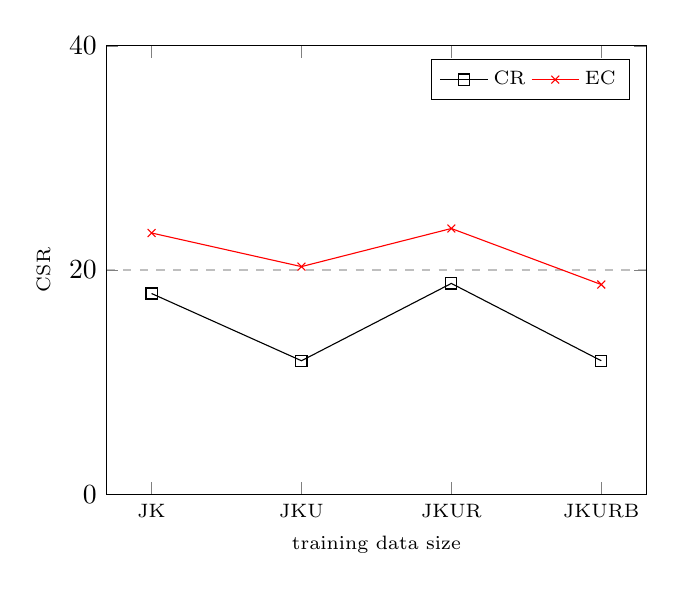
\begin{tikzpicture}
	\begin{axis}[
	title={},
	title style = {font=\scriptsize},
	xlabel={training data size},
	x label style={font=\scriptsize},
	x tick label style={font=\scriptsize},
	xtick=data,
	ylabel={CSR},
	y label style={font=\scriptsize},
	ymin=0, ymax=40,
	symbolic x coords={JK, JKU, JKUR, JKURB},
	ytick={0,20,40},
	legend pos=north east,
	legend style={legend columns=-1, font=\scriptsize},
	ymajorgrids=true,
	grid style=dashed,
	]
	
	\addplot[
	color=black,
	mark=square,
	]
	coordinates {
		(JK,17.9)(JKU,11.9)(JKUR,18.8)(JKURB,11.9)
	};
	
	\addplot[
	color=red,
	mark=x,
	]
	coordinates {
		(JK,23.3)(JKU,20.3)(JKUR,23.7)(JKURB,18.7)
	};
	\legend{CR, EC} 
	\end{axis}
	\end{tikzpicture}
	\caption{$maj/3$ performance v.s. training data size}
	\label{fig:4-datavsmaj3}
\end{figure}

\pgfplotsset{width=10cm,height=6cm,every node near coord/.append style={font=\scriptsize}}
\begin{figure}
	\centering
	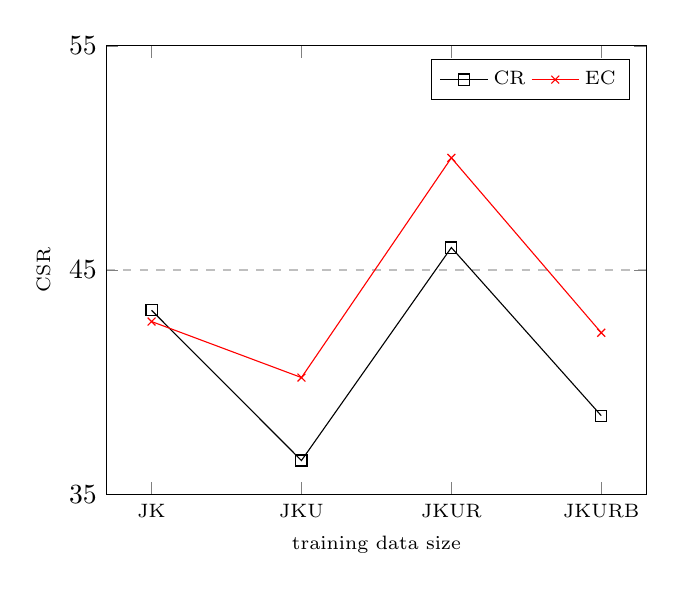
\begin{tikzpicture}
	\begin{axis}[
	title={},
	title style = {font=\scriptsize},
	xlabel={training data size},
	x label style={font=\scriptsize},
	x tick label style={font=\scriptsize},
	xtick=data,
	ylabel={CSR},
	y label style={font=\scriptsize},
	ymin=35, ymax=55,
	symbolic x coords={JK, JKU, JKUR, JKURB},
	ytick={35,45,55},
	legend pos=north east,
	legend style={legend columns=-1, font=\scriptsize},
	ymajorgrids=true,
	grid style=dashed,
	]
	
	\addplot[
	color=black,
	mark=square,
	]
	coordinates {
		(JK,43.2)(JKU,36.5)(JKUR,46.0)(JKURB,38.5)
	};
	
	\addplot[
	color=red,
	mark=x,
	]
	coordinates {
		(JK,42.7)(JKU,40.2)(JKUR,50.0)(JKURB,42.2)
	};
	\legend{CR, EC} 
	\end{axis}
	\end{tikzpicture}
	\caption{$maj/5$ performance v.s. training data size. Input: chromagram}
	\label{fig:4-datavsmaj5}
\end{figure}

A reasonable conjecture of why this might happen in EC is that the ground-truth labeling of chords, specifically in datasets U and B, are not consistent. Particularly, some inversion chords may be mislabeled as root positions or vice versa (for example, $maj/3$ labeled as $maj$ or vice versa) as they are sometimes easily confusable. There is a very good chance that this might happen and thus it introduces noise in the data, which could eventually blur the trained model's classification boundaries between these confusing chord pairs.
%While this conjecture might be true, a more solid justification demands a much deeper investigation into the labels of these datasets and the chord confusion matrices between these confusing pairs mentioned above. (say it when you have the data)


\subsection{System comparison}

\begin{table}[htb]
	\caption{Comparison between the proposed systems and Chordino - overall performance. Input: chromagram}
	\label{tab:4-cpcd}
	\centering
	\scriptsize
	\begin{tabular}{|c|c|c|c|c|c|c|c|c|c|c|c|c|c|}\hline
		System & \textit{MajMin} & \textit{MajMinBass} & \textit{Sevenths} & \textbf{\textit{SeventhsBass}} & Segmentation Quality\\ \hline
		JKURB & 70.6 & 68.7 & 56.3 & 54.7 & 78.0\\ \hline
		JKURB* & 70.1 & 68.2 & \textbf{57.6} & \textbf{56.0} & 76.8\\ \hline
		Chordino & \textbf{72.4} & \textbf{69.1} & 55.8 & 52.8 & \textbf{83.8}\\ \hline
	\end{tabular}
\end{table}

Finally, we would like to know how good is this LVACE approach compared with existing ones. Chordino\cite{cannam2013mirex} is used as a comparison baseline. It has a similar feature extraction module as the proposed systems and it supports a similar set of large vocabulary, which most of other ACE systems do not support. Chordino is an expert system (non-machine learning) that represents a very high standard \cite{deng2016chord} in terms of large vocabulary balanced performance.

Table~\ref{tab:4-cpcd} shows the comparison, in which there are two systems trained with the largest possible amount of data with different training schemes. In terms of overall performances, the proposed systems slightly outperform Chordino in terms of the strictest \textit{SeventhsBass} score, but slightly underperform Chordino in the more relaxed \textit{MajMin} and \textit{MajMinBass} scores.

% may need to change some wordings here, to sloppy
A large margin is found in segmentation quality, in which Chordino scores 5.3 and 7 points higher than the proposed systems. As noted previously, the segmentation quality is indeed a problem in this end-to-end approach. One could expect a boost of overall performance as well as balanced performance if the segmentation quality score could be raised to at least Chordino's level.

\begin{table}[htb]
	\caption{Comparison between the proposed systems and Chordino - long-tail and balanced performance. Input: chromagram}
	\label{tab:4-cpcd-2}
	\centering
	\scriptsize
	\begin{tabular}{|c|c|c|c|c|c|c|c|c|c|c|c|c|c|}\hline
		System & \textit{maj/5} & \textit{maj/3} & \textit{7/b7} & \textit{ACQA} \\ \hline
		JKURB & 11.9 & 38.5 & 4.9 & 14.7\\ \hline
		JKURB* & 18.7 & \textbf{42.2} & 24.0 & \textbf{18.4}\\ \hline
		Chordino & \textbf{ 27.6} & 29.8 & \textbf{24.4} & \textbf{20.9}\\ \hline
	\end{tabular}
\end{table}
Table~\ref{tab:4-cpcd-2} shows another set of comparisons in terms of long-tail and balanced performance. The CR system underperforms Chordino in all the presented categories except for $maj/3$.	The EC system outperforms Chordino in $maj/3$ and gets very close to Chordino in both $7/b7$ and $ACQA$. The latter results are very promising as they showcase that an end-to-end large vocabulary chord sequence classifier (JKURB*) could achieve a long-tail and balanced performance close to a manually engineered expert system (Chordino), with the help of the proposed even chance training scheme.

\section{Summary}\label{sec:4-concln}
This chapter proposes an end-to-end ``local feature extraction - global classification'' BLSTM-RNN based ACE system that supports SeventhsBass vocabulary. This system has a handcrafted feature extraction process, and can be compared with Chordino in a statistically fair way. To cater for large vocabulary recognition, an even chance training scheme is designed. Several variants of the system are trained and implemented. Evaluation results show some variants largely outperform Chordino in terms of large vocabulary scores, and they are almost as good as Chordino in terms of small vocabulary scores, despite having much worse segmentation qualities. It can be concluded that the proposed BLSTM-RNN architecture is better than the dedicated handcrafted GMM-HMM in terms of large vocabulary sequence modeling, but it suffers from bad sequence segmentation.

Through detail analysis of the results, a plausible issue of annotation inconsistency is identified. As suggested in Chapter~\ref{cp:background}, a workaround would be to always use annotations provided by one single source/annotator, or, to the other extreme, always use multiple annotators and apply majority vote or data fusion. But eventually, the ultimate evaluation tool may remain a fully subjective one, that let user experience to judge system performance.

Even chance training has been demonstrated very efficient in improving long-tail symbol recalls. It also boosts some VERY long-tail cases from zero score to non-zero. However, it sacrifices the performances of large population chords, and thus downgrades the overall performances in all but the versatility category.

To improve this system, the key thing to be done is to improve RNN's segmentation quality, since it determines an upper-bound of all other system performance, and the scores of all other metrics scale in proportion to segmentation quality. This can possibly be done through a dedicated segmentation training pass, a deeper RNN model, or combination of a segmentation-RNN with a annotation-RNN in a hierarchical way.




% ---------------------------------------------------------------------------
%: ----------------------- end of thesis sub-document ------------------------
% ---------------------------------------------------------------------------



% this file is called up by thesis.tex
% content in this file will be fed into the main document

\chapter{A Preliminary Approach to Automate Jazz Chord-Scale Estimation and Jazz Improvisation}\label{cp:jazz} % top level followed by section, subsection


% ----------------------- paths to graphics ------------------------


Previous chapters have explored ACE in \textit{SeventhsBass} vocabulary, which contains a limited amount of sevenths and inversions. This vocabulary is most used in music styles such as pop, rock, and folk songs. But chord types such as sevenths extensions, suspensions and alternations are not included in \textit{SeventhsBass}. This chapter, following the original large vocabulary spirit of Fujishima \cite{fujishima1999realtime} and Sheh \cite{sheh2003chord}, tries a preliminary ACE solution that covers a much larger vocabulary, and beyond that, puts together a ``chord-scale'' estimation system that could be deployed in an automated jazz improvisation platform.

% ----------------------- contents from here ------------------------
\section{Jazz Fundamentals} \label{sec:5-jazzfund}
This chapter focuses on a much larger vocabulary, including triads, sixths, sevenths and their extensions, suspensions, and alternations. In particular, it targets at jazz, which is a improvisation based style with complex harmonic structures \cite{hojnackijazz}:
\begin{quote}
One thing that distinguishes mainstream jazz harmony from other tonal styles is the tremendous amount of harmonic color that arises due to the pervasive use of tertian extensions of the basic chord types.
\end{quote}
Different from pop, rock and folk music, which usually have long chord progressions within the same key and only modulate at most a few times during a piece, jazz music often contains a lot of key modulations. A {\it modulation} is \cite{randel1999harvard}:
\begin{quote}
in tonal music, the process of changing from one key to another, or the result of such change.
\end{quote}
Musical key and chord progression are closely related to each other. Many MIR systems \cite{catteau2007probabilistic,noland2009influences,mauch2010simultaneous,papadopoulos2012modeling} have been attempted to extract both at the same time. But these works are basically all experimented under low modulation rate contexts. While under a jazz context, where modulation rate is much higher, these classical approaches may or may not apply. Hence besides ACE, this chapter will investigate on a different key tracking algorithm in order to also capture the modulations. It should be noted that in {\it modal jazz}, where a piece is constructed horizontally around the melody instead of vertically around the harmonics, the functional role of ``chord progression'' is weaken or eliminated, but there are still harmonic movements, regardless of keys or chords, to support the melody lines.

As jazz is an improvisation based music style, extracting chord progressions and key modulations could help determine/imply {\it chord-scale} candidates to improvise over a given harmonic segment. A {\it chord-scale} is \cite{hojnackijazz}:
\begin{quote}
a linear rendering of a complex chord - an extended chord structure, with tensions and non-chord tones arrayed within an octave.
\end{quote}
Each chord-scale is constructed by a root and a scale, where the root is similar to the root of a chord. As for the scale, there are seven commonly used scales in jazz that are derived from the \textit{major} scale, each of those is called a {\it mode} or {\it modal scale}. They are:
\begin{enumerate}
\item Ionian: $WWHWWWH$
\item Dorian: $WHWWWHW$
\item Phrygian: $HWWWHWW$
\item Lydian: $WWWHWWH$
\item Mixolydian: $WWHWWHW$
\item Aeolian: $WHWWHWW$
\item Locrian: $HWWHWWW$
\end{enumerate}
The ``W'' and ``H'' indicate the seven sequential whole/half step intervals within the scale (note that $W$ = $2*H$). These modes, from 1 to 7, can be memorized as left-circular shifting the \textit{major} scale ($WWHWWWH$) one note at a time. Similarly, modes can also be built based on {\it harmonic minor scale} ($WHWWHW^+H$, where $+$ means an additional half step) or {\it melodic minor scale} ($WHWWWWH$). Alternatively, there could be other scales out of this construction methodology, such as the {\it whole-half diminished scale} ($WHWHWHWH$), {\it half-whole diminished scale} ($HWHWHWHW$), {\it whole-tone scale} ($WWWWWW$) or {\it chromatic scale} ($HHHHHHHHHHHH$).

Normally, a chord-scale is chosen based on the current musical key context, which is determined by the underlying {\it harmonic functional group} \cite{hojnackijazz,levine2011jazztheory}. Table~\ref{tab:5-chordscale} show some choices suggested by a jazz guitar tutorial book \cite{jazzguitarbook}. For a specific chord type, there could be multiple choices of scales, but the best picks will be determined by the musical key context, where the scale of choice cannot strongly indicate otherwise.
\begin{table}
\centering
\footnotesize
\begin{tabular}{|c|c|} \hline
Chord & Scale \\ \hline
\textit{7} & Mixolydian, Phrygian-Dominant, Whole-tone \\ \hline
\textit{maj7} & Lydian, Lydian-Dominant, Ionian, Ionian\#5 \\ \hline
\textit{min7} & Dorian, Phrygian, Aeolian \\ \hline
\textit{min7b5} & Locrian, Locrian\#2 \\ \hline
\textit{7b9} & Phrygian-Dominant \\ \hline
\textit{maj7\#11} & Lydian \\ \hline
\textit{maj7\#5} & Ionian\#5 \\ \hline
\textit{dim7} & Whole-half Diminished \\ \hline
\end{tabular}
\caption{Chord-scale choices examples}
\label{tab:5-chordscale}
\end{table}

Chord-scale system is a good way to analyze jazz harmony and melody. But in real improvisation, jazz musicians seldom think of the chord-scale system. Instead, they memorize all these by heart and improvise using the variations of melody passages and patterns they learn through extensive exercises \cite{jazzguitarimpro}. To be precise, instead of generating notes from the scales, they generate phrases that belong to the chord-scale. Infinity number of note sequences can be created out of the chord-scale, but those phrases, within all these sequences, are among the most acceptable ones to human musical aesthetics. In addition to creating phrases within a single harmonic region, they also pay much attention to the coherence along all different phrases so as to make as much musical sense as possible.

\section{Automatic Jazz Chord Estimation} \label{sec:5-jazzace}
To do ACE for jazz, the system framework in Chapter~\ref{cp:ghmm} is used. Assuming the segmentation pass can achieve a high output quality, the remaining task is to classify chords independently in each segment. Figure~\ref{fig:5-jazzsys} is a succinct version of the system framework, where the segment tiling process is absorbed in the chord classifier module.
\begin{figure}[htb]
    \centering
        \includegraphics[width=0.8\columnwidth]{5/figures/sys.pdf}
    \caption{The Jazz ACE system. It is equivalent to the system in Figure~\ref{fig:3-sysover}}
    \label{fig:5-jazzsys}
\end{figure}

Table~\ref{tab:5-aceconfig} shows all ACE configurations considered in the experiment. They are chosen based on the results in Chapter~\ref{cp:ghmm}.
\begin{table}
\centering
\footnotesize
\begin{tabular}{|c|c|c|} \hline
Dimension & Configuration \\ \hline
Deep learning system & FCNN, DBN, BLSTM-RNN\\ \hline
Hidden layers & (800,800)\\ \hline
Segment tiling & 6\\ \hline
Feature level & notegram(-ns), chromagram (-ch) \\ \hline
\end{tabular}
\caption{ACE configurations}
\label{tab:5-aceconfig}
\end{table}

\subsection{Experimental Setup}
In this study, 99 pieces of jazz chord comping + soloing dataset extracted from a jazz guitar book \cite{jazzguitarbook} (JazzGuitar99) are used as training/validation dataset, and 7 pieces from Gary Burton's on-line course \cite{garyburtoncourse} (GaryBurton7) are used as test dataset. JazzGuitar99's annotations are taken directly from the book, and GaryBurton7's annotations are taken from the leadsheets provided along with the course. The vocabulary has 36 types \footnote{They are: $maj$, $min$, $min6$, $6$, $maj7$, $maj7\#5$, $maj7\#11$, $maj7b5$, $min7$, $minmaj7$, $min7b5$, $min7\#5$, $7$, $7b5$, $7b9$, $7\#9$, $7\#5\#9$, $7\#5b9$, $7b5b9$, $7\#5$, $7sus4$, $aug7$, $dim7$, $ maj9$, $min9$, $9$, $9\#11$, $min11$, $min11b5$, $11$, $min13$, $maj13$, $13$, $13b9$, $69$ and $N.C.$}.

%In the second study, the training/validation dataset is extracted from the CDs of a jazz guitar improvisation tutorial \cite{jazzguitarimpro} (JazzImpro96) and a practical jazz guide \cite{pracjazz} (PracJazz76). Totally they contain 172 tracks. All annotations are taken from the leadsheets in the books. The datasets of the previous study is used for testing. The vocabulary has 60 types\footnote{$maj7$, $min7$, $7$, $maj7\#11$, $min9$, $9sus4$, $7sus4$, $maj$, $7b9$, $9$, $13$, $9\#11$, $7\#9$, $min7b5$, $min$, $minmaj7$, $min6$, $7b13$, $7(9, \#11, 13)$, $7\#5$, $6$, $maj9$, $7(b9, \#9, b13)$, $7(b9, b13)$, $7(\#9, b13)$, $7(\#9, b9)$, $7\#11$, $9(b9, b13)$, $69$, $13b9$, $9b13$, $7(9, \#11)$, $7(13)$, $9(13)$, $7(alt)$, $dim7$, $min7(11)$, $7(b9, 13)$, $7(\#11, 13)$, $min7b9$, $7(9, 13)$, $7(9)$, $min7b5(11)$, $7\#5(\#9)$, $min7(11, 13)$, $9(6)$, $aug7$, $7b5$, $maj13$, $min11$, $7\#5\#9$, $11$, $min13$, $7\#5b9$, $maj7\#5$, $min11b5$, $maj7b5$, $min7\#5$, $7b5b9$ and $N$}.

All training data are to be used at either notegram (-ns) or chromagram (-ch) level, which does not contain phase information. Assuming 12-tone equal temperament, they can be augmented by pitch shifting with zero padding (for -ns), or circular pitch shifting (for -ch) to all 12 keys. Adjusting the chord labels accordingly, this results in 12 times of training data.

Note that inversions are not considered in this preliminary jazz ACE study because: 1. there are very few inversion notations in the currently used datasets; 2. it results in a huge number of classes.

\subsection{Results and Discussion}
Following the MIREX ACE convention, system performance on jazz chord vocabulary is evaluated based on \textit{WCSR}. The \textit{WCSR} computing procedure in its fairest/strictest sense should regard each chord as it is without applying any sort of mapping scheme, as happens to \textit{SeventhsBass}. In the following each system is evaluated in this way. The baseline is an augmented Chordino with jazz vocabulary extension (Jazz-Chordino). The augmentation is done within its GMM-HMM engine by applying the jazz chord dictionary to the Gaussian model, whose setting is given in Table \ref{tab:5-jcgau}.
\begin{table}[h]
\centering
\footnotesize
\begin{tabular}{|c|c|c|} \hline
      & $\mu$ & $\sigma^2$ \\ \hline
Bass - Chord Bass & 1 & 0.1 \\ \hline
Treble - Chord Note & 1 & 0.2  \\ \hline
Neither bass nor treble & 0 & 0.2 \\ \hline
N.C. (for all notes)  & 1 & 0.2  \\ \hline
\end{tabular}
\caption{Gaussian model of Jazz-Chordino}
\label{tab:5-jcgau}
\end{table}

All systems are tested using GaryBurton7 dataset \footnote{Composition of chords in GaryBurton7: \textit{maj}:0.09; \textit{min7}:0.13; \textit{7}:0.22; \textit{min7b5}:0.12; \textit{7b9}:0.06; \textit{min}:0.1; \textit{maj}:0.14; \textit{others}:0.14.}. Results are shown in Table \ref{tab:5-jazz-wcsr}. Jazz-BLSTM system performs the best, and outperforms Jazz-Chordino by about 10 points. The ranking is very similar to \textit{SeventhsBass}', but the results are in a sense more convincing, since the test set is not dominated by chords like \textit{major} and \textit{minor}. In fact the chord composition in GaryBurton7 is relatively balanced, though rare chords are still rare. These results demonstrate the advantage of the proposed system framework for very large chord vocabulary.

Meanwhile, notice that the \textit{SQ} (segmentation quality) of these systems are all relatively high, and these are achieved in pure jazz test audio. All systems use Jazz-Chordino's GMM-HMM as segmentation engine. The differences between \textit{SQ} scores are caused by different merging of consecutive chord boundaries in different systems. Obviously the success of Jazz-BLSTM owes to the success of the GMM-HMM segmentation at the beginning; then based on the segmentation it performs classifications without taking care of chord progression context.
%This task is comfortable to deal with by a fixed-length input deep learning model. The advantage may not be obvious under a small chord vocabulary, but is obvious under a large chord vocabulary.

\begin{table}[t]
\centering
\footnotesize
\begin{tabular}{|c|c|c|} \hline
systems & \textit{WCSR} & \textit{SQ}\\ \hline
Jazz-Chordino & 57.99 & 81.68\\ \hline
Jazz-FCNN-ns & 61.81& 76.18\\ \hline
Jazz-DBN-ns & 62.33& 80.73\\ \hline
\textbf{Jazz-BLSTM-ns} & \textbf{66.41} & 80.78\\ \hline
\textbf{Jazz-FCNN-ch} & \textbf{65.65} & 81.94\\ \hline
Jazz-DBN-ch & 4.56& 20.42\\ \hline
Jazz-BLSTM-ch & 63.72 & 82.22\\ \hline
\end{tabular}
\caption{Jazz ACE performances}
\label{tab:5-jazz-wcsr}
\end{table}

\subsection{Extension - Jazz Scale Estimation}
The above preliminary jazz ACE system can be extended to jazz scale estimation, thereby achieving a unified chord-scale estimation approach. As reviewed in Section~\ref{sec:5-jazzfund}, the scales are chosen based on the harmonic functional group, which establishes a temporary tonal center, or a key. Consequently, a natural approach to do jazz scale estimation is by imitating local key estimation.
\begin{figure}[htb]
    \centering
        \includegraphics[width=0.6\columnwidth]{5/figures/localscale.pdf}
    \caption{Template-based local scale tracking. A scale is estimated within a context window of chords.}
    \label{fig:5-localscale}
\end{figure}
Figure~\ref{fig:5-localscale} shows the extended ACE system for local scale estimation, where ``chordo'' means the conditional probabilities of each chord given the chroma as input. Different from the chord-key estimation systems proposed by Mauch \cite{mauch2010simultaneous} and Catteau \cite{catteau2007probabilistic}, the scale is not estimated by a generative model, but a discriminative template-based model similar to Rocher et al.'s chord-key estimation approach \cite{rocher2010concurrent}. Instead of using a well-known key profile \cite{temperley2004cognition}, binary ``scale templates''($ST$) are used to compute a local scale posterior probability surface from the ``chord templates''($CT$), similar to the key estimation method in \cite{hu2015safedj}. Since each local scale cannot be determined by just one chord, a context window is introduced to collect a 3 chords neighborhood:
\begin{equation}
\text{fit} = \sum_i^{12} ST_i \times {\sum_{j=1}^3 CT_{ij} \over 3},
\end{equation}

For each chord, the system will decide a list of scale candidates from a look-up-table, then pick the one with the best fit score:
\begin{equation}
scale = \max_k (\text{fit}_k).
\end{equation}
The template-based local scale estimation is implemented during the ISMIR 2016 Hackathon \footnote{http://labrosa.ee.columbia.edu/hamr\_ismir2016/}. Figure~\ref{fig:5-chordscale} shows an example of the output of this estimation process with ``Olhos de Gato'', where the labels in red indicate the estimated scales.
\begin{figure}[h]
    \centering
        \includegraphics[trim={0 4cm 0 2cm},clip,width=0.8\columnwidth]{5/figures/chordscale-demo.pdf}
    \caption{Chord-scale tracking demo output from a leadsheet}
    \label{fig:5-chordscale}
\end{figure}

However, since this is a relatively new direction in MIR, there is not any well-established labeled dataset available for performance testing. Therefore this module has not been formally evaluated under any objective measure yet.

The research of jazz chord-scale estimation has its straightforward application in new musical expression interfaces. In the remaining parts of this chapter, two mobile jazz improvisation platforms will be introduced in Section~\ref{sec:5-wijam} and ~\ref{sec:5-akb}. Finally, Section~\ref{sec:5-puttogether} will seek to put the chord-scale estimation system in a fully automatic jazz improvisation context.

\section{Jazz Improvisation Platform - WIJAM} \label{sec:5-wijam}
WIJAM is an impromptu iOS mobile application for a group of musical novices to jam along with a music master. The master provides backings, directs the musical flow and gives feedbacks to the players. The players improvise along with the master's guidance.

WIJAM, according to Weinberg\cite{weinberg2005interconnected}, is a ``small-scale local system", which can be characterized as ``collaborative musical network ... that support three to ten players in close proximity, which allows for detailed and subtle interpersonal interactions". Under the ``theoretical framework of musical interconnectivity''\cite{weinberg2005interconnected}, WIJAM can be considered structure-centered and process-centered, where ``structure'' is manifested in the absolute musical arrangement control of WIJAM master, and ``process'' is done when WIJAM players express intuitively their musical feelings within the bounds as defined by the WIJAM master.

In terms of organization and architecture, WIJAM is a ``synchronous centralized network'' with a ``flower topology'', where music is being generated in real-time with a central hub, and the degrees of freedom in terms of the nodes' expression are limited to a level such that the musical outcomes are at least musically harmonious.

\subsection{Design Concepts}
WIJAM's design follows Blaine's guidance \cite{Blaine2003}:
\begin{quote}
The underlying premise of most collaborative interface design is that with various design constraints, playing music can be made accessible to non-musicians ... at the expense of limiting the musical range and possible gestures associated with sound in a collective space.
\end{quote}
But as pointed out in the same paper, such a guideline has its drawback:
\begin{quote}
... many of the simple-to-use computer interfaces proposed for musical control seem, after even a brief period of use, to have a toy-like
character and do not invite continued musical evolution.
\end{quote}
Although the paper goes on to argue that this is only true for expert musicians, but ``balancing this trade-off is a key concern for designers", as pointed out in \cite{blaine2003collaborative}. This point is echoed in many other papers\cite{xambo2011multi}, emphasizing that ``provide novices with essential goals and experts with additional goals". Trying to meet this balance, WIJAM equips the players with an easy to learn and easy to play keyboard, while at the same time providing ``a knowledgeable person to stand by and assist the players" \cite{Blaine2003}--the master. The players performance bound is imposed upon by the master, which should give a large enough space for the players to show off their virtuosity.

\subsection{System Overview}
Figure~\ref{fig:5-BigPicture} shows the big picture of WIJAM. There are two types of active entities: the master, who initiates and orchestrates the jamming, and the players who participate in the jamming. There is a passive entity: a loudspeaker system, which is connected to the master.

\begin{figure}[htbp]
    \centering
        \includegraphics[width=0.6\columnwidth]{5/figures/BigPicture.png}
    \caption{The big picture of WIJAM. The music collaboration is achieved under the ``master-players" paradigm.}
    \label{fig:5-BigPicture}
\end{figure}

Figure~\ref{fig:5-FlowChart} is the flowchart of the WIJAM session process. At the beginning, the master hosts a \textit{MIDINetworkSession} as a jam session service to be discovered and connected to. Then the players join the session. After that the master sends an ``assignment" package to each player. The package contains an instrument ID, and a chord-scale. The master signals the start of the jam by switching on the backing music. When the players start to jam, they send MIDI performance contents to the master via \textit{coreMIDI}. The master monitors all the performance, renders the notes in the chosen instrument sounds and mixes them with the backing into one output stream. While jamming, the master orchestrates everything to fit to the backing music by instantly changing the assignment or providing performance cue feedbacks to the players such as ``good", ``solo", ``fast", ``calm", etc. When they finished jamming a song, the master gives an overall score as well as an individual score to the players.
\begin{figure}[htbp]
    \centering
        \includegraphics[width=0.6\columnwidth]{5/figures/Flowchart.png}
    \caption{The flowchart of WIJAM.}
    \label{fig:5-FlowChart}
\end{figure}

\subsection{Master Machine}

\begin{figure}[htbp]
    \centering
        \includegraphics[width=0.6\columnwidth]{5/figures/MasterVC.jpg}
    \caption{WIJAM's Master Interface}
    \label{fig:5-MasterVC}
\end{figure}

The internal structure and layering of the master machine \footnote{https://github.com/tangkk/MasterMachine.git} is shown in the middle part
of Figure~\ref{fig:5-Layering}. The core modules are detailed below:
\begin{figure*}[htbp]
    \centering
        \includegraphics[width=0.8\textwidth]{5/figures/Layering.png}
    \caption{The internal layering and structure of WIJAM. The data flows from the master machine (middle) to the player machine (right) through the bidirectional communication channel, and vice versa.}
    \label{fig:5-Layering}
\end{figure*}

\Hsection{Master Interface}
The master interface is shown in Figure~\ref{fig:5-MasterVC}. In the top left corner there is a backing selector which allows the ``master" to initiate the backing music. Moving downwards there is a chord-scale panels. They are particularly important for orchestrating the musical flow. At the bottom there are six consoles, from A to F, each for an individual player. They provide performance feedback to the players as well as music output level balancing.

\Hsection{Arranger}
This allows the master to manipulate chords, scales, instruments, and feedbacks. These messages are sent via \textit{MIDI sysEx} messages.

\Hsection{Virtual Instruments}
It stores a library of digital musical instruments in the form of samplers. The audio samples are managed using \textit{AUPreset} and \textit{AUSampler} technologies\cite{AUSampler}. The \textit{AUPreset} files are used to map audio samples directly to MIDI numbers and velocity ranges.

\Hsection{Jam Session Host}
It hosts a service which can be discovered and connected to by the player machines. \textit{MIDINetworkSession} is used to enable a \textit{Bonjour} service. It is to be discovered by the player machines' Bonjour service browsers, and to be connected to by the player machines' \textit{MIDINetworkSessions}.

\subsection{Player Machine}
The player machine's layering is described on the right hand side of Figure~\ref{fig:5-Layering} and its interface on Figure~\ref{fig:5-PlayerMachineVC} with the jam console on the left and the keyboard on the right. \footnote{https://github.com/tangkk/PlayerMachine.git} The jam console is designed to discover and connect to the master machine, and the keyboard is for musical expression. The following items summarize the working mechanism of the keyboard:
\begin{figure}[htbp]
\begin{center}$
\begin{array}{cc}
\includegraphics[width=1.2in]{5/figures/PlayerMachineVC.png} &
\includegraphics[width=1.2in]{5/figures/Simple.png} \\
\end{array}$
\end{center}
\caption{WIJAM's Player Interface}
\label{fig:5-PlayerMachineVC}
\end{figure}
\begin{itemize}
\item
The y position determines the pitch, where higher position yields higher pitch.
\item
At any time the keyboard is filled with the chord-scale assigned by the master machine.
\item
The x position determines the note velocity. A larger x position value gives higher velocity.
\item
When sketching, a note is generated when the it starts or when the curve comes to a stationary point.
\end{itemize}
This keyboard is easy to use for novice players, by abstracting away most complicated musical context. It allows the players to do a high-level melody improvisation.

\subsection{Demos}
There are two basic demos \footnote{\url{http://www.youtube.com/watch?v=Y0PnKBrgzgw}} and one advanced demo \footnote{\url{http://www.youtube.com/watch?v=16dWj5G9UKw}} for WIJAM. The basic demo shows how WIJAM works, and provides tips for using the master machine and the player machine. The audio track is an unmodified recording of the original playback. Before the jam starts, the players are told to follow their ``musical feelings" based on the backing. As can be heard in the video, the music outcome is quite pleasing, even at the critical ``key modulation" points: 2:30 and 2:43. Note that as the jam goes on, because the players have little idea about what the exact notes they are playing, the ``avoid note", the most dissonant note within the chord-scale, may be played on downbeat. This may happen, but with a very small chance.

The ``trombone" player and the two ``guitar" players are with zero training in musical instruments. The ``piano" player has some limited
experience with piano before. Even so, the piano player is able to inject a very beautiful solo during the jam. The ``piano" player apparently plays the best music in this jam session. This somewhat justifies the ``balance" problem in the ``Introduction" section of this Section, in that WIJAM actually allows advanced players to show off their virtuosity while also enabling an acceptable level of performance for the novice players.

The advanced demo is a bonus track featuring the designer of WIJAM playing and overdubbing a whole jam session. It shows some advanced features of the PlayerMachine. The audio track is an overdubbing of each instrument track plus the backing track.

\section{Jazz Improvisation Platform - ArmKeyBoard} \label{sec:5-akb}
The piano keyboard, although is versatile and popular, has a lot of drawbacks. The same type of chord or scale in different keys are laid out differently, which adds to the learning difficulty. Additionally, the keyboard has a linear layout of the black and white keys, which works well with music expressions that exhibit certain linearity , but is less effective for modernistic non-linear styles such as that of serialistic and stochastic music \cite{Mitsuko:Schoenberg}.

Trying to solve the above problems, a new type of keyboard is designed. Based on the NIME design principles \cite{cook2001principles}--specifically the ``Make a piece, not an instrument or controller" and ``Instant music, subtlety later"--the keyboard leverages a chord-octave-scale sequence grid to pack 88 keys into a 15--17 keys-sized screen, and features an almost zero learning curve for the production of beautiful and sophisticated melodies. It offers both linear and non-linear layouts. The non-linear layout is mapped to a user chosen image by an algorithm based on contour separation and tonal hierarchy. This is called ``ArmKeyBoard", where ``ArmKey" means suitable, comfortable, and in-tune, in the author's spoken dialect.

\subsection{Two Types of Keyboard Layout}
In the remaining discussion, ``keyboard" refers to an instrument implementing a series of key-note pairs and deterministically
generates a note when a key is pressed. ``Layout" refers to the spatial arrangement of those key-note pairs.

Linear layout is characteristic of a piano. From left to right, each key is mapped to a unique note value. Every next key is mapped to
a note value exactly 1 (in MIDI terms) higher than the previous one. This has a significant impact on music making, since people naturally feel more comfortable with playing on adjacent keys than non-adjacent keys, leading to smaller intervals appearing more often than larger ones, as can be seen in music literature such as \textit{the Real Book} \cite{therealbook6th}.

Non-linear layout can have many more possibilities, such as a random note being paired with a random key or one note being paired with
several keys. Note that in the current discussion, several notes being paired with one key is not valid by the definition of keyboard. Non-linearity may further allow using any key setting other than the traditional setting. For example an image can be divided into several sections, each serving as a key of the keyboard. The idea of non-linear keyboard is not new. There are existing applications such as \cite{kontakts} or papers such as \cite{kruge2011madpad} talking about similar ideas, most of which are built around the idea of sampling. In Armkeyboard, however, the audio content generated by a key is a note.

\subsection{Chord, Scale and Octave}
ArmKeyBoard treats the small screen as a cache, caching the currently playing chord-scale in the current octave range, while other
octaves and chord-scales are waiting to be loaded when needed. In the current design, 15--17 notes---two octaves of a scale, are cached

Changing chord-scale or octave on a piano in real time is easy for a pianist, but could be a nightmare for non-pianists. Therefore, ArmKeyBoard needs a special mechanism to load other chord-scales and octaves into the foreground, so that the player can easily switch music expression ranges in real time. To this end, a chord-octave-scale sequence grid as shown in Figure~\ref{fig:5-cosgrid} is designed.
\begin{figure}[htbp]
\begin{center}$
\begin{array}{cc}
    \includegraphics[width=1.2in]{5/figures/ChordOctaveScaleGrid.PNG} &
    \includegraphics[width=1.2in]{5/figures/ChordScalePreset.PNG}\\
\end{array}$
\end{center}
\caption{On the left is the chord-octave-scale grid, where each square can be set as one chord-octave-scale
combination (such as C-4-Lydian), and consecutive squares form a sequence which can be saved as preset; The sequence is read from left to right, and when it reaches the rightmost, back to the leftmost square on the next line; On the right is the chord-octave-scale preset browser looking at the already saved chord-octave-scale sequence presets.}
\label{fig:5-cosgrid}
\end{figure}

\begin{figure}[htbp]
\begin{center}$
\begin{array}{cc}
\includegraphics[width=1.2in]{5/figures/Gravity0.jpg} &
\includegraphics[width=1.2in]{5/figures/GravityX.jpg} \\
\end{array}$
\end{center}
\caption{Gravity X gesture, which is used for switching to the next or previous page of notes determined by the chord-octave-scale combination at the next or previous square within the sequence.}
\label{fig:5-GravityXGesture}
\end{figure}

Users can switch between different chord-octave-scales using a gravity X gesture (Figure~\ref{fig:5-GravityXGesture}). Meanwhile, users can also flip octaves within the same chord-scale using swipe gestures. To summarize, in Figure~\ref{figChordOctaveScaleControl}, the screen is a cache of the active note space, while the spaces around the active space can be loaded in real-time via gravity X or swipe gestures.

\begin{figure}[htbp]
\centering
\includegraphics[width = 3.2in]{5/figures/ChordOctaveScaleControl.png}
\caption{Chord-octave-scale control. The horizontal arrows indicate changing page of notes according to chord-octave-scale sequence, while the vertical arrows indicate changing page of notes to a higher or lower octave only.}
\label{figChordOctaveScaleControl}
\end{figure}

\subsection{Expression Parameters}
Because the proposed design is based on the piano keyboard, the most dominant expression parameter, velocity, should be implemented. In the
linear layout, since key-note mapping is 1-to-1 and the position of each key is equally distributed along the y-axis, velocity can be easily controlled by position X. While in the non-linear layout, position X cannot be used because keys can be in any shape and anywhere; thus Gravity Y is used to control the velocity (Figure~\ref{fig:5-GravityYZGesture}). Note that sustain is not considered in the current design, since if a hand gesture were to convey what is originally conveyed by foot, it might make learning difficult for the ordinary users. A gravity Z gesture is to restart the keyboard again (Figure~\ref{fig:5-GravityYZGesture}).
\begin{figure}[htbp]
\begin{center}$
\begin{array}{cc}
\includegraphics[width=1.2in]{5/figures/GravityY.jpg} &
\includegraphics[width=1.2in]{5/figures/GravityZ.jpg} \\
\end{array}$
\end{center}
\caption{Gravity Y gesture (on the left), which is used for controlling note velocity, leading to a smaller velocity with a larger angle to the horizontal plane; Gravity Z gesture (on the right), which is used for quitting the current keyboard to reset everything again}
\label{fig:5-GravityYZGesture}
\end{figure}

\subsection{Linear Layout and Mapping}
ArmKeyBoard has both linear and non-linear keyboard layout, called ``AKB1" and ``AKB2" respectively. The discussion is based on the iOS platform.

``AKB1" (Figure~\ref{fig:5-AKB12}) contains 15--17 notes within the active chord-octave-scale and they are mapped linearly to 15--17
bars equally divided along the y-axis. The velocity is controlled by the X position.

\subsection{Non-linear Layout and Mapping}
``AKB2" is a user selected image (Figure~\ref{fig:5-AKB12}). The image is algorithmically divided into contours and they are algorithmically mapped to the 15--17 notes within the currently active chord-octave-scale. The algorithms are described below.
\begin{figure}[htbp]
\begin{center}$
\begin{array}{cc}
\includegraphics[width=1.2in]{5/figures/AKB1.PNG} &
\includegraphics[width=1.2in]{5/figures/AKB2.PNG} \\
\end{array}$
\end{center}
\caption{AKB1 (on the left) is a linear keyboard with a higher pitch at smaller y position value, and larger note velocity at larger x position value, each page contains 15--17 notes; AKB2 (on the right) is a non-linear keyboard mapping the page of 15--17 notes to the detected contours within the user selected image, where the mapping procedure is based on the correlation between the importance of contours (or regions) and the tonal hierarchy of notes.}
\label{fig:5-AKB12}
\end{figure}

\Hsection{Contour Separation}
The contour separation is processed using opencv \cite{opencv}. The image is first transformed to opencv \textit{Mat} which is then passed to a contour separation function. The function then: Step 1, turns the \textit{Mat} into gray scale and slightly performs a blur operation on it; Step 2, passes the output of step 1 (a gray scale \textit{Mat}) to an edge detection function (the output is a binary \textit{Mat} with the edge pixels set as step 1); Step 3, passes the output of step 2 to a \textit{findContour} function, which finds contours, stores them in an array and calculates the contour hierarchy (a tree structure describing the inclusion relationship of contours); Step 4, calculates the area of each contour, discards those below a certain size and deletes their nodes in the hierarchy; Step 5, creates an outer contour which is the whole screen subtracted by all the contours output by step 4. The output of all the above steps is an array of valid contours (each contour is itself an array of its vertices), and a hierarchy structure describing the inclusion relationship of these contours.

\Hsection{Contour Ranking}
Next step is to decide which note to map to which contour. The minimal musical concern is, when the keyboard is being played, the notes being generated should at least imply the currently active chord-scale most of the time. Note that it is not necessary that it should ``always" behave this way, but ``most of the time". For example, in \textit{G-Ionian}, the keyboard is supposed to generate notes that form a tonal gravity at G and imply G major chord most of the time, but sometimes it may also sound like \textit{C-Lydian} (tonic at C).

More assumptions are needed to connect this musical concern to contours. Assume that most user tends to tap on: 1, a contour with a larger area; 2, a contour closer to the center of the screen; 3, a contour that contains more sub-contours. Based on how often most users will tap on a contour, its importance can be determined. Thus in the implementation, contours are ranked based on the weighted sum of
the above three indices. This corresponds to how important a note is in implying a certain chord-scale, which will be discussed below.

\Hsection{Tonal Hierarchy}
Similar to ranking contours, if the notes within a chord-scale is also ranked, then what is left is to map the two rankings. According to \cite{jarvinen1995tonal}, there is a certain tonal hierarchy within a chord-scale being played in bebop style jazz music, and this finding actually corresponds to the avoid note issue \cite{nettles1987harmony}. The tonal hierarchy theory says during the performance of a certain chord-scale, some notes are more often heard than others.

If the notes are to be divided into a hierarchy according to how often they appear, the first class contains chord tones (or chord notes), the second class contains those a whole step above the chord notes and finally those half step above, with exceptions. The avoid note issue expresses basically the same idea, but with ``more often heard" replaced by ``more often played".

Table~\ref{tab:5-tonalhierarchy} is a result of the tonal hierarchy theory, which lists all the hierarchies \cite{nettles1987harmony} of some of the most frequently used chord-scales \cite{burtonJazzImpro}. The scale degree notation is
used instead of note names. Note that symmetrical diminished scale and it has no hierarchies in this taxonomy. To deal with hierarchy across octaves, a heuristic rule is that the same pitch-class belongs to the same hierarchy level and a lower octave pitch has a higher priority than a higher octave pitch.

\begin{table}
\centering
\caption{Tonal Hierarchies in ArmKeyBoard. L1 is the first level of notes which are to be mapped to regions with highest importance, and L2 to be mapped to regions with second highest scores, then L3 to be mapped to the least important regions.}
\begin{tabular}{|c|c|c|c|} \hline
Scale & L1 & L2 & L3\\ \hline
Lydian & 1, 5, 3, 7& 2, \#4, 6 & \\ \hline
Ionian & 1, 5, 3, 7& 2, 6 & 4\\ \hline
Mixolydian & 1, 5, 3, b7 & 2, 6 & 4\\ \hline
Dorian & 1, 5, b3, b7& 2, 4 & 6\\ \hline
Aeolian & 1, 5, b3, b7& 2, 4 & b6\\ \hline
Phrygian & 1, 5, b3, b7& 4 & b2, b6\\ \hline
Locrian & 1, b5, b3, b7& 4, b6 & b2\\ \hline
Lydian b7 & 1, 5, 3, b7& 2, \#4, 6 &\\ \hline
Altered & 1, 3, b7& \#4, b6, b2, \#2 & 5\\ \hline
Whole-half Diminished & none & none &\\ \hline
Melodic Minor & 1, 5, b3, 7& 2, 4, 6 &\\ \hline
\end{tabular}
\label{tab:5-tonalhierarchy}
\end{table}

\Hsection{The Final Mapping}
The final mapping is not so obvious as it may seem. Although there are already a ranking of contours and a ranking of 15--17 notes within a chord-scale, they are by no means simply 1-to-1 mappings, because in reality it is not clear how many contours there are and how large each of them is until the user selects an image. In view of this complication, a heuristic based algorithm is devised to do this final mapping:
\begin{algorithm}
\caption{Contour-Note mapping}
\begin{algorithmic}
\STATE
1. Divide the screen size by the number of notes, and name the result $RPN$.
\STATE
2. Look at the $ ratio = Area(contour) / RPN $ of the top item of the sorted contour list (regarded as a stack). \newline If $ratio>=1$, do step	3; otherwise do step 4. Repeat until no contour left in the stack.
\STATE
3. Map notes to contour: pop the contour, pop the top $ ceil(ratio)$ notes and pair them up. Go back to step 2.
\STATE
4. Map contours to note: pop the contour, pair it up with the first	note. Add $ratio$ to $accum$. If $accum>=1$, clear $accum$ and pop the note. Go back to step 2.
\end{algorithmic}
\end{algorithm}
With this, the most important notes are mapped to the most important contours, and contour with larger areas will contain more notes. But since multiple notes cannot be mapped to a single key, they need to be decoupled  within a contour that has more than one note. Instead of further separating a shape-unpredictable contour into several sub-contours, it should be noted that the real ``key" in question is composed of pixels, and thus a heuristic method is used to decouple the notes is to distribute their keys across the contour according to a formula related to pixels and their RGB value:
\begin{equation}
\mathit{noteIdx = ((X + Y) \% 10 + (R + G + B)) \% (15\ or\ 17)}
\end{equation}
Where 15 or 17 is the number of notes. This whole scheme tries to make position affect less
and RGB affect more, while making sure all the notes are included regardless of the image.

\subsection{Demos}
There is a demo of Armkeyboard \footnote{\url{https://www.youtube.com/watch?v=ZhTleEXKeu4}}. The first part shows Armkeyboard's performance on a jazz backing track, and the second part shows a few solo performances. Besides the demo, the author has also applied Armkeyboard in Gary Burton's on-line jazz improvisation course to complete the peer reviewed assignments. In all 6 assignments, it gets an average of 3 points out of the maximum 5 points.


\section{Putting It Together}\label{sec:5-puttogether}
The modules in Section~\ref{sec:5-jazzace} to ~\ref{sec:5-akb} can be put together and form a semi-automatic or fully automatic jazz improvisation machine. The differences among these approaches are the way they deal with generation of note sequence within a chord-scale context.

\subsection{Chord-scale informed user improvisation}
The simplest form would be to only provide the platform with timed chord-scale sequence information, and let players input note sequence. First the jazz backing track is analyzed into segmented chord-scale sequence, then it is programmed into the improvisation platform. These information can automatically guide users with little musical knowledge to improvise jazz with at least the proper choice of chord-scale.

\subsection{Markov model note sequence generation}
A more intelligent approach is to generate note sequence within a chord-scale context using a Markov model. This model has two sets of parameters: the note prior probability matrix and the note transition matrix. These matrices can be trained from existing jazz solo MIDI datasets such as the Weimar Jazz Dataset \footnote{http://jazzomat.hfm-weimar.de/dbformat/dboverview.html}\cite{abesser2013introducing}.

There is a preliminary implementation of this Markov model based note generator together with the template-based scale tracker during the ``Science of Music Hackathon'' in August 2016 \footnote{http://labrosa.ee.columbia.edu/hamr\_ismir2016/}. In this implementation (Figure~\ref{fig:5-hmm1}), a simplified version of the model is built to generate sequence of ``pitches'' instead of ``notes'', where the former do not have duration information but the latter do. The note sequence generation of the Markov chain is constraint by the chord-scale context, namely, only pitches indicated in the chord-scale are allowed.

\begin{figure}[htb]
    \centering
        \includegraphics[width=0.6\columnwidth]{5/figures/hmm1.pdf}
    \caption{The Markov model for pitch sequence generation}
    \label{fig:5-hmm1}
\end{figure}

The code base of this project is available on-line \footnote{https://github.com/tangkk/chordscale}. It depends on the \textit{pretty-midi} \cite{raffel2014intuitive} library to do MIDI interfacing and perform simple sound synthesis. Several preliminary demos can also be found in the code base, showcasing simple chord-melody outputs from the system.

\subsection{RNN-DBN automatic note sequence generation}
To the other extreme, it could be a fully artistically automatic improvisation process if the ``patterns of choices'' from real jazz practice \cite{jazzguitarimpro,pracjazz} are modeled and learned. These are sequences of notes (each of them with both pitch and duration) within the context of chords or chord progressions. They can be well captured by sequential models such as an RNN using the chordal context as the starting cue, with the discriminative objective being whether the sequence of notes are artistically ``acceptable'' or not. This is the discriminative part of the model, and it is similar to the LSTM semantic analysis model by Maas et al.\cite{maas2011learning}.

Note that this discriminative model cannot capture generative details. Hence there should be a generative model inserted, and thus it becomes a discriminative-generative model. Referring Boulanger's RNN-RBM based symbolic music generation system \cite{boulanger2012modeling}, if an instance of DBN (instead of RBM) is inserted between the output layer and the LSTM layer of the previous discriminative model, the resulting network will be able to both classify a sequence to labels and generate a sequence based on the prior labels (Figure~\ref{fig:5-rnndbn}).

\begin{figure}[htb]
    \centering
        \includegraphics[width=0.6\columnwidth]{5/figures/rnndbn.pdf}
    \caption{The RNN-DBN for note sequence generation}
    \label{fig:5-rnndbn}
\end{figure}

In this case, there needs to be a set of training cases for every chord-scale. By training the model with jazz lick patterns, a sequence of ``acceptable'' notes could hopefully be automatically generated by the chord-scale changes estimated from the backing track.


% ---------------------------------------------------------------------------
%: ----------------------- end of thesis sub-document ------------------------
% ---------------------------------------------------------------------------



 








% this file is called up by thesis.tex
% content in this file will be fed into the main document

\chapter{Conclusion}\label{cp:conclude} % top level followed by section, subsection

% conclusion outline:
% summary of major contributions (the major takeaways)
%	- large vocabulary with inversions
%	- the gmm-hmm-dl system: lstm based handle long-tail chords nicely, others overfit chords
%	- the end-to-end blstm-rnn system: segmentation quality not good enough, even-chance training work
%	- the auto jazz improvisation: jazz chord segmentation good, chord-scale system still in preliminary stage, but very possible to improve in the future
%
% future directions
%	- combine with Filip's work (feature learning, new chroma)
%	- hierarchical blstm-rnn to better segmentation quality
%	- data collection, ground-truth subjectivity issue, subjective test as the most objective goal
%	- jazz functional ground tracking (evaluation part)
%	- RNN-DBN based jazz lick generation


% ----------------------- paths to graphics ------------------------

% change according to folder and file names
\ifpdf
    \graphicspath{{8/figures/PNG/}{8/figures/PDF/}{8/figures/}}
\else
    \graphicspath{{8/figures/EPS/}{8/figures/}}
\fi

% ----------------------- contents from here ------------------------

This chapter servers to conclude the thesis with some final remarks of the contributions and pointers to future directions in ACE related MIR researchers. Chapter~\ref{cp:ghmm} to ~\ref{cp:endtoend} each has its own contributions in terms of approaches to large vocabulary ACE. Chapter~\ref{cp:jazz} has contribution on the application of ACE technology to jazz domain and its extension to other jazz related issues. Section~\ref{sec:6-recap} will first review all these contributions briefly, and Section~\ref{sec:6-future} will suggest some possible future works that can follow up the current state of works.

\section{Major Findings Recap} \label{sec:6-recap}
The major research target of this thesis is large vocabulary automatic chord estimation, or LVACE. The motivation of this research originates from the way musicians approach towards chord annotation, which is well described in Chapter~\ref{cp:intro}, that:
\begin{quote}
...those chords are often captured in great details, with large vocabulary including the suspensions, extensions, inversions and even the alternations, that try to recover every subtle flavor of the original recordings by means of these handy chord representations.
\end{quote}
Therefore it is necessary for an ACE system to also incorporate such large vocabulary as a presumption to pass the \textit{Turing test}, which is the ultimate goal of any kind of artificial intelligence.

However, most of the ACE approaches to date do not consider large vocabulary. Instead, they normally take a shortcut \textit{majmin} vocabulary due to various reasons, including the lack of training data for long-tail chords, and the pursuing for higher evaluation scores. In view of this, the thesis tries to devise some novel ways to deal with large vocabulary issues in ACE in order to make up for this gap.

\Hsection{Chapter~\ref{cp:ghmm}} proposes a hybrid GMM-HMM-DNN system framework to solve LVACE problem. According to the ACE system taxonomy in this thesis, this belongs to the ``local feature extraction - global segmentation - local classification'' class. Particularly, this approach assigns the segmentation and classification into two different processes. The rationale behind this separation is an obvious observation that most MIREX ACE submissions are with very similar segmentation scores across various test datasets. In this approach, the GMM-HMM is used to perform segmentation, and the DNN is to classify segments into chord labels.

There are three different DNN models under discussion: MLP, DBN and BLSTM-RNN. The major takeaway from the experiment results is that the BLSTM-RNN implementation has the highest score in terms of versatility metrics, and has the greatest potential to handle both ordinary and long-tail chord in a well balanced way, while the MLP and DBN both tend to overfit on popular/dominating chords.

\Hsection{Chapter~\ref{cp:endtoend}} puts forwards an end-to-end BLSTM-RNN approach with even chance training scheme as a solution to LVACE. This approach belongs to the ``local feature extraction - global classification'' category. Specifically, frame-wise features are extracted using a set of well known transformations. These features are then segmented and classified at the same time by a BLSTM-RNN.

To cater to long-tail chords, an even chance training scheme is proposed. This scheme tries to give the network equal attention to each target category. Two versions of BLSTM-RNN, with and without the scheme, are compared. Results convincingly demonstrate that the scheme has positive effect on more balanced performance, while sacrificing scores in large population chords as a major drawback.

\Hsection{Chapter~\ref{cp:jazz}} applies the approaches presented in the previous two chapters to jazz, which is very different from the original common ACE target styles (i.e., pop and rock) in terms of not only chord vocabulary, but also harmonic structures, instrumental rendering styles, and rhythm sessions. Specially, jazz is unique in the way of bass walking and foreground instrument improvisation/soloing.

Surprisingly, the preliminary experiment in this Chapter found that the classical GMM-HMM way of segmentation still works very well in jazz. Together with the DNN segment-based classification, the system annotate chords much better than the baseline approach, which performs segmentation and classification in a single pass. Note that this preliminary experiment is conducted using a test dataset of 7 pure jazz backings.

The jazz ACE system is then extended to become a chord-scale estimator. Concretely, a template-based scale tracking algorithm is implemented on top of the ACE system. Two jazz improvisation platforms are introduced and implemented. Both platforms use the idea of chord-scale for jazz soloing. Combined with the chord-scale estimator, these platforms can let users with no musical training to improvise jazz melodies along with the backings.

Finally, a note sequence generator is implemented through a trained Markov model. An auto jazz improviser can then be achieved by combining this with the chord-scale estimator. Preliminary demo tracks have shown great musical potential of this unified system.

\section{Future Directions} \label{sec:6-future}

% better ACE systems
% deeper ACE models?
% ground-truth subjectivity issues
% long-tail issues

Extrapolating from this thesis, the future directions of ACE, in a deep learning oriented point of view, should focus on at least the following three aspects/challenges:
\begin{itemize}
\item implement deeper models
\item embrace ground-truth subjectivity
\item improve accuracy on long-tail chords
\end{itemize}

\Hsection{Deeper Models}
The first aspect considers using a deeper model for sequence modeling. This is rather a challenge motivated by pure scientific interest than practical interest. Chapter~\ref{cp:endtoend} describes a BLSTM-RNN that models sequence transformation from a tuned notegram level to segmented chord labels level. But as we all know, the promise of deep learning is to extract useful features from raw input, and to learn better transformations than those engineered manually. Thus this challenge asks for a deep learning model in a truly ``end-to-end'' sense, that captures every transformation from waveform level all the way to chord sequence level. Such model might not outperform the state-of-the-art at the beginning, but might show some promising potentials to achieve the optimal performance when certain computation or data requirements are met.

\Hsection{Subjectivity Issue}
The second challenges are fundamental to all kinds of machine learning researches, and it is especially important in ACE research, since the human chord annotations sometimes may disagree a lot, especially in long-tail chords, as reviewed in Section~\ref{sec:2-subjectivity}. Some ACE authors hence doubt the necessity to estimate long-tail chords. Such opinion may have its merit under practical consideration, especially when someone is trying to build an ACE software for chord learning beginners. But it is definitely a fallacy in an academic perspective, especially when the ultimate goal of ACE is to facilitate a machine musicianship, as introduced in Section~\ref{sec:1-moti}.

Therefore the annotation subjectivity issue needs to be embraced, or resolved, rather than neglected or abandoned. This is a difficult topic that may demand a lot work and intelligence from data science, statistics, and machine learning. One key observation is that human learns to annotate chords (including long-tail ones) not by multiple examples of the same pieces, but by reading and listening to a lot of different examples, regardless of the annotators of those examples. When this person reaches a certain level, s/he may be able to correct the wrong annotations. The more advanced s/he is, the more long-tail chords s/he is able to annotate, spot and correct.

But as emphasized in Section~\ref{sec:2-subjectivity}, this issue should not overrule another equally important issue: to build a machine that ``learns well''. A 100\% ``golden standard'' ground truth should not be a necessary premise for building any machine learning system. Should their be any chaos, the research community can always regress to use annotations from one single annotator.

\Hsection{Long-tail Chords Accuracy}
The long-tail chords accuracy is always involved with subjectivity issue. But it should be noted that not all instances of all long-tail chords are easily subjected to the subjectivity. There is currently not any statistics showing the exact relationship between them, but musical experience told us that some long-tail chord instances are much easier to be recognized than the others, thus they receive less disagreement among annotators.

This serves as a key argument for LVACE, despite the subjectivity issue has not come to a solution. On the other hand, this is also supported by a Turing test argument, that ACE needs to support a vocabulary that is used by human annotators in order to pass the test.

Both Chapter~\ref{cp:ghmm} and ~\ref{cp:endtoend} point to some possible directions towards building more long-tail friendly systems, by either leveraging LSTM-RNN architecture to model temporal relationship within chord regions, or using an even chance training scheme for all classes. All in all, the future ACE researches should on one hand gradually increase the vocabulary, and on the other hand improve the accuracy of every class.

% ---------------------------------------------------------------------------
%: ----------------------- end of thesis sub-document ------------------------
% ---------------------------------------------------------------------------



 








% --------------------------------------------------------------
%:                  BACK MATTER: appendices, refs,..
% --------------------------------------------------------------

% the back matter: appendix and references close the thesis


%: ----------------------- bibliography ------------------------

% The section below defines how references are listed and formatted
% The default below is 2 columns, small font, complete author names.
% Entries are also linked back to the page number in the text and to external URL if provided in the BibTex file.

% PhDbiblio-url2 = names small caps, title bold & hyperlinked, link to page 
%\begin{multicols}{2} % \begin{multicols}{ # columns}[ header text][ space]
%\begin{tiny} % tiny(5) < scriptsize(7) < footnotesize(8) < small (9)
% --------------------------------------------------------------
% Various bibliography styles exit. Replace above style as desired.

% in-text refs: (1) (1; 2)
% ref list: alphabetical; author(s) in small caps; initials last name; page(s)
%\bibliographystyle{Latex/Classes/PhDbiblio-url2} % Title is link if provided
%\bibliographystyle{Latex/Classes/IEEEtran} % Title is link if provided
%\bibliographystyle{Latex/Classes/PhDbiblio-case} % title forced lower case
%\bibliographystyle{Latex/Classes/PhDbiblio-bold} % title as in bibtex but bold
%\bibliographystyle{Latex/Classes/PhDbiblio-url} % bold + www link if provided
\bibliographystyle{alpha}
%\bibliographystyle{apalike}
%\bibliographystyle{Latex/Classes/jmb} % calls style file jmb.bst
% in-text refs: author (year) without brackets
% ref list: alphabetical; author(s) in normal font; last name, initials; page(s)

%\bibliographystyle{plainnat} % calls style file plainnat.bst
% in-text refs: author (year) without brackets
% (this works with package natbib)

\renewcommand{\bibname}{References} % changes the header; default: Bibliography

\bibliography{0_backmatter/references} % adjust this to fit your BibTex file

%\end{tiny}
%\end{multicols}
% --------------------------------------------------------------

% according to Dresden med fac summary has to be at the end
%
% Thesis Abstract -----------------------------------------------------


%\begin{abstractslong}    %uncommenting this line, gives a different abstract heading
\begin{abstracts}        %this creates the heading for the abstract page



\end{abstracts}
%\end{abstractlongs}


% ---------------------------------------------------------------------- 


%: Declaration of originality

% Thesis statement of originality -------------------------------------

% Depending on the regulations of your faculty you may need a declaration like the one below. This specific one is from the medical faculty of the university of Dresden.

\begin{declaration}        %this creates the heading for the declaration page

I herewith declare that I have produced this paper without the prohibited assistance of third parties and without making use of aids other than those specified; notions taken over directly or indirectly from other sources have been identified as such.

%This paper has not previously been presented in identical or similar form to any other German or foreign examination board.

\vspace{10mm}

CITY,


\end{declaration}


% ----------------------------------------------------------------------



\end{document}
